%\documentclass[letterpaper,onecolumn,draftcls]{IEEEtran}
%\documentclass[conference,letterpaper]{IEEEtran}
%\documentclass[11pt, onecolumn]{IEEEtran}
\documentclass[draftclsnofoot,onecolumn]{IEEEtran}

% OLD PREAMBLE:

% \usepackage{jsen}
% \usepackage{cite}
% \usepackage{amsmath,amssymb,amsfonts, bbm, mathtools}
% \usepackage{algorithm,algorithmic}
% \usepackage{graphicx}
% \usepackage{textcomp}
% \usepackage{wrapfig}
% \usepackage{xfrac}
% \usepackage{stackengine}
% \usepackage{subfigure}
% \def\delequal{\mathrel{\ensurestackMath{\stackon[1pt]{=}{\scriptstyle\Delta}}}}



% \usepackage{color, soul}
% \newcommand{\hlt}[1]{\hl{#1}}
% \newcommand{\red}[1]{\textcolor{red}{#1}}

% \def\BibTeX{{\rm B\kern-.05em{\sc i\kern-.025em b}\kern-.08em
%     T\kern-.1667em\lower.7ex\hbox{E}\kern-.125emX}}
% \markboth{\journalname, VOL. XX, NO. XX, XXXX 2017}
% {Author \MakeLowercase{\textit{et al.}}: Preparation of Papers for IEEE TRANSACTIONS and JOURNALS (February 2017)}
% \definecolor{abstractbg}{rgb}{0.89804,0.94510,0.83137}
% \setlength{\fboxrule}{0pt}
% \setlength{\fboxsep}{0pt}

% NEW PREAMBLE:


\usepackage{amsmath,amsfonts,amssymb,bbm, amsthm, xfrac}
\usepackage{algorithmic}
\usepackage{algorithm}
\usepackage{array, multirow}
% \usepackage[caption=false,font=normalsize,labelfont=sf,textfont=sf]{subfig}
\usepackage{caption, subcaption}
\usepackage{textcomp}
\usepackage{stfloats}
\usepackage{url}
\usepackage{verbatim}
\usepackage{graphicx}
\usepackage{cite}
\usepackage{caption}
\usepackage{subcaption}
\hyphenation{}

\theoremstyle{plain}
\newtheorem{theorem}{Theorem}

\usepackage{color, soul}
\newcommand{\hlt}[1]{\hl{#1}}
\newcommand{\red}[1]{\textcolor{red}{#1}}


\DeclareMathOperator{\rank}{rank}

\newcommand{\wskc}{C_{\op{W}}}
\newcommand{\skc}{C_{\op{S}}}
\newcommand{\pkc}{C_{\op{P}}}
\newcommand{\rco}{R_{\op{CO}}}
\newcommand{\rl}{R_{\op{L}}}
\newcommand{\f}{\mathbf{F}}
\newcommand{\Fq}{\mathbb{F}_q}
\newtheorem*{notheorem}{Theorem}


\title{Wiretap Secret Key Agreement \\Via Secure Omniscience}
%\title{Interplay Between Secure Omniscience and Wiretap Secret Key Agreement}
%\title{When Does Secure Omniscience Achieve Wiretap Secret Key Capacity?}
%\title{Some Results on Secure Omniscience and Secret Key Agreement}
%\author{%Praneeth Kumar Vippathalla, Chung Chan, Navin Kashyap and Qiaoqiao Zhou }

\author{Praneeth Kumar Vippathalla, Chung Chan, Navin Kashyap and Qiaoqiao Zhou
\thanks{N.\ Kashyap (nkashyap@iisc.ac.in) and Praneeth Kumar V.\ (praneethv@iisc.ac.in) are with the Department of Electrical Communication Engineering, Indian Institute of Science, Bangalore 560012. Their work was supported in part by a Swarnajayanti Fellowship awarded to N.\ Kashyap by the Department of Science \& Technology (DST), Government of India.}
\thanks{C.\ Chan (email: chung.chan@cityu.edu.hk) is with the Department of Computer Science, City University of Hong Kong. His work is supported by a grant from the University Grants Committee of the Hong Kong Special Administrative Region, China (Project No. 21203318).}
 \thanks{Q.\ Zhou (email: zhouqq@comp.nus.edu.sg) is with the Department of Computer Science, National University of Singapore.}
 \thanks{Corresponding author: C.\ Chan}
\thanks{This work was presented in part at the 2020 IEEE International Symposium on Information Theory, and in part at the 2021 IEEE International Symposium on Information Theory.}}


\setlist{leftmargin=1.2em}
\begin{document}
% \newif\ifPAGELIMIT
% \PAGELIMITfalse
%\PAGELIMITtrue
\IEEEoverridecommandlockouts

\maketitle
\begin{abstract}
  \begin{abstract}
\label{sec:abstract}

%% 1. what is the problem 
Scientific applications that run on leadership computing facilities often face the challenge 
of being unable to fit leading science cases onto accelerator devices due to memory constraints 
(memory-bound applications).
%
% 2. what is your solution 
In this work, the authors studied one such US Department of Energy mission-critical condensed matter 
physics application, Dynamical Cluster Approximation (DCA++), and this paper discusses how device memory-bound challenges were successfully reduced  by proposing an effective 
``all-to-all'' communication method---a ring communication algorithm. 
%
This implementation takes advantage of acceleration on GPUs and remote direct memory access (RDMA) for fast data exchange between GPUs. 
%
\\Additionally, the ring algorithm was optimized with sub-ring communicators
and multi-threaded support to further reduce communication overhead and 
expose more concurrency, respectively.
%
% 3. What's the cherry-picked evaluation result you want to mention
The computation and communication were also analyzed 
by using the Autonomic Performance Environment for Exascale 
(APEX) profiling tool,  and this paper further discusses the 
performance trade-off for the ring algorithm implementation. 
%
The memory analysis on the ring algorithm shows that the allocation size for the authors' most 
memory-intensive data structure per GPU is now reduced to $1/p$ of the original size, where $p$ is the number of GPUs in the ring communicator.
%
The communication analysis suggests that 
the distributed Quantum Monte Carlo execution time grows linearly as sub-ring size increases, and the cost of messages passing through the network interface connector could be a limiting factor.


%
% \todoRed{Ronnie: Next sentence needs rewrite, too much information about Green's function that no one knows in the abstract; recommend generalizing.} \emph {However, DCA++ is currently facing memory-bound challenge as 
% a larger device array $G_t$ is limited by device memory size, where
% $G_t$ is a two-particle Green's function that allows condensed matter
% scientists to explore larger and more complex (higher fidelity)
% physics cases.}

\end{abstract}

\keywords{DCA++, Quantum Monte Carlo, GPU Remote Direct Memory Access, memory-bound issue, exascale machines}

\end{abstract} 

\begin{IEEEkeywords}
Information theoretic security, secret key generation, secure omniscience, leakage rate for omniscience, tree-PIN model, finite linear sources
\end{IEEEkeywords}

\section{Introduction} \label{sec:introduction}
\section{Introduction}  \label{sec:introduction}

\newcommand\inexpIntro[3]{#1?(#2,#3).}
\newcommand\rinexpIntro[3]{*#1?(#2,#3).}
\newcommand\outexpIntro[3]{#1!(#2,#3).}
\newcommand\outatomIntro[3]{#1!(#2,#3)}

We propose a fully automated method for proving termination of \(\pi\)-calculus processes.
Although there have been a lot of studies on termination analysis for the \(\pi\)-calculus
and related calculi~\cite{Deng06IC,Demangeon07,SangiorgiTermination,KobayashiHybrid,Yoshida04IC,DBLP:journals/jlp/DemangeonHS10,Venet98SAS}, most of them have been rather theoretical,
and there have been surprisingly little efforts in developing  fully automated termination
verification methods and tools based on them. To our knowledge,
Kobayashi's \typical{}~\cite{TyPiCal,KobayashiHybrid} is the only exception that
can prove termination of \(\pi\)-calculus processes (extended with natural numbers)
fully automatically, but its termination analysis is quite limited (see Section~\ref{sec:relatedwork}).

Our method is based on a reduction to termination analysis for sequential programs:
we translate a \(\pi\)-calculus process \(P\) to a sequential program \(S_P\), so that
if \(S_P\) is terminating, so is \(P\). The reduction allows us to use
powerful, mature methods and tools
for termination analysis of sequential programs~\cite{heizmann2016ultimate,freqterm,DBLP:conf/lics/PodelskiR04,Kuwahara2014Termination,DBLP:journals/cacm/CookPR11}.

The idea of the translation is to convert a chain of communications on replicated input
channels to a chain of recursive function calls of the target sequential program.
Let us consider the following Fibonacci process:
\begin{align*}
    & \rinexpIntro{\fib}{n}{r}
        \ifexp{n<2}{ \soutatom{r}{1} \\ &\quad}
                   { \nuexp{s_1} \nuexp{s_2} (\outatomIntro{\fib}{n-1}{s_1} \PAR \outatomIntro{\fib}{n-2}{s_2} \PAR \sinexp{s_1}{x}\sinexp{s_2}{y}\soutatom{r}{x+y}) \\}
    & \PAR \outatomIntro{\fib}{m}{r}
\end{align*}
Here, the process
$\rinexpIntro{\fib}{n}{r} \ldots$ is a function server that computes the \(n\)-th Fibonacci number
in parallel and returns the result to \(r\),
and $\outatom{\fib}{m}{r}$ sends a request for computing the \(m\)-th Fibonacci number;
those who are not familiar with the syntax of the \(\pi\)-calculus may wish to consult
Section~\ref{sec:targetlanguage} first.
To prove that the process above is terminating for any integer \(m\),
it suffices to show that there is no infinite chain of communications on $\fib$:
\[
    \fib(m,r) \to \fib(m_1,r_1) \to \fib(m_2,r_2) \to \cdots.
\]
We convert the process above to the following program:\footnote{The actual translation
  given later is a little more complex.}
\begin{verbatim}
 let rec fib(n) = if n<2 then () else (fib(n-1) [] fib(n-2)) in
 fib(m)
\end{verbatim}
Here, \texttt{[]} represents the non-deterministic choice.
Note that, although the calculation of Fibonacci numbers is not preserved,
for each chain of communications on \texttt{fib}, there is a corresponding
sequence of recursive calls:
\[
\mathtt{fib}(m) \to \mathtt{fib}(m_1) \to \mathtt{fib}(m_2) \to \cdots.
\]
Thus, the termination of the sequential program above implies the termination of
the original process.
As shown in the example above, (i) each communication on a replicated input channel
is converted to a function call, (ii) each communication on a non-replicated input
channel is just removed (or, in the actual translation, replaced by a call of
a trivial function defined by \(f(\seq{x})=(\,)\)), and (iii) parallel composition
is replaced by a non-deterministic choice.
We formalize the translation outlined above and prove its correctness.

The basic translation sketched above sometimes loses too much information.
For example, consider the following process:
\begin{align*}
    & \rinexpIntro{\pre}{n}{r} \soutatom{r}{n-1} \\
    & \PAR \rinexpIntro{f}{n}{r} \ifexp{n<0}{ \soutatom{r}{1} }
                                       { \nuexp{s} (\outatomIntro{\pre}{n}{s} \PAR \sinexp{s}{x}\outatomIntro{f}{x}{r}) } \\
    & \PAR \outatomIntro{f}{m}{r}
\end{align*}
The translation sketched above would yield:
\begin{verbatim}
  let pred(n) = n-1 in
  let rec f(n) = if n<0 then () else (pred(n) [] f(*)) in
  f(m)
\end{verbatim}
Here, \texttt{*} represents a non-deterministic integer: since we have removed
the input $\sinatom{s}{x}$, we do not have information about the value of \( x \).
As a result, the sequential program above is non-terminating, although the original
process is terminating.
To remedy this problem, we also refine the basic translation above by using a refinement
type system for the \(\pi\)-calculus. Using the refinement type system,
we can infer that the value of \(x\) in the original process is less than \(n\),
so that we can refine the definition of \texttt{f} to:
\begin{verbatim}
 let rec f(n) = ... else (pred(n) [] let x=* in assume(x<n);f(x))
\end{verbatim}
The target program is now terminating, from which
we can deduce that the original process is also terminating.
We have implemented an automated tool based on the refined translation above.

The contributions of this paper are summarized as follows.
\begin{itemize}
\item The formalization of the basic translation from the \(\pi\)-calculus
  (extended with integers) to sequential programs, and a proof of its correctness.
\item The formalization of a refined translation based on a refinement type system.
\item An implementation of the refined translation, including automated refinement type
  inference based on CHC solving, and experiments to evaluate the effectiveness of
  our method.
\end{itemize}

The rest of this paper is structured as follows.
Section~\ref{sec:targetlanguage} introduces the source and target languages
of our translation.
Section~\ref{sec:approach} 
formalizes the basic translation, and proves its correctness.
Section~\ref{sec:refinement} refines the basic translation by using a refinement type system.
Section~\ref{sec:implementation} reports an implementation and experiments.
Section~\ref{sec:relatedwork} discusses related work,
and Section~\ref{sec:conclusion} concludes the paper.


\section{Problem formulation}\label{sec:problem}
In this section, we describe two different scenarios, namely wiretap secret key agreement and secure omniscience, in the context of the multiterminal source model. In this model,  the terminals communicate publicly using their correlated observations to compute functions securely from the eavesdropper, who has access to the public communication along with some side information.  More precisely, let $V=[m]:=\left\lbrace1, \ldots, m\right\rbrace$ be the set of users,  and let $\opw$ denote the wiretapper.  Let  $\RZ_1,\ldots, \RZ_m$ and $\RZ_{\opw}$ be the random variables  taking values in finite alphabets $\mc{Z}_1,\ldots, \mc{Z}_m$ and $\mc{Z}_{\opw}$ respectively, and their joint distribution is given by $P_{\RZ_1 \ldots \RZ_m \RZ_{\opw}}$. Let $\RZ_V := (\RZ_i: i \in V)$ and $\RZ_i^n$ denote the $n$ i.i.d. realizations  of $\RZ_i$. For $i \in V$, user $i$ has access to the random variable $\RZ_i$, and the wiretapper observes $\RZ_{\opw}$. Upon observing $n$ i.i.d. realizations, the users communicate interactively using their observations, and possibly independent private randomness, on the noiseless and authenticated channel. In other words, the communication made by a user in any round depends on all the previous rounds' communications and  the user's own observations.  Let $\RF^{(n)}$ denotes this interactive communication. We say $\RF^{(n)}$ is \emph{non-interactive}, if it is of the form $(\tRF_i^{(n)}: i \in V)$, where $\tRF_i^{(n)}$ depends only on $\RZ_i^n$ and the  private randomness of user $i$. Note that the eavesdropper has access to the pair $(\RF^{(n)}, \RZ_{\opw}^n)$. At the end of the communication, each user outputs a value in a finite set using its observations and $\RF^{(n)}$. For example, user $i$ outputs $\RE_i^{(n)}$ using $(\RF^{(n)}, \RZ_i^n)$ and its private randomness { $\RS_i$, i.e., $\RE_i^{(n)} = \psi_i(\RF^{(n)}, \RZ_i^n, \RS_i)$ for some function $\psi_i$}. See Fig.~\ref{fig:system}.
\begin{figure}[h]
\centering
\resizebox{0.85\width}{!}{\input{Figures/sys.tikz}}
\caption{Multiterminal source model with wiretapper side information. The terminals interactively discuss over a public channel using their observations from a correlated source to  compute their respective functions.}
\label{fig:system}
 \end{figure}
\subsection{Secure Omniscience}\label{subsec:omniscience}
In the secure omniscience scenario, each user tries to recover the observations of all the users other than the wiretapper. We say that $(\RF^{(n)}, \RE_1^{(n)}, \ldots, \RE_m^{(n)})_ {n \geq 1}$  is an \emph{omniscience scheme} if it satisfies the recoverability condition for omniscience:
\begin{align}\label{eq:omn:recoverability}
\liminf_{n \to \infty} \Pr(\RE_1^{(n)} = \dots =\RE_m^{(n)} = \RZ_V^n) = 1.
\end{align}
The communication $\RF^{(n)}$ in an omniscience scheme is called an \emph{omniscience communication}.

The \emph{minimum leakage rate for omniscience} is defined as 
\begin{align}
\begin{split}
 \rl&:= \inf  \biggl\lbrace \limsup_{n \to \infty} \frac{1}{n}I(\RF^{(n)} \wedge \RZ_V^n|\RZ_{\opw}^n) \biggr\rbrace, \label{eq:rl}
 \end{split}
\end{align}
where the infimum is over all omniscience schemes. We sometimes use $\rl(\RZ_V\|\RZ_{\opw})$ instead of $\rl$ to make the source explicit. The \emph{minimum rate of communication for omniscience} $\rco(\RZ_V)$, or simply $\rco$, is defined as \cite{csiszar04}
  \begin{align}
    \begin{split}
 \rco&:= \inf  \biggl\lbrace \limsup_{n \to \infty} \frac{1}{n}\log|\mc{F}^{(n)}| \biggr\rbrace, \label{eq:rco_def}
 \end{split}
\end{align}
where $\mc{F}^{(n)}$ is the range of $\RF^{(n)}$, and the infimum is over all omniscience schemes. It is known \cite[Proposition~1]{csiszar04} that $\rco$ is given by the solution to the following linear program:
\begin{align*}
    \rco = \min\left\{\sum \limits_{i \in V} R_i \Bigm\vert \sum \limits_{i \in B}R_i \geq H(\RZ_B|\RZ_{B^c}), \: \forall B\subsetneq V  \right\}.
    \label{rco_expression}
\end{align*}

The \emph{conditional} minimum rate of communication for omniscience, $\rco(\RZ_V|\RJ)$, is used in situations where all the users have access to a common random variable $\RJ^n$ along with  their private observations. This means that user $i$ observes $(\RJ^n, \RZ_i^n)$. 

Observe that for any source, we have
\begin{align}\label{eq:rl_rco}
    \rl  \leq \rco,
\end{align}
which follows easily from \eqref{eq:rl} and \eqref{eq:rco_def} as $I(\RF^{(n)} \wedge \RZ_V^n|\RZ_{\opw}^n)\leq H(\RF^{(n)}) \leq \log|\mc{F}^{(n)}|$, where $\RF^{(n)}$ is an omniscience communication taking values in the set $\mc{F}^{(n)}$. 

To get a sense of how $\rl(\RZ_V\|\RZ_{\opw})$ behaves with respect to the correlation between $\RZ_{\opw}$ and $\RZ_V$, consider another wiretapper side information $\tRZ_{\opw}$ that is less correlated with $\RZ_{V}$ than  $\RZ_{\opw}$, in the sense that they form the Markov chain $\tRZ_{\opw} \textrm{ -- } \RZ_{\opw} \textrm{ -- } \RZ_V$. Using the data processing inequality and the fact that any omniscience communication $\RF^{(n)}$ is a function only of $\RZ_V^n$ and private randomness (which is independent of $\RZ_V^n, \RZ_{\opw}^n, \tRZ_{\opw}^n$), we can infer that $I(\RF^{(n)} \wedge \RZ_V^n|\RZ_{\opw}^n)\leq I(\RF^{(n)} \wedge \RZ_V^n|\tRZ_{\opw}^n)$. We conclude, via \eqref{eq:rl} and \eqref{eq:rl_rco}, that
\begin{align*}
    \rl(\RZ_V\|\RZ_{\opw})\leq \rl(\RZ_V\|\tRZ_{\opw}) \leq \rco(\RZ_V).
\end{align*}
%
At the end of the next subsection, we will show that when $\RZ_{\opw}$ is independent of $\RZ_V$, \eqref{eq:rl_rco} holds with equality.


\subsection{Wiretap Secret Key Agreement}\label{sec:wska:def}
In the wiretap secret key agreement, each user tries to compute a common function, which is called a \emph{key}, that is kept secure from the wiretapper. Specifically, we say that $(\RF^{(n)}, \RE_1^{(n)}, \ldots, \RE_m^{(n)})_ {n \geq 1}$  is a \emph{wiretap secret key agreement (SKA) scheme} if there exists a sequence $(\RK^{(n)})_{n \geq 1}$  such that
\begin{subequations}
\label{eq:sk:constraints}
\begin{align}
\liminf_{n \to \infty} \Pr(\RE_1^{(n)} = \dots =\RE_m^{(n)} = \RK^{(n)}) = 1 \label{eq:sk:recoverability},\\
\limsup_{n \to \infty}\left[\log |\mc{K}^{(n)}| - H(\RK^{(n)}| \RF^{(n)},\RZ_{\opw}^n)\right] =0\label{eq:sk:secrecy},
\end{align}
where $|\mc{K}^{(n)}|$ denotes the cardinality of the range of $\RK^{(n)}$. Conditions \eqref{eq:sk:recoverability} and \eqref{eq:sk:secrecy} are referred to as the key recoverability condition and the secrecy condition of the key, respectively. 
\end{subequations}
The \emph{wiretap secret key capacity}  is defined as
\begin{align}
 \wskc:= \sup \left\lbrace \liminf_{n \to \infty} \frac{1}{n} \log |\mc{K}^{(n)}| \label{eq:wskc}\right\rbrace
\end{align}
where the supremum is over all SKA schemes. The quantity $\wskc$ is also sometimes written as $\wskc(\RZ_V\|\RZ_{\opw})$. In \eqref{eq:wskc}, we use $\skc$ instead of $\wskc$, when the wiretap side information is set to a constant.   Similarly, we use $\pkc(\RZ_V| \RJ)$  in the case when wiretap side information is  $\RZ_{\opw}= \RJ$ and all the users have the shared random variable $\RJ$ along with  their private observations $\RZ_i$. The quantities $\skc$ and $\pkc(\RZ_V|\RJ)$ are referred to  as \emph{secret key capacity} of  $\RZ_V$, and \emph{private key capacity} of $\RZ_V$ with compromised-helper side information $\RJ$ respectively. 

The following theorem gives lower and upper bounds on the minimum leakage rate for omniscience for a general source $(\RZ_V,\RZ_{\opw})$. 

\begin{theorem}\label{thm:RL:lb}
    For a general source $(\RZ_V,\RZ_{\opw})$,
      \begin{align}
      H(\RZ_V|\RZ_{\opw}) - \wskc \leq \rl \leq H(\RZ_V|\RZ_{\opw}).\label{eq:RL:lb}
        \end{align}
\end{theorem}
 \begin{IEEEproof}[Proof sketch]
The upper bound on $\rl$ follows from \eqref{eq:rl}, upon noting that  $\frac{1}{n}I(\RF^{(n)} \wedge \RZ_V^n|\RZ_{\opw}^n)\leq H(\RZ_V|\RZ_{\opw})$. 
%
For the lower bound, the underlying idea of the proof is that given a discussion scheme that achieves $\rl$, one can apply privacy amplification to extract a secret key of rate $H(\RZ_V|\RZ_{\opw})-\rl$ from the recovered source. The details of this argument are given in Appendix~\ref{app:thm:proof_rl_bound}.
\end{IEEEproof}


% Given a discussion scheme that achieves $\rl$, one can apply privacy amplification~\cite[Lemma~B.2]{csiszar04} to extract a secret key of rate $H(\RZ_V|\RZ_{\opw})-\rl$ from the recovered source. Since the secret key rate thus achieved is bounded above by $\wskc$, we obtain the lower bound on $\rl$. The upper bound on $\rl$ follows from \eqref{eq:rl}, upon noting that  $\frac{1}{n}I(\RF^{(n)} \wedge \RZ_V^n|\RZ_{\opw}^n)\leq H(\RZ_V|\RZ_{\opw})$.

\begin{remark}\renewcommand{\qed}{}
Note that the achievable key rate is, intuitively, the total amount of randomness in the recovered source $\RZ_V$ that is not in the wiretapper's side information $\RZ_{\opw}$ nor revealed in public. 
\end{remark}

% Therefore, we have 
% \begin{align*}
%     \rl  \leq {\min} \{\rco, H(\RZ_V|\RZ_{\opw})\}.
% \end{align*}

In Theorems~1-3 of \cite{csiszar04}, Csisz\'ar and Narayan showed that $\skc(\RZ_V)=H(\RZ_V)-\rco(\RZ_V)$ and $ \pkc(\RZ_V | \RZ_{\opw}) = H(\RZ_V|\RZ_{\opw}) - \rco(\RZ_V|\RZ_{\opw})$. They also proved, in Theorem~4 of \cite{csiszar04}, that $\wskc(\RZ_V \| \RZ_{\opw}) \leq \min\{\skc(\RZ_V),\pkc(\RZ_V | \RZ_{\opw})\}$, which implies that $\rl(\RZ_V \| \RZ_{\opw}) \stackrel{\eqref{eq:RL:lb}}{\geq} H(\RZ_V|\RZ_{\opw}) - \wskc (\RZ_V \| \RZ_{\opw}) \geq H(\RZ_V|\RZ_{\opw}) - \pkc (\RZ_V | \RZ_{\opw})=\rco(\RZ_V|\RZ_{\opw})$. By combining this inequality and \eqref{eq:rl_rco}, we get
$\rco(\RZ_V|\RZ_{\opw})\leq \rl(\RZ_V \| \RZ_{\opw}) \leq \rco(\RZ_V)$.



When $\RZ_{\opw}$ is independent of $\RZ_V$, as a straightforward consequence of the definition of $\wskc(\RZ_V\|\RZ_{\opw})$, we have $\wskc(\RZ_V\|\RZ_{\opw})=\skc(\RZ_V)$. Therefore, we see that $$\rco(\RZ_V) = H(\RZ_V)-\skc(\RZ_V)=H(\RZ_V|\RZ_{\opw}) - \wskc(\RZ_V\|\RZ_{\opw}) \stackrel{\eqref{eq:RL:lb}}{\leq} \rl(\RZ_V\|\RZ_{\opw}) \stackrel{\eqref{eq:rl_rco}}{\le} \rco(\RZ_V).$$ Thus, the upper bound in \eqref{eq:rl_rco} and the lower bound in \eqref{eq:RL:lb} in fact hold with equality in this case.


\section{Duality between secure omniscience and wiretap secret key agreement: Limited interaction}\label{sec:counterexamaple_duality}
In this section, we address the question of whether there is always a duality between secure omniscience and wiretap secret key agreement for any multiterminal source model with wiretapper. We study this by considering a necessary condition for duality, which is $\wskc > 0$ iff $\rl < H(\RZ_V|\RZ_{\opw})$. One direction, namely, that $\rl < H(\RZ_V|\RZ_{\opw})$ implies $\wskc > 0$ holds for any  source follows from \eqref{eq:RL:lb}. For the other direction, intuitively, if the users can generate a secret key that is independent of the wiretapper's side information, then they can use this advantage to protect some information during an omniscience scheme. However, we will prove that this need not be the case if we limit the number of messages exchanged between the users. 

%Now we will address the question: Is the ability to generate a positive secret key rate equivalent to that the users can achieve omniscience by strictly protecting a part of the source? More precisely, does the statement $\wskc > 0$ iff $\rl < H(\RZ_V|\RZ_{\opw})$ hold? One direction that $\rl < H(\RZ_V|\RZ_{\opw})$ implies $\wskc > 0$ follows from the lower bound \eqref{eq:RL:lb} which uses the idea of privacy amplification of the recovered source.  

To illustrate this result, let us consider a two-user setting ($m=2$) with source distribution $P_{\RZ_1\RZ_2\RZ_{\opw}}$. Let $r$ be the number of messages exchanged between the users, and let $\wskc^{(r)}$ and $\rl^{(r)}$ denote the wiretap secret key capacity and the minimum leakage rate for omniscience, respectively, when we allow at most $r$ messages to be exchanged among the users. Note that we can ensure omniscience only if we allow $r \geq 2$ because omniscience is not guaranteed with one message transmission. Moreover, omniscience can be obtained using a non-interactive communication that involves only $2$ messages.  Here $\rl^{(r)}<H(\RZ_1,\RZ_2|\RZ_{\opw})$ implies $\wskc^{(r)}>0$, because if the users can achieve omniscience using $r$ messages such that $\rl^{(r)}<H(\RZ_1,\RZ_2|\RZ_{\opw})$, then they can apply privacy amplification to recover a key with positive rate implying $\wskc^{(r)} > 0$. For the other direction, we show that $\wskc^{(r)}>0$ does not imply $\rl^{(r)}<H(\RZ_1,\RZ_2|\RZ_{\opw})$ if $r=2$. This is stated in the following proposition.

\begin{proposition} \label{prop:positivity} 

If $r=2$, then for any source $P_{\RZ_1\RZ_2\RZ_{\opw}}$,
    $$\rl^{(r)}<H(\RZ_1,\RZ_2|\RZ_{\opw}) \Longrightarrow \wskc^{(r)}>0.$$
    However, the converse need not hold. %In particular, for the source given in Lemma~\ref{lem:twowaycounter}, $\wskc^{(r)}> 0$ but  $\rl^{(r)}=H(\RZ_1,\RZ_2|\RZ_{\opw})$.

    % \item If $r\geq 3$, then for any source $P_{\RZ_1\RZ_2\RZ_{\opw}}$,
    % $$\rl^{(r)}<H(\RZ_1,\RZ_2|\RZ_{\opw}) \iff \wskc^{(r)}>0.$$

\end{proposition}

%The above proposition hints that this should be the case even with an arbitrary but fixed number of messages and the unlimited number of messages. 

%The following theorem summarizes this result for two user case on the interplay between the positivity of secret key capacity and the non-maximality of minimum leakage rate for omniscience.

For the converse part, we first derive an upper bound on $\rl^{(2)}$ using the results from the one-way communication setting. We then give a source in Lemma~\ref{lem:twowaycounter} that serves as a counterexample to illustrate that the converse does not hold in general. In the rest of this section, we denote $\RZ_1,\RZ_2$ and $\RZ_{\opw}$ by $\RX, \RY$, and $\RZ$, respectively. The random variables $\RX, \RY$, and $\RZ$ take values in  finite sets $\mc{X}$, $\mc{Y}$, and $\mc{Z}$, respectively.

\subsection{One-way communication, i.e., $r=1$}
Before we address the problem completely, first, we consider a model with only one message allowed. Since omniscience requires a minimum of two messages between users, we slightly modify the setup by letting only one of the users recover the other user's observations\textemdash see Fig. \ref{fig:oneway}. We define the minimum leakage rate for recovery of $\RX$ by user $2$ as 
$$\rl^{\text{ow}}:= \inf  \biggl\lbrace \limsup_{n \to \infty} \frac{1}{n}I(\RF_1^{(n)} \wedge \RX^n|\RZ^n) \biggr\rbrace,$$ where the infimum is over all one-way communication schemes that allow user $2$ to recover $\RX$. 
% Furthermore, the definition of one-way wiretap secret key capacity, denoted by $\wskc^{\text{ow}}$,  is the same as \eqref{eq:wskc} with the exception that the supremum is taken over all one-way SKA schemes. 


\begin{figure}[h]
\centering
\resizebox{0.9\width}{!}{\input{Figures/onewaymodel.tex}}
\caption{Only one message transfer is allowed.  Since omniscience is, in general, not possible within this setup, we only require user $2$ to recover user $1$'s observations, i.e., $\RE_1^{(n)}$ is  constant and $\RE_2^{(n)}= \hat{\RX}^{(n)}$.}
\label{fig:oneway}
 \end{figure}
% Ahlswede and Csisz\'ar, in \cite{ahlswedeCRpart1}, studied the one-way wiretap secret key agreement, and gave a single-letter expression \cite[Theorem~1]{ahlswedeCRpart1} for secret key capacity: 
% \begin{align}
%     \wskc^{\text{ow}} = \max_{\RV-\RU-\RX-(\RY, \RZ)}\Big[I(\RU \wedge \RY | \RV)-I(\RU \wedge \RZ | \RV)\Big]. \label{eq:oneway_wskc}
% \end{align}
% In the above optimization, it is enough to consider random variables $\RU$ and $\RV$ (taking values in sets $\mc{U}$ and $\mc{V}$, respectively) such that $|\mcU| \leq |\mcX|^2$ and $|\mcV| \leq |\mcX|$.
On the other hand, the problem of one-way leakage rate was studied in \cite{vinod07}, but with a measure of leakage $\rl^{\text{ow}}+I(\RX \wedge \RZ)$. A single-letter expression obtained, in \cite[Theorem~1]{vinod07}, for $\rl^{\text{ow}}+I(\RX \wedge \RZ)$ is $\min\limits_{\RS-\RX-(\RY, \RZ)}\left[I(\RS,\RZ \wedge \RX)\right.\linebreak\left.+\,H(\RX | \RS, \RY)\right]$.
Therefore, we have
\begin{align}\label{eq:oneway_rl}
    \rl^{\text{ow}} = \min\limits_{\RS-\RX-(\RY, \RZ)}\left[I(\RS \wedge \RX | \RZ)+H(\RX | \RS, \RY)\right],
\end{align}
where the minimization is over random variables $\RS$ taking values in a set $\mc{S}$ such that $|\mcS|\leq |\mcX|$.

% On the other hand, the problem of one-way leakage rate was studied in \cite{vinod07}, but with a measure of leakage that only differs from $\rl^{\text{ow}}$ by $I(\RX \wedge \RZ)$. They gave a single-letter characterization \cite[Theorem~1]{vinod07} for the minimum leakage rate for recovering $\RX$:
% \begin{align}\label{eq:oneway_rl}
%     \rl^{\text{ow}} = \min\limits_{\RS-\RX-(\RY, \RZ)}\left[I(\RS \wedge \RX | \RZ)+H(\RX | \RS, \RY)\right],
% \end{align}
% where the minimization is over random variable $\RS$ taking values in a set $\mc{S}$ such that $|\mcS|\leq |\mcX|$.

% We will make use of the following standard result on broadcast channels to construct a source $P_{\RX\RY\RZ}$ with $\wskc^{\text{ow}}>0$ and $\rl^{\text{ow}}=H(\RX | \RZ)$. Let $h(q)$ denote the binary entropy function, i.e, $h(q)= -q \log_2q-(1-q) \log_2(1-q)$, for $q \in (0,1)$.
% % The motivation for considering broadcast channels comes from the structure of the expressions.

% \begin{lemma}[{{\cite[p.~121]{elgamalbook}}}] \label{lem:bc_oneway}
%     Consider a discrete memoryless broadcast channel $P_{\RY\RZ | \RX}$ with $\mc{X} \in \{0,1\}$, $\mc{Y} \in \{0,1\}$ and $\mc{Z} \in \{0,1,\Delta\}$, where the channel from $\RX$ to $\RY$ is BSC($p$), $p \in (0,\frac{1}{2})$, and the channel from $\RX$ to 
%     $\RZ$ is BEC($\epsilon$),  $\epsilon \in (0,1)$.  Then, for $4p(1-p) < \epsilon \leq h(p)$,
%     \begin{enumerate}
%         \item $\RZ$ is more capable than $\RY$, i.e., for every input distribution $P_{\RX}$, $$I(\RX\wedge\RZ) \geq I(\RX\wedge\RY),$$
%         \item $\RZ$ is not less noisy than $\RY$, i.e., there exists a joint distribution $P^*_{\RU\RX}$ where $P_{\RU\RX\RY\RZ}=P^*_{\RU\RX}P_{\RY\RZ | \RX}$  such that $$I(\RU\wedge\RZ) < I(\RU\wedge\RY).$$
%         In fact,  $P^*_{\RU\RX}$ that satisfies the above condition is obtained by passing $\RU \sim \text{Ber}(\frac{1}{2})$ through $ \text{BSC}\left(\frac{1}{2}-\delta\right)$ with output $\RX$, where $\delta>0$ is small enough, and depends on $\epsilon$ and $p$. 
%     \end{enumerate}
% \end{lemma}

% %Though the proof is standard, we give it in Appendix~\ref{app:proofbc} for the sake of completeness. 
% Note that, for the distribution $P^*_{\RU\RX}$ in the above lemma, the marginal distribution of $\RX$ is $\text{Ber}(\frac{1}{2})$. 

% %The next lemma indeed shows that there are sources in the one-way communication case with the desired properties. 

% \begin{lemma}\label{lem:onewaycounter}
%  There exists a source $P_{\RX\RY\RZ}$ such that $\wskc^{\text{ow}}>0$ but $\rl^{\text{ow}}=H(\RX | \RZ)$.
% \end{lemma}
% \begin{proof}
%  Consider the source $P_{\RX\RY\RZ}=P_{\RX}P_{\RY | \RX}P_{\RZ | \RX}$ where $\RX \sim \text{Ber}(\frac{1}{2})$, the channel from $\RX$ to $\RY$ is BSC($p$) and the channel from $\RX$ to $\RZ$ is BEC($\epsilon$) such that $4p(1-p) < \epsilon \leq h(p)$. According to Lemma~\ref{lem:bc_oneway},  $\RZ$ is not less noisy than $\RY$. Therefore, $I(\RU\wedge\RZ) < I(\RU\wedge\RY)$ for some  joint distribution $P^*_{\RU\RX}=P^*_{\RU|\RX}P_X$ where $\RX \sim \text{Ber}(\frac{1}{2})$. The joint distribution $P_{\RU\RX\RY\RZ}:=P^*_{\RU|\RX}P_{ \RX\RY\RZ}=P^*_{\RU\RX}P_{\RY\RZ | \RX}$ satisfies the Markov chain $\RU-\RX-(\RY,\RZ)$. It follows that
% \begin{align*}
%     \wskc^{\text{ow}} & = \max_{\RV-\RU-\RX-(\RY, \RZ)}\Big[I(\RU \wedge \RY | \RV)-I(\RU \wedge \RZ | \RV)\Big]\\
%     & \utag{a}{\geq} I(\RU\wedge\RY) - I(\RU\wedge\RZ)> 0
% \end{align*}
% where (a) is obtained  by setting $\RV$ to a constant. This proves that wiretap secret key capacity is strictly positive.\\
% The minimum leakage rate for one-way communication, 
% \begin{align*}
%     \rl^{\text{ow}} &= \min\limits_{\RS-\RX-(\RY, \RZ)}\big[I(\RS \wedge \RX | \RZ)+H(\RX | \RS, \RY)\big]\\& =\min\limits_{\RS-\RX-(\RY, \RZ)}\big[H(\RX | \RZ)+H(\RX | \RS, \RY)-H(\RX | \RS, \RZ)\big]
% \end{align*}
% is upper bounded by $H(\RX | \RZ)$, which is obtained by setting $\RS:=\RX$. For $H(\RX | \RZ)\leq\rl^{\text{ow}}$, it is enough to prove that for any $\RS-\RX-(\RY, \RZ)$, $H(\RX | \RS, \RY)-H(\RX | \RS, \RZ) = I(\RX \wedge \RZ | \RS) - I(\RX \wedge \RY | \RS) \geq 0$. Observe that
% \begin{multline*}
%         I(\RX \wedge \RZ | \RS) - I(\RX \wedge \RY | \RS)= \sum P_{\RS}(s)\left[I(\RX \wedge \RZ | \RS=s) - I(\RX \wedge \RY | \RS=s)\right].
% \end{multline*}


% For an $s$ with $P_{\RS}(s)>0$, the term $I(\RX \wedge \RZ | \RS=s) - I(\RX \wedge \RY | \RS=s)$ is evaluated with respect to $P_{\RX,\RY,\RZ | \RS=s} = P_{\RX | \RS=s}P_{\RY,\RZ | \RX}= P_{\RX | \RS=s}P_{\RY | \RX}P_{\RZ | \RX}$. So this term is equal to $I(\RX_s \wedge \RZ) - I(\RX_s \wedge \RY)$, where $\RX_s \sim P_{\RX | \RS=s}$, and $\RY$ (resp. $\RZ$) is obtained by passing $\RX_s$ through BSC($p$) (resp. BEC($\epsilon$)). Since $\RZ$ is more capable than $\RY$, $I(\RX_s \wedge \RZ) - I(\RX_s \wedge \RY)\geq 0$ for every $s$. As a result, we have $I(\RX \wedge \RZ | \RS) - I(\RX \wedge \RY | \RS) \geq 0$, which completes the proof.
% \end{proof}

% To prove Lemma~\ref{lem:onewaycounter}, it is enough to consider any source $P_{\RX\RY\RZ}=P_{\RX}P_{\RY\RZ| \RX}$ such that for the channel $P_{\RY\RZ| \RX}$, $\RZ$ is more capable than $\RY$, and $\RZ$ is not less noisy than $\RY$. Moreover, $P_{\RX}$ is the marginal distribution of $P^*_{\RU\RX}$, the distribution for which the less noisy condition fails.

\subsection{Two messages are allowed, i.e., $r=2$ }
If we allow the users to exchange two messages interactively (Fig.~\ref{fig:twoway}), then omniscience is possible, as users 1 and 2 can communicate non-interactively at any rate larger than $H(\RX|\RY)+H(\RY|\RX)$ to recover each other's source. Let $\wskc^{(r)}$ and $\rl^{(r)}$ be defined as in \eqref{eq:wskc} and \eqref{eq:rl} but with a restriction to communication schemes involving only  $r=2$ interactive messages. Here we do not impose the condition that a particular user must transmit the first message. So any user can initiate the protocol, but we allow at most two messages to be exchanged. In this case, we can ask the same question: Does $\wskc^{(2)}>0$ imply that $\rl^{(2)}< H(\RX, \RY|\RZ)\/$? 

 \begin{figure}[h]
\centering
\resizebox{0.9\width}{!}{\tikzstyle{block}=[rectangle, draw, thick, minimum width=2em, minimum height=2em]

\begin{tikzpicture}[node distance=4cm,auto,>=latex']

    \node (f) {};
    \node [block] (a) [left of = f, node distance=1.5cm] {1};
    \node (x) [above of = a, node distance=1.25cm] {$\RX^n$};
    \node [block] (b) [right of=f, node distance=1.5cm] {2};
    \node (y) [above of = b, node distance=1.25cm] {$\RY^n$};
    \node [block] (w) [below of = f, node distance=1.5cm] {W};
    \node (z) [left of = w, node distance=1.25cm] {$\RZ^n$};
    \node (e1) [left of = a, node distance=1.5cm] {$\RE_1^{(n)}$};
    \node (e2) [right of = b, node distance=1.5cm] {$\RE_2^{(n)}$};

    \draw[->, thick] (x) --  (a);
    \draw[->, thick] (a) --  (e1);
    \draw[->, thick] (y) --  (b);
    \draw[->, thick] (b) --  (e2);
   \draw[->, thick] ([yshift=0.15 cm] a.east) -- ([yshift=0.15 cm]b.west) node [midway, above] {$\RF$};
   \draw[->, thick] ([yshift=-0.15 cm]b.west) -- ([yshift=-0.15 cm]a.east) ;
  %    \draw[->] (f.center) --  (w);
    \draw[->,thick] (z) -- (w);
\end{tikzpicture}}
\caption{Two messages are allowed. Here omniscience is feasible. If user $1$ initiates the communication, then $\RF=(\RF_1, \RF_2)$ where $\RF_2$, the communication by user $2$, depends on $\RF_1$ . Similarly, if user $2$ starts the communication, then $\RF=(\RF_2, \RF_1)$ and $\RF_1$, the communication made by user $1$, depends on $\RF_1$.}
\label{fig:twoway}
 \end{figure}
 
It turns out that with two messages, the ability to generate a positive secret key rate does not imply that the minimum leakage rate for omniscience is  strictly  less than $H(\RX, \RY | \RZ)$. To show this, we will use the results from the one-way communication setting. Let $\rl^{\text{ow}}(1 \rightarrow 2)$ (resp. $\rl^{\text{ow}}(2 \rightarrow 1))$  denote the minimum leakage rate for recovery of $\RX$ by user $2$ when user $1$ is the transmitter (resp. recovery of $\RY$ by user $1$ when user $2$ is the transmitter). By \eqref{eq:oneway_rl}, we have 
\begin{align*}
    \rl^{\text{ow}} (1 \rightarrow 2) &= \min\limits_{\RS-\RX-(\RY, \RZ)}\left[I(\RS \wedge \RX | \RZ)+H(\RX | \RS, \RY)\right]
    % \wskc^{\text{ow}}(1 \rightarrow 2) & = \max_{\RV-\RU-\RX-(\RY, \RZ)}\left[I(\RU \wedge \RY | \RV)-I(\RU \wedge \RZ | \RV)\right],
\end{align*}
and 
\begin{align*}
    \rl^{\text{ow}} (2 \rightarrow 1) &= \min\limits_{\RS-\RY-(\RX, \RZ)}\left[I(\RS \wedge \RY | \RZ)+H(\RY | \RS, \RX)\right].
    % \wskc^{\text{ow}}(2 \rightarrow 1) & = \max_{\RV-\RU-\RY-(\RX, \RZ)}\left[I(\RU \wedge \RX | \RV)-I(\RU \wedge \RZ | \RV)\right].
\end{align*}

% Since any one-way SKA scheme is also a valid SKA scheme in the $r=2$ case, 
% \begin{align}
%     \wskc^{(2)}\geq \max \left\lbrace \wskc^{\text{ow}}(1 \rightarrow 2), \wskc^{\text{ow}}(2 \rightarrow 1)\right \rbrace.\label{eq:twowskc}
% \end{align}
We next prove the following lower bound on the minimum leakage rate: 
\begin{align}
         \rl^{(2)}\geq \min & \left\lbrace \rl^{\text{ow}} (1 \rightarrow 2)+ H(\RY | \RZ, \RX),  
         %\right. \notag \\ &\mkern 30mu\left.
         \rl^{\text{ow}} (2 \rightarrow 1)+ H(\RX | \RZ, \RY)\right\rbrace,\label{eq:tworl}
\end{align}
% \begin{align*}
%          \rl^{(2)}\geq \min & \left\lbrace \min_{\RU-\RX-\RY,\RZ} I(\RU \wedge \RX | \RZ)+ H(\RX | \RY, \RU)+ H(\RY | \RZ, \RX), \right.  \notag \\ &\mkern -30mu\left. \min_{\RU-\RY-\RX,\RZ} I(\RU \wedge \RY | \RZ)+ H(\RY | \RX, \RU)+ H(\RX | \RZ, \RY)\right\rbrace,\label{eq:tworl}
% \end{align*}
where each term corresponds to a lower bound on the leakage rate when a particular user transmits first.  This bound may not be tight in general but will be enough for our purpose of constructing a counterexample. To prove \eqref{eq:tworl}, first we will show that $\rl^{(2)}\geq \rl^{\text{ow}} (1 \rightarrow 2)+ H(\RY | \RZ, \RX)$ when user $1$ starts the communication. Note that for any omniscience scheme $(\RF_1^{(n)},\RF_2^{(n)})$, we have $I(\RF_1^{(n)},\RF_2^{(n)} \wedge \RX^n,\RY^n|\RZ^n) \geq I(\RF_1^{(n)} \wedge \RX^n|\RZ^n) + I(\RF_2^{(n)} \wedge \RY^n|\RZ^n,\RX^n) \geq I(\RF_1^{(n)} \wedge \RX^n|\RZ^n) + H(\RY^n|\RZ^n,\RX^n)- n\delta_n$, where the last equality follows from Fano's inequality and the recoverability condition of $\RY^n$ from $\RF_2^{(n)}$ and $\RX^n$. Here, $\delta_n \to 0$ as $n \to \infty$. Therefore, we have 
\begin{align*}
\limsup_{n \to \infty} \frac{1}{n} I(\RF_1^{(n)},\RF_2^{(n)} \wedge \RX^n,\RY^n|\RZ^n) & \geq \limsup_{n \to \infty}\frac{1}{n} I(\RF_1^{(n)} \wedge \RX^n|\RZ^n) + H(\RY|\RZ,\RX)\\
&\geq \rl^{\text{ow}} (1 \rightarrow 2)+ H(\RY | \RZ, \RX).
\end{align*}
Since the above inequality holds for any omniscience scheme where user $1$ initiates the communication, we can conclude that $\rl^{(2)}\geq \rl^{\text{ow}} (1 \rightarrow 2)+ H(\RY | \RZ, \RX)$. Similarly, for  omniscience schemes with user $2$ starting the communication, we have that $\rl^{(2)}\geq \rl^{\text{ow}} (2 \rightarrow 1)+ H(\RX | \RZ, \RY)$. This completes the proof of \eqref{eq:tworl}.

We will make use of the following standard result on broadcast channels to construct a source $P_{\RX\RY\RZ}$ with $\wskc^{(2)}>0$ and $\rl^{(2)}=H(\RX, \RY | \RZ)$. Let $h(q)$ denote the binary entropy function, i.e, $h(q)= -q \log_2q-(1-q) \log_2(1-q)$, for $q \in (0,1)$.
 
% The motivation for considering broadcast channels comes from the structure of the expressions.

\begin{lemma}[{{\cite[p.~121]{elgamalbook}}}] \label{lem:bc_oneway}
    Consider a discrete memoryless broadcast channel $P_{\RY\RZ | \RX}$ with $\mc{X} \in \{0,1\}$, $\mc{Y} \in \{0,1\}$ and $\mc{Z} \in \{0,1,\Delta\}$, where the channel from $\RX$ to $\RY$ is BSC($p$), $p \in (0,\frac{1}{2})$, and the channel from $\RX$ to 
    $\RZ$ is BEC($\epsilon$),  $\epsilon \in (0,1)$.  Then, for $\epsilon \leq h(p)$,  $\RZ$ is more capable than $\RY$, i.e., for every input distribution $P_{\RX}$, $I(\RX\wedge\RZ) \geq I(\RX\wedge\RY).$
\end{lemma}

        

For a source distribution  $P_{\RX\RY\RZ}=P_{\RX}P_{\RY\RZ|\RX}=P_{\RY}P_{\RX\RZ|\RY} $, if $\RZ$ is more capable than $\RY$ for the channel $P_{\RY\RZ|\RX}$, then $\min\limits_{\RS-\RX-(\RY, \RZ)}\left[I(\RX \wedge \RZ | \RS) - I(\RX \wedge \RY | \RS)\right] =\sum_{s \in \mcS} P_{\RS}(s)\left[I(\RX \wedge \RZ | \RS=s) - I(\RX \wedge \RY | \RS=s)\right]\geq 0$. This is because for an $s \in \mcS$ with $P_{\RS}(s)>0$, the term $I(\RX \wedge \RZ | \RS=s) - I(\RX \wedge \RY | \RS=s)$ is evaluated with respect to $P_{\RX,\RY,\RZ | \RS=s} = P_{\RX | \RS=s}P_{\RY,\RZ | \RX}= P_{\RX | \RS=s}P_{\RY | \RX}P_{\RZ | \RX}$. So this term is equal to $I(\RX_s \wedge \RZ) - I(\RX_s \wedge \RY)$, where $\RX_s \sim P_{\RX | \RS=s}$, and $\RY$ (resp. $\RZ$) is obtained by passing $\RX_s$ through $P_{\RY|\RX}$ (resp. $P_{\RZ|\RX}$). Since $\RZ$ is more capable than $\RY$, $I(\RX_s \wedge \RZ) - I(\RX_s \wedge \RY)\geq 0$ for every $s$. As a result, we have $I(\RX \wedge \RZ | \RS) - I(\RX \wedge \RY | \RS) \geq 0$. Therefore, we have
\begin{align*}
    \rl^{\text{ow}} (1 \rightarrow 2)+ H(\RY | \RZ, \RX) &= \min\limits_{\RS-\RX-(\RY, \RZ)}\left[I(\RS \wedge \RX | \RZ)+H(\RX | \RS, \RY)\right]+ H(\RY | \RZ, \RX)\\
    &= H(\RX,\RY | \RZ) + \min\limits_{\RS-\RX-(\RY, \RZ)}\left[I(\RX \wedge \RZ | \RS) - I(\RX \wedge \RY | \RS)\right]\\
    &\geq H(\RX,\RY | \RZ).
\end{align*}
Similarly, for the channel $P_{\RX\RZ|\RY}$, if $\RZ$ is more capable than $\RX$, then we have $ \rl^{\text{ow}} (2 \rightarrow 1)\geq H(\RX,\RY | \RZ)$. Thus $\rl^{(2)} = H(\RX, \RY | \RZ)$, which follows from \eqref{eq:RL:lb} and \eqref{eq:tworl}. 

A source $(\RX, \RY, \RZ)$ is called a \emph{DSBE$(p,\epsilon)$ source} if $(\RX, \RY)$ is a doubly  symmetric binary source with parameter $p$, and $\RZ\in \{0,1\}^2 \cup \{\Delta\}$ is obtained by passing $(\RX, \RY)$ through an erasure channel with erasure probability $\epsilon$. It means that for a DSBE$(p,\epsilon)$ source $(\RX, \RY, \RZ)$, $\RX \sim \text{Ber}(\frac{1}{2})$, the channel from $\RX$ to $\RY$ is a BSC($p$), and the channel from $(\RX, \RY)$ to $\RZ$ is 
 $$P_{\RZ | \RX,\RY}\left(z|x,y\right)= \left\{\begin{array}{ll} 1-\epsilon, & \text{if } z=(x,y),\\
        \epsilon, & \text{if } z=\Delta,\\
        0, & \text{otherwise},
        \end{array}\right.$$ 
for every $(x,y)\in \{0,1\}^2$.
\begin{lemma}\label{lem:twowaycounter}
For a DSBE$(p,\epsilon)$ source with $p$ and $\epsilon$ chosen so that $ \frac{\min\{p,1-p\}}{\max\{p,1-p\}} < \epsilon \leq h(p)$, we have $\wskc^{(2)}>0$ but $\rl^{(2)}=H(\RX,\RY|\RZ)$.
\end{lemma}
\begin{proof}
 First note that $\wskc^{(2)}>0$ is equivalent to the condition that $\wskc>0$ (with no restriction on the number of communications), as was shown by Orlitsky and Wigderson in \cite{orlitsky1993secrecy} (and reproduced in Theorem~1 of \cite{amin2020}). For a DSBE$(p,\epsilon)$, it follows from Equation~(69) of \cite{amin2020} that $\wskc>0$ if and only if $\epsilon > \frac{\min\{p,1-p\}}{\max\{p,1-p\}}$. As a result, we have $\wskc^{(2)}>0$ for the chosen parameters.


Let us now argue that $\rl^{(2)}=H(\RX,\RY|\RZ)$. Since a DSBE$(p,\epsilon)$ source is symmetrical in $\RX$ and $\RY$, it is enough to show that the more capable condition hold for one user. In other words, it is sufficient to show that for the channel $P_{\RY\RZ | \RX}$, $\RZ$ is more capable than $\RY$. For any binary input distribution $P_{\tRX}=(P_{\tRX}(0), P_{\tRX}(1)):=(q, 1-q), 0 \leq q \leq 1$, to the channel $P_{\RY \RZ | \RX}$,  $I(\tRX\wedge\RY) =  h(p*q) - h(p) $, where $p*q=p(1-q)+(1-p)q$. Let $f(q):= (1-\epsilon)h(q) - h(p*q) +h(p)= I(\tRX\wedge\RZ) - I(\tRX\wedge\RY)$. Note that this difference is the same as that of the source considered in Lemma~\ref{lem:bc_oneway}. The proof of that lemma involves showing that for $\epsilon \leq h(p)$, $f(q)$ is a non-negative function, % and moreover, $f(q)$ is strictly convex around $q=\frac{1}{2}$, 
which is equivalent to the more capable condition. %and not less noisy conditions, respectively. 
Making use of this property of $f(q)$, we can also conclude that  for $\epsilon \leq h(p)$, $\RZ$ is more capable than $\RY$ for $P_{\RY\RZ | \RX}$. 

Thus, the minimum leakage rate $\rl^{(2)}=H(\RX,\RY|\RZ)$ because $\RZ$ is more capable than $\RY$ for the channel $P_{\RY\RZ | \RX}$, and $\RZ$ is more capable than $\RX$ for the channel $P_{\RX\RZ | \RY}$.
% Since $\RZ$ is not less noisy than $\RY$ for $P_{\RY\RZ | \RX}$, $\wskc^{\text{ow}}(1 \rightarrow 2)$ is positive, and hence we have $\wskc^{(2)}>0$ by \eqref{eq:twowskc}. 
% And, the minimum leakage rate $\rl^{(2)}=H(\RX,\RY|\RZ)$ because $\RZ$ is more capable than $\RY$ for the channel $P_{\RY\RZ | \RX}$, and $\RZ$ is more capable than $\RX$ for the channel $P_{\RX\RZ | \RY}$.
\end{proof}

For the source given in the above lemma, no user can gain an advantage in terms of $\rl^{(2)}$ over the other by starting the communication. This completes the proof of Proposition~\ref{prop:positivity}. 

 This result seems to indicate that duality does not always hold. We conjecture that for the DSBE  source considered in the above lemma, $\wskc^{(r)}>0$ need not imply $\rl^{(r)} < H(\RZ_V|\RZ_{\opw})$, $r\geq 2$. We additionally conjecture that, even with no restriction on the number of communications, $\wskc>0$ need not imply $\rl < H(\RZ_V|\RZ_{\opw})$.   

% \subsection{$r\geq 3$ messages are allowed}
% The interplay between  the positivity of $\wskc$ and non-maximality of $\rl$ becomes more evident if there is no restriction on the number of messages. Unlike as in the case of one or two messages, our intuition actually works with multiple messages, in particular, with three messages.


\section{Duality for finite linear source models}\label{sec:duality_fls}
In this section, we  consider  a  broad  class  of  sources,  namely, finite linear sources, for which we believe the duality between secure omniscience and wiretap secret key agreement must hold. 

\begin{definition}[Finite linear source \cite{chan11itw}]
A source $(\RZ_V, \RZ_{\opw})$ is said to be a \textit{finite linear source (FLS)} if we can express $\RZ_V$ and $\RZ_{\opw}$ as
$$\bM \RZ_V & \RZ_{\opw}\eM=\bM \RZ_1 & \cdots& \RZ_m & \RZ_{\opw}\eM=\RX \bM \MM_1\;\cdots\;\MM_m \; \MW \eM,$$
where  $\RX$ is a random row vector of some length $l$ that is uniformly distributed over a field $\Fq^l$, and $\MM_1, \ldots,\MM_m, \MW$ are some matrices over $\Fq$ with dimensions $l \times l_1, \ldots ,l \times l_m, l \times l_w$, respectively. Each terminal observes a collection of linear combinations of the entries in $\RX$. 
\end{definition} 

In the context of FLS models, we say a communication scheme $\RF^{(n)}$ is \emph{linear} if each user's communication is a linear function of its observations and the previous communication on the channel. Without loss of generality \cite[Sec.~II]{chan19oneshot}, linear communication can be assumed to be non-interactive.  In the rest of the paper, we consider only matrices over $\Fq$ unless otherwise specified.

The following notions related to G\'{a}cs-K\"{o}rner common information will play an important role in proving some of our subsequent results. The \emph{ G\'{a}cs-K\"{o}rner common information} of  $\RX$ and $\RY$ with joint distribution $P_{\RX,\RY}$ is defined as
\begin{align}\label{eq:gk}
 J_{\op{GK}}(\RX \wedge \RY) := \max \left\lbrace H(\RG) : H(\RG|\RX)=H(\RG|\RY) =0 \right\rbrace
\end{align}
A $\RG$  that satisfies the constraint in \eqref{eq:gk} is called a common function (c.f.) of $\RX$ and $\RY$. An optimal $\RG$ in \eqref{eq:gk} is called a \emph{maximal common function} (m.c.f.) of $\RX$ and $\RY$, and is denoted by $\op{mcf}(\RX, \RY)$. Similarly, for $m$ random variables, $\RX_1, \RX_2, \ldots, \RX_m$,  we can extend these definitions by replacing the condition in \eqref{eq:gk} with $H(\RG|\RX_1)=H(\RG|\RX_2)=\ldots=H(\RG|\RX_n)=0$. For a two-user FLS $(\RZ_1, \RZ_2)$, i.e., $\RZ_1 = \RX \MM_1$ and $\RZ_2=\RX \MM_2$ for some matrices $\MM_1$ and $\MM_2$ where $\RX$ is a $1 \times l$ row vector   uniformly distributed on $\Fq^l$, it was shown in \cite{chan18zero} that the $\op{mcf}(\RZ_1, \RZ_2)$ is a linear function of each of $\RZ_1$ and $\RZ_2$. This means that there exists some matrices $\MM_{z_1}$ and $\MM_{z_2}$ such that $\op{mcf}(\RZ_1, \RZ_2) = \RZ_1 \MM_{z_1}=\RZ_2 \MM_{z_2}$. One can infer from this relation that if $\RZ_1$ and $\RZ_2$ are independent, then $\op{mcf}(\RZ_1, \RZ_2)$ is identically $0$.

We prove results in this and the next section favoring the following conjecture.
%we address the question: For what sources, secure omniscience achieves wiretap secret key capacity? In other words, does $$\rl = H(\RZ_V|\RZ_{\opw}) - \wskc $$ hold for a large enough class of sources?\\
\begin{Conjecture}\label{conj:duality:fls}
$\rl = H(\RZ_V|\RZ_{\opw}) - \wskc$ holds for finite linear sources.
\end{Conjecture}

The reason to believe Conjecture~\ref{conj:duality:fls} comes from the following two theorems. Since the source is linear, it is reasonable to conjecture that linear schemes are optimal. Theorem~\ref{thm:linearscheme} below states that if a linear \emph{perfect SKA scheme} is optimal in terms of $\wskc$, then secure omniscience achieves wiretap secret key capacity. Here, we call an SKA scheme \emph{perfect} if there exists a sequence of communication-key pairs $(\RF^{(n)}, \RK^{(n)})_{n\geq1}$ such that 
$H(\RK^{(n)}|\RF^{(n)},\RZ_i^n) = 0$ for all users $i \in V$ (perfect key recoverability condition), and $\log |\mc{K}^{(n)}| = H(\RK^{(n)}| \RF^{(n)},\RZ_{\opw}^n)$ (perfect secrecy condition).

\begin{theorem}\label{thm:linearscheme}
  For an FLS $(\RZ_V,\RZ_{\opw})$, if a linear perfect SKA scheme achieves $\wskc$, then we have
  $$\rl = H(\RZ_V|\RZ_{\opw}) - \wskc.$$
\end{theorem}
\begin{proof}
See Appendix~\ref{app:thm:proof_linearscheme}.
\end{proof}


The next theorem shows the duality between secure omniscience and wiretap secret key agreement for two-user FLS without any restriction to linear schemes. It also provides single-letter expressions for $\rl$ and $\wskc$.

\begin{theorem}[Two-user FLS]
  \label{thm:fls}
  For secure omniscience with $V=\Set{1,2}$ and FLS $(\RZ_V,\RZ_{\opw})$, we have
  \begin{align}
    R_{\opL} &= H(\RZ_1,\RZ_2|\RZ_{\opw}) - \wskc,\\
    \wskc& = I(\RZ_1\wedge \RZ_2|\RG),\label{eq:fls}
  \end{align}
  where $\RG$ can be chosen to be $\RG_1$, $\RG_2$, or $(\RG_1,\RG_2)$, with $\RG_i$ being the solution to 
  \begin{align}
    J_{\op{GK}}(\RZ_{\opw}\wedge \RZ_i) := \max_{\RG_i: H(\RG_i|\RZ_{\opw})=H(\RG_i|\RZ_i)=0} H(\RG_i) \label{eq:JGK}
  \end{align}
  for $i\in V$.
\end{theorem}
\begin{proof}
See Appendix~\ref{app:thm:fls}.
\end{proof}

The following example compares the result of Theorem~\ref{thm:fls} with that of Csisz\'ar and Narayan~\cite{csiszar04} for the case of  two-user FLSs. Recall from Section~\ref{sec:wska:def} that for general sources, $\skc(\RZ_V) = H(\RZ_V) - \rco(\RZ_V)$ and $\pkc(\RZ_V | \RZ_{\opw}) = H(\RZ_V|\RZ_{\opw}) - \rco(\RZ_V|\RZ_{\opw})$; it also holds that $\wskc(\RZ_V \| \RZ_{\opw}) \leq \min\{\skc(\RZ_V),\pkc(\RZ_V | \RZ_{\opw})\}$, and $\rco(\RZ_V|\RZ_{\opw})\leq \rl(\RZ_V \| \RZ_{\opw}) \leq \rco(\RZ_V)$. For the source considered in the next example, we see that all these inequalities are strict.
\begin{example}
Let $V=\{1, 2\}$, and let $\RX= (\RX_{a}, \RX_{b}, \RX_{c}, \RX_{d})$ be a random vector uniformly distributed over $\mathbb{F}_2^4$. Consider the two-user FLS  $(\RZ_V, \RZ_{\opw})$ with
\begin{gather*}
   \RZ_1= (\RX_a, \RX_b, \RX_c)  \quad \RZ_2= (\RX_b, \RX_c, \RX_d) \quad \RZ_{\opw}= (\RX_b+\RX_c, \RX_a+\RX_d).
\end{gather*}
For this source, $\RG_1=\RG_2 = \RG=\RX_b+\RX_c$.
It follows from Theorem~\ref{thm:fls} that $\wskc(\RZ_V \| \RZ_{\opw})= I(\RZ_1 \wedge \RZ_2|\RG)= H(\RZ_1|\RG)-H(\RZ_1|\RG, \RZ_2)= H(\RX_a, \RX_b, \RX_c|\RX_b+\RX_c)-H(\RX_a, \RX_b, \RX_c|\RX_b+\RX_c, \RX_b, \RX_c, \RX_d)= 2-1= 1 \text{ bit}$. On the other hand, the secret key capacity of this source is $\skc(\RZ_V)=I(\RZ_1 \wedge \RZ_2)=H(\RZ_1)-H(\RZ_1|\RZ_2)=3-1=2 \text{ bits}$; and the private key capacity is $\pkc(\RZ_V|\RZ_{\opw})=I(\RZ_1 \wedge \RZ_2|\RZ_{\opw})=H(\RZ_1|\RZ_{\opw})-H(\RZ_1|\RZ_2,\RZ_{\opw})=2-0=2 \text{ bits}$. Observe that $$1=\wskc(\RZ_V \| \RZ_{\opw})< \min \{\skc(\RZ_V), \pkc(\RZ_V|\RZ_{\opw})\}=2.$$

Similarly, using the duality in Theorem~\ref{thm:fls} and the results of \cite{csiszar04}, we get $\rl (\RZ_V\|\RZ_{\opw})= H(\RZ_1,\RZ_2|\RZ_{\opw}) - \wskc(\RZ_V\|\RZ_{\opw})=2-1=1\text{ bit}$, $\rco(\RZ_V) = H(\RZ_1,\RZ_2) - \skc(\RZ_V)=4-2=2\text{ bits}$, and $\rco(\RZ_V|\RZ_{\opw}) = H(\RZ_1,\RZ_2|\RZ_{\opw}) - \pkc(\RZ_V|\RZ_{\opw}) = 2-2 =0 $. Thus, we have $\rco(\RZ_V|\RZ_{\opw})< \rl(\RZ_V\|\RZ_{\opw}) < \rco(\RZ_V)$.


\end{example}

In the next section, we prove the duality between secure omniscience and wiretap secret key agreement for tree-PIN sources with linear wiretapper, a sub-class of FLSs. We also give single-letter expressions for $\rl$ and $\wskc$ for this model.


\section{Tree-PIN source with linear wiretapper}\label{sec:treepin}
 A source $\RZ_V$ is said to be \emph{tree-PIN} if there exists a tree $T=(V,E,\xi)$ and for each edge $e \in E$, there is a non-negative integer $n_e$ and a random vector $\RY_e = \left( \RX_{e,1}, \ldots, \RX_{e,n_e} \right)$. We assume that the collection of random variables $\RX :=(\RX_{e,k}: e\in E, k \in [n_e])$ are i.i.d. and each component is  uniformly distributed over a finite field, say $\Fq$. For $i \in V$,
 \begin{align*}
  \RZ_i = \left( \RY_e : i \in \xi (e) \right).
 \end{align*} 

 The linear wiretapper's side information $\RZ_{\opw}$ is defined as 
\begin{align*}
 \RZ_{\opw} = \RX \MW,
\end{align*}
where $\RX$ is a $1 \times (\sum_{e \in E}n_e)$ vector and $\MW$ is a $(\sum_{e \in E}n_e) \times n_w$ full column-rank matrix over $\Fq$. We sometimes refer to $\RX$ as the base vector. We refer to the pair $(\RZ_V, \RZ_{\opw})$ defined as above as a \emph{tree-PIN source with linear wiretapper}. This is a special case of an FLS. 

\begin{example}
Consider the tree $T$ in Fig.~\ref{fig:tree_pin_def} defined on  $V=\{1, \ldots,5\}$ with $E=\{a,b,c,d\}$. Let $\RY_a = (\RX_{a1}, \RX_{a2})$, $\RY_b = \RX_{b1}$, $\RY_c =\RX_{c1}$, and $\RY_d =\RX_{d1}$, where the base vector $\RX= (\RX_{a1}, \RX_{a2}, \RX_{b1}, \RX_{c1}, \RX_{d1})$ is uniformly distributed over $\mathbb{F}_2^5$. The corresponding source $\RZ_V$ is given by
\begin{gather*}
   \RZ_1= (\RX_{a1}, \RX_{a2}), \quad \RZ_2= (\RX_{a1}, \RX_{a2}, \RX_{b1}, \RX_{c1}), \quad \RZ_3=\RX_{c1}\\
    \RZ_4= (\RX_{b1}, \RX_{d1}), \quad \RZ_5= \RX_{d1}.
\end{gather*}


\begin{figure}[h]
    \centering
        \resizebox{0.85\width}{!}{\begin{tikzpicture}[-,>=stealth, line width=5pt,thick, auto]
\tikzstyle{vertex}=[circle, fill=black,inner sep=0pt, minimum size=5pt];

\node[vertex]      (2)        [label= above:{$2$}] {};
\node[vertex]      (1)        [above left = 3 em and 4 em of 2,label= above:{$1$}]  {};
\node[vertex]      (3)       [below left = 3 em and 4 em of 2,label= below:{$3$}] {};
\node[vertex]      (4)      [right = 4 em of 2,label= above:{$4$}]  {};
\node[vertex]      (5)      [right = 4 em of 4,label= above:{$5$}]  {};


\draw (1) -- (2) node (a) [midway, above] {$a$} ;
\draw (2) -- (4) node (b) [midway, above] {$b$} ;
\draw (2) -- (3) node (c) [midway, below] {$c$} ;
\draw (4) -- (5) node (d) [midway, above] {$d$} ;


\end{tikzpicture}}
        \caption{Tree $T$ corresponding to a tree-PIN model}\label{fig:tree_pin_def}
\end{figure}
The observations of a wiretapper are $\RZ_{\opw}=(\RX_{a1}+\RX_{a2}, \RX_{a2}+\RX_{b1}+\RX_{d1})$.
This source $(\RZ_V, \RZ_{\opw})$ is an example of a tree-PIN source with a linear wiretapper. This is a special case of an FLS, as we can express it as $\bM \RZ_1 & \cdots& \RZ_m & \RZ_{\opw}\eM=\RX \bM \MM_1\;\cdots\;\MM_m \; \MW \eM$ for some matrices $\MM_1,\dots, \MM_m, \MW$. For example, we can write  $$\RZ_2= (\RX_{a1}, \RX_{a2}, \RX_{b1}, \RX_{c1})=\RX \underbrace{\bM 1&0&0&0\\0 & 1&0&0\\ 0 & 0&1&0\\0&0&0&1\\ 0 & 0&0&0 \eM}_{\MM_2},$$ 
$$\RZ_{\opw}=(\RX_{a1}+\RX_{a2}, \RX_{a2}+\RX_{b1}+\RX_{d1})=\RX \underbrace{\bM 1&0\\1 & 1\\ 0 & 1\\0&0\\ 0 & 1 \eM}_{\MW}.$$
\end{example}

\subsection{Motivating example} The following example of a tree-PIN source with linear wiretapper appeared in our earlier work \cite{chan20secure}, where we constructed an optimal secure omniscience scheme. Let $V=\{1,2,3,4\}$ and  
     \begin{align}
        \RZ_{\opw} &= \RX_a+\RX_b+\RX_c, \\
        \RZ_1 &= \RX_a, \; \RZ_2 = (\RX_a, \RX_b),\; \RZ_3 = (\RX_b, \RX_c),\; \RZ_4 =  \RX_c,
      \end{align}
  where $\RX_a$, $\RX_b$ and $\RX_c$ are uniformly random and independent bits. The tree here is a path of  length $3$ (Fig.~\ref{fig:exampletree}) and the wiretapper observes a linear combination of all the edge random variables. For secure omniscience, terminals 2 and 3, using $n=2$ i.i.d. realizations of the source, communicate linear combinations of their observations. The communication is of the form $\RF^{(2)} =(\tRF_2^{(2)},\tRF_3^{(2)})$, where  $\tRF_2^{(2)} =\RX^2_a+\MM \RX^2_b$ and $\tRF_3^{(2)}=(\MM + \MI) \RX_b^2 +\RX_c^2$ with $\MM:=\bM 1 & 1\\ 1 & 0\eM$.  Since the matrices $\MM$ and $\MM+\MI$ are invertible, all the terminals can recover $\RZ_V^2$ using this communication. For example, user 1 can first  recover $\RX_b^2$ from $(\RX_a^2, \tRF_2^{(2)})$ as $\RX_b^2 = (\MM+\MI)(\RX_a^2+ \tRF_2^{(2)})$, then $\RX_b^2$ can be used along with $\tRF_3^{(2)}$ to recover $\RX_c^2$ as $\RX_c^2 = (\MM+\MI)\RX_b^2+ \tRF_3^{(2)}$.  More interestingly, this communication is ``aligned" with the eavesdropper's observations, since $\RZ^2_{\opw} = \tRF_2^{(2)}+\tRF_3^{(2)}$. This scheme achieves $R_L$, which is 1 bit. 
  
  For minimizing leakage, this kind of alignment must happen. For example, if $\RZ^2_{\opw}$ were not contained in the span of $\tRF_2^{(2)}$ and $\tRF_3^{(2)}$, then the wiretapper could infer a lot more from the communication.  Ideally, if one wants zero leakage, then $\RF^{(n)}$ must be within the span of $\RZ^n_{\opw}$, which is not feasible in many cases because, with that condition, the communication might not achieve omniscience in the first place. Therefore keeping this in mind, it is reasonable to assume that there can be components of $\RF^{(n)}$ outside the span of $\RZ^n_{\opw}$. But we look for communication schemes that span as much of $\RZ_{\opw}$ as possible. Such an alignment condition is used to control the leakage. In this particular example, it turned out that an omniscience communication that achieves $\rco$ can be made to align with the wiretapper side information completely, i.e., $H(\RZ^n_{\opw}|\RF^{(n)})=0$.  Motivated by this example, we show that it is always possible for some omniscience communication to achieve complete alignment with the wiretapper's observations within the class of tree-PIN sources with linear wiretapper.
  
  
\begin{theorem}\label{thm:cwsk:red} 
For a tree-PIN source $\RZ_V$ with linear wiretapper observing $\RZ_{\opw}$,
\begin{align*}
\wskc &= \min_{e \in E} H(\RY_e|\op{mcf}(\RY_e,\RZ_{\opw})),  \\ 
\rl &=\left(\sum_{e \in E}n_e -n_w\right)\log_2q -\wskc \text{ bits}.
\end{align*}
In fact, a linear non-interactive scheme  is  sufficient to achieve both $\wskc$ and $\rl$ simultaneously.
\end{theorem}

% The above theorem shows that the intrinsic upper bound on $\wskc$ holds with equality. In the multiterminal setting, the intrinsic bound that follows from \cite[Theorem 4]{csiszar04} is given by 
% \begin{align*}
%  \wskc(\RZ_V \|\RZ_{\opw}) \leq \min_{\RJ-\RZ_{\opw}-\RZ_V}\pkc(\RZ_V|\RJ).
% \end{align*}
%  This is analogous to the intrinsic bound for the two-terminal case \cite{maurer99intrinsic}. 
% For the class of tree-PIN sources with linear wiretapper,  when $\RJ^*= \left( \op{mcf}(\RY_e,\RZ_{\opw}) \right)_{e \in E}$, it can be shown that  $\pkc(\RZ_V|\RJ^*)= \min_{e \in E} H(\RY_e|\op{mcf}(\RY_e,\RZ_{\opw})) $. This can be derived using the characterization  in \cite{csiszar04} of the conditional minimum rate of communication for omniscience, $\rco(\RZ_V|\RJ^*)$. In fact, the same derivation can also be found in \cite{alireza19} for a  $\RJ$ that is obtained by passing the edge random variables through independent channels. In particular, $\RJ^{*}$ is a function of edge random variables $(\RY_e)_{e \in E}$ because $\op{mcf}(\RY_e, \RZ_{\opw})$ is a function of $\RY_e$. Therefore, we can see that $\pkc(\RZ_V|\RJ^*)$, which is an upper bound on $ \min_{\RJ-\RZ_{\opw}-\RZ_V}\pkc(\RZ_V|\RJ)$, matches with the $\wskc$ obtained from Theorem~\ref{thm:cwsk:red}.

 The theorem guarantees that we can achieve the wiretap secret key capacity in the tree-PIN case with linear wiretapper through a linear secure omniscience scheme, which establishes the duality between the two problems. This illustrates that omniscience can be helpful even beyond the case when there is no wiretapper side information.

 Our proof of Theorem~\ref{thm:cwsk:red} is through a reduction to the particular subclass of \emph{irreducible} sources, which we defined next.
 
\begin{definition} \label{def:irreducible}
 A tree-PIN source with linear wiretapper is said to be \emph{irreducible} if $\op{mcf}(\RY_e, \RZ_{\opw}) $ is a constant function for every edge $e \in E$ .
\end{definition}

Whenever there is an edge $e$ such that $\RG_e:=\op{mcf}(\RY_e, \RZ_{\opw}) $ is a non-constant function, the user corresponding to a vertex incident on $e$ can reveal $\RG_e$ to the other users. This communication does not leak any additional information to the wiretapper because $\RG_e$ is a function of $\RZ_{\opw}$. Intuitively, for further communication, $\RG_e$ is not useful and hence can be removed from the source. After the reduction, the m.c.f. corresponding to $e$ becomes a constant function. In fact, we can carry out the reduction until the source becomes irreducible. This idea of reduction is illustrated in the following example.

\begin{Example}
Let us consider a source $\RZ_V$ defined on a path of length 3, which is shown in Fig.~\ref{fig:exampletree}. Let $\RY_a = (\RX_{a1}, \RX_{a2})$, $\RY_b = \RX_{b1}$ and $\RY_c =\RX_{c1}$, where $\RX_{a1}$, $\RX_{a2}$, $\RX_{b1}$ and $\RX_{c1}$ are uniformly random and independent bits. 
\begin{figure}[h]
\centering
\resizebox{\width}{1cm}{

\section{An example}
\label{sec:6}
\begin{figure}[H]

\includegraphics[scale=.6]{schematic}
\centering
\caption{ A sketch of the example constructed in this section. The manifold decomposes into three pieces, left and right caps and a middle region. The loop drawn on the boundary of the left cap only bounds surfaces of high topological complexity that are at least partly contained in the right cap. This ensures the isoperimetric ratio of that loop is very small.}
\label{fig:example_sketch}
\end{figure}

The aim of this section is to show that the first positive eigenvalue of the 1-form Laplacian can vanish exponentially fast in relation to volume. This contrasts the behaviour of the first positive eigenvalue of the Laplacian on functions.

Our construction is similar to that in \cite{BD}. Essentially, we choose a hyperbolic 3-manifold with totally geodesic boundary and glue it to itself using a particular psuedoAnosov with several useful properties. By \cite{BMNS}, this family has geometry that up to bounded error can be understood in terms of a simple model family. Using this model family, we show that one can find curves with uniformly bounded length whose stable commutator length grows exponentially in the volume. We then use the spectral gap upper bound in Theorem A to conclude the first positive eigenvalue vanishes exponentially fast.

Throughout this section, we need to compare geodesic lengths in different submanifolds of a given manifold $M$. Let $|\cdot|_{X}$ denote the geodesic length of a homotopy class of curves relative endpoints in a manifold $X$ and $\text{length}(\cdot)$ be the length in $M$ of the curve. Similarly, when we compute stable commutator length for the fundamental group of a manifold $X$, which may or may not be a submanifold of $M$, we denote it $\scl_X$.

We will need that for certain curves, $\scl$ is comparable to length. We begin with a simple but essential technical lemma.
\begin{figure}[H]
\labellist
\small\hair 2pt
 \pinlabel {$a_0$} [ ] at 830 1100
 \pinlabel {$a_1$} [ ] at 1300 1100
 \pinlabel {$b_0$} [ ] at 830 1250
 \pinlabel {$b_1$} [ ] at 1300 1250
 \pinlabel {$t_1$} [ ] at 380 1290
 \pinlabel {$t_0$} [ ] at 380 1120
\endlabellist
\centering
\includegraphics[width = 15cm]{lemdiagram}
\caption{ Illustrating Lemma \ref{lem:6.1} , the rectangular base of the figure is part of the totally geodesic surface $S$ and the box is the corresponding part of the tubular neighborhood $N_\e(S)$ foliated by surfaces $S_t$ parallel to $S$. Drawn in the box is the surface $\Sigma$, which is transverse the foliation except at isolated points. The multicurve $a_0\cup a_1$ is part of a single level set $S_{t_0} \cap \Sigma$, but only $a_0$ is part of the curve $c_{t_0}$ described in the lemma, whereas the multicurve $b_0\cup b_1$ forms the multicurve $c_{t_1}$ in the lemma.}
\label{fig:box}
\end{figure}


\begin{lem} \label{lem:6.1} Let $M$ be a compact hyperbolic 3-manifold with totally geodesic boundary $ \d M = S$. Let $\e$ be smaller than the injectivity radius of $M$ and such that $N_\e(S)$ is an embedded tubular neighborhood. Let $\{S_t\}$ be the leaves of the foliation of $N_\e(S)$ by surfaces equidistant from $S$.  Let $\Sigma$ be a smooth incompressible proper not necessarily immersed surface in $M$ that is transverse to the foliation $\{S_t\}$ except at isolated points. Let $c = \d \Sigma$. By transversality, for generic $t$ the multicurve $c_t$ given by the part of $S_t\cap \Sigma$ that cobounds a subsurface of $\Sigma$ with $c = c_0$ is a smooth multicurve.  Let $T$ be the set (of full measure) of all $t\in[0,\e)$ such that $c_t$ is a smooth multicurve. Since $S$ is totally geodesic, each multicurve $c_t$ is homotopic to a possibly degenerate geodesic multicurve $\gamma_t$ in $S$. Let $\Sigma_\e$ be the part of $\Sigma$ contained in $N_\e(S)$. Then for $C = 1/\e$, we have that $$\inf\limits_{t\in T} |\gamma_t|_{S} \leq C \emph{Area}(\Sigma_\e).$$
\end{lem}

\begin{proof} The coarea formula implies the inequality $\inf\limits_{t\in T} |c_t|_{S_t} \leq C \text{Area}(\Sigma_\e)$.  Since $S$ is totally geodesic, for all $t\in T$, we have $|\gamma_t|_S\leq |c_t|_{S_t}.$  \end{proof}
Note that in the previous lemma, when $\inf\limits_{t\in T} |\gamma_t|_S$ is zero, because $\Sigma$ is incompressible and any loop with length less than $\inj(M)$ bounds a disk, every component of $\Sigma$ can either be homotoped to be disjoint from $N_\e(S)$ or be contained in $S$.

The next proposition requires a notion of geometric complexity for homology classes. For any compact Riemannian manifold $M$ one can define the stable norm on the first homology of $M$ (see \cite{Gromovmetric} Section 4C). The mass of a Lipschitz 1-chain $\alpha = \sum_i t_i\alpha_i$ in $M$ is defined to be $\text{mass}(\alpha) = \sum_i |t_i|\text{length}(\alpha_i).$ The mass of a class $a\in H_1(M)$ is then the infimal value of the mass of a chain $\alpha$ representing $a$.
For a class $a\in H_1(M)$, the stable norm of $a$ is then given by $$||a||_{s,M} = \inf\limits_{m>0}\frac{\text{mass}(m a)}{m}.$$

Stable commutator length can also be generalized to geodesic multicurves (see Section 2.6 of \cite{Calegari}), which can naturally be viewed as Lipschitz chains. Suppose $\gamma_i\in \pi_1 M$ and $ \sum_i n [\gamma_i] = 0$ in $H_1(M)$. Let $\gamma$ be the geodesic multicurve, which is not necessarily simple, consisting of the geodesic loops determined by $\gamma_i$. Say a surface $f:S\to M$ is admissible of degree $n(S)$ if it has no closed components and $\d S$ is a union of circles $S^1_i$ with $f|_{S^1_i}$ a degree $n(S)$ cover of $\gamma_i$.
Then we define stable commutator length of $\gamma$ to be $$\scl(\gamma) = \inf\limits_{S \text{ admissible}} \frac{\chi_-(S)}{2n(S)}.$$ When $\gamma$ is a single loop, this definition agrees with the usual definition of stable commutator length.

 \begin{prop} \label{prop:6.2} Let $M$ be a compact oriented hyperbolic 3-manifold with totally geodesic boundary $\d M = S$. Let $\gamma$ be a geodesic multicurve in $S$ that is rationally nullhomologous in $M$. Then there is a constant $D> 0$ depending only on $M$ such that $$||[\gamma]||_{s,S}\leq D\scl_M(\gamma).$$ \end{prop}

 \begin{proof} If $\gamma$ is nullhomologous in $S$, then the left hand side is zero and the inequality holds. Assume now that $[\gamma]\neq 0\in H_1(S)$. Fix $\delta>0$. Let $\Sigma_m$ be an incompressible admissible surface for $\gamma$ of degree $m = n(S)$ such that $\chi_-(\Sigma_m)/2m -\scl(\gamma) < \delta$. We can triangulate $\Sigma_m$ so that there is a single vertex on each boundary component. This triangulation has $4g +3b - 4$ faces, where $g$ is the genus of $\Sigma_m$ and $b$ the number of boundary components. We can then straighten this triangulation to obtain a piecewise totally geodesic triangulated surface. Replace $\Sigma_m$ with this surface. Since every face of this triangulation of $\Sigma_m$ is geodesic, every face has area at most $\pi$. Since there are $4g+3b - 4$ faces and $\chi_-(\Sigma_m) = 2g-2 + b$, we can estimate  $$\text{Area}(\Sigma_m) \leq 3\pi\chi_-(\Sigma_m).$$

We can perturb $\Sigma_m$ to obtain a smooth surface $\Sigma’_m$ that it is transverse the foliation of $N_\e(S)$ except at isolated points and in doing so increase the area by less than $\delta$. Let $\gamma_t$ be the family of multicurves in Lemma \ref{lem:6.1}  applied to $\Sigma’_m$. Since each curve $\gamma_t$ cobounds a surface in $S$ with $\d \Sigma_m$, they are homologous, thus $||[\gamma_t]||_{s,S} = m||[\gamma]||_{s,S}$. Since $||[\gamma_t]||_{s,S}\leq |\gamma_t|_S$,
Lemma \ref{lem:6.1}  implies that $$m||[\gamma]||_{s,S}\leq C\text{Area}(\Sigma_m’) \leq C \text{Area}(\Sigma_m) + C\delta \leq 3C\pi\chi_-(\Sigma_m) + C\delta.$$
From this we get  $$||[\gamma]||_{s,S}\leq 6C\pi\chi_-(\Sigma_m)/2m + C\delta/m\leq 6C\pi\scl_M(\gamma) + 6C\pi\delta +C\delta/m.$$
Since the stable commutator length of a nontrivial rational commutator is bounded away from zero by a constant only depending on $M$, by Theorem 3.9 in \cite{Calegari}, we can replace $C$ with a larger constant $D$ such that $$||[\gamma]||_{s,S}\leq D\scl_M(\gamma),$$ as desired. \end{proof}

 We now introduce the family of manifolds that we use in our construction. The family $\{W_n\}$ of manifolds we study are easily understood using the model manifold theory of \cite{BMNS}. In particular, there is a $K$-biLipschitz map between $W_n$ and a model manifold $M_n$, where $K$ is independent of $n$. The base of the construction is Thurston’s tripus manifold $W$ (see \cite{thurstonbook}, Section 3.3.12), a hyperbolic manifold with totally geodesic boundary, and a psuedoAnosov homeomorphism $f$ of the boundary surface $\d W$. The model manifold $ M_n$ is a degree $n$ cyclic cover of the mapping torus $M_{f}$ cut open along a fiber with two oppositely oriented copies of $W$, denoted $W^+$ and $W^-$ glued as described in \cite{BMNS} Section 2.15 to the two boundary components of the cut open mapping torus. This decomposes $W_n$ into three pieces, a product region $S\times [0, n]$ and the caps $W^+$ and $W^-$ in a metrically controlled way. It will be convenient to set $M^+ = W^+\subset M_n$ and $M^- = W^-\subset M_n$ when talking about the caps of the model manifold $M_n$ for fixed $n$, and to let $W^+$ and $W^-$ denote the images of these spaces under the natural inclusion into $W_n$.

 \vspace{1cm}
\begin{figure}[H]
\labellist
\small\hair 2pt
 \pinlabel {$M^+$} [ ] at 950 1100
 \pinlabel {$M^-$} [ ] at 2000 1100
 \pinlabel {$S\times[0,n]$} [ ] at 1500 1600
\endlabellist
\centering
\includegraphics[scale=.15]{modelscheme}
\caption{ A schematic picture of the model manifold $M_n$ with caps $M^+$ and $M^-$ two oppositely oriented copies of the tripus manifold.}
\label{fig:caps_schematic}
\end{figure}

Given a multicurve $c$ in $M^{\pm}$, we say $c$ \textbf{bounds on both sides} if there are incompressible surfaces $S^+$ in $M^+$ and $S^-$ in $M^-$ both with boundary homotopic to $c$.

We encode the construction and its essential properties in the following proposition.

\begin{prop}  \label{prop:6.3}There is a family $\{W_n\}$ of closed hyperbolic 3-manifolds with injectivity radius uniformly bounded below and volume growing linearly in $n$ constructed from the tripus and a pseudoAnosov $f$ as described above. Each manifold $W_n$ is $K$-biLipschitz equivalent to the model manifold $M_n$ for some constant $K$ independent of $n$. Any homologically nontrivial loop in $H_1(\d W^{\pm})$ that bounds a surface in $M^{\pm}$ cannot bound on both sides. The pseudoAnosov $f$ is such that for any nonzero class $a\in H_1(\d W^+)$, the stable norm of $f_*^n(a)$ grows exponentially.
\end{prop}

\begin{proof}
Let $W$ be Thurston’s tripus manifold, a compact hyperbolic 3-manifold with totally geodesic boundary a genus 2 surface for which the inclusion map $H_1(\d W;\Z)\to H_1(W;\Z)$ is onto.
The homology of the boundary $\d W$ decomposes as the direct sum of rank 2 submodules $U$ and $V$, where $V\subset H_1(\d W)$ is the image of the boundary map $\d : H_2(W,\d W;\Z)\to H_1(\d W;\Z)$ (which is also the kernel of the inclusion $H_1(\d W)\to H_1(W)$) and $U$ is a compliment of $V$ (note that the inclusion map $H_1(\d W)\to H_1(W)$ restricted to $U$ is an isomorphism).
Let $S$ be a genus 2 surface, which we will use to mark the boundaries of $W^{+}$ and $W^-$. Assume $H_1(S;\Z)$ is generated by $e_1,~e_2,~e_3,~e_4$. Choose a marking $S\to \d W^+$ so in $W^+$ one has $U = \langle e_1,e_2\rangle $ and $V = \langle e_3, e_4\rangle$.
Similarly, choose a marking $S\to \d W^-$ so that in $W^-$ one has $V = \langle e_1,e_2\rangle $ and $U = \langle e_3, e_4\rangle$. We then define $$W_n = W^+\cup_{f^n}W^-$$ where $f:S\to S$ is a pseudo-Anosov that acts on $H_1(S)$ by the symplectic matrix\[ F = \begin{pmatrix}
 2 &  1 & 0 & 0 \\
 1 & 1 & 0 & 0 \\
 0 & 0 & 1 & -1\\
 0 & 0 & -1 & 2
\end{pmatrix} \] For the existence of such a pseudoAnosov mapping class, see the proof Lemma 7.1 in \cite{BD}. This matrix preserves the subspace decomposition above, and so ensures that every curve in $\d W^{\pm}$ that is not nullhomologous in $\d W^{\pm}$ but bounds a surface in $M^{\pm}$ cannot bound on both sides.

The mapping class $f$ acts as an Anosov matrix on $U$ and $V$. This ensures the standard Euclidean $\ell^2$-norm $||F^n(a)||_E$ of an element $a\in H_1(S)$ grows exponentially in $n$ (indeed, for our choice of $F$, it grows like $(\frac{3+\sqrt{5}}{2})^n$). Since norms on finite dimensional real vector spaces are comparable, there is a constant comparing the stable norm induced by the metric inherited from $W$ to the standard Euclidean $\ell^2$-norm on $H_1(S)$.

Lemma 7.3 in \cite{BD} explains how Theorem 8.1 in \cite{BMNS} implies that for large $n$ the manifolds $W_n$ admit a $K$-biLipschitz diffeomorphism $\mu$ from the model manifold $ M_n$ as described above. After increasing $K$, we can drop the large $n$ condition. This then also implies the linear volume growth and injectivity radius bounds.
\end{proof}

\begin{remark}
Using the model manifold, one can easily estimate the Cheeger constant of $W_n$, which will decay like $1/n$.
\end{remark}


\begin{mainthm}  \label{thm:C} The family $W_n$ of closed hyperbolic 3-manifolds from Proposition \ref{prop:6.3}  has 1-form Laplacian spectral gap that vanishes exponentially fast in relation to volume:
$$\sqrt{\lambda(W_n)}\leq B\vol(W_n)e^{-r\vol(W_n)},$$
where $r$ and $B$ are positive positive constants and $\lambda(W_n)$ is the first positive eigenvalue of the 1-form Laplacian on $W_n$.
\end{mainthm}


\begin{proof}
We continue using notation introduced in the previous propositions. Take $\gamma$ in $\d M^+\subset M_n$ to be an embedded geodesic loop representing the class $e_1 \in U \subset H_1(\d W^+)$. Recall from the proof of Proposition \ref{prop:6.3} that $\gamma\subset \d M^+$ does not bound a surface in $M^+$ but that $f^n(\gamma)\subset \d M^-$ bounds a surface in $M^-$. Let $\alpha_n = f^n(\gamma)\subset \d M^- \subset M_n$. Note that $\alpha_n$ and $\gamma$ are isotopic in $M_n$.

Fix $\delta>0$. Consider some positive integer $m$ and  incompressible surface $\Sigma_m$ bounding $\alpha_n^m$ in $M_n$ with $\chi_-(\Sigma_m)/2m - \scl_{M_n}(\gamma) < \delta$ and which minimizes $\chi_-$ among surfaces with boundary $\alpha_n^m$. We can then replace $\Sigma_m$ with a homotopic surface that pushes the boundary of $\Sigma_m$ into the interior of $M^-$ and which intersects $\d M^-$ transversely and essentially in both $\d M^-$ and $\Sigma_m$.
We can then attach an annulus to $\Sigma_m$ cobounding $\alpha_n^m$ and the boundary of the modified surface $\Sigma_m$. This new $\Sigma_m$ bounds $\alpha_n^m$ with a collar neighborhood of the boundary contained entirely in $M^-$ and intersects $\d M^-$ transversely in a union of loops essential in both $\Sigma_m$ and $\d M^-$.

We focus on the portion of $\Sigma_m$ that lies in $M^-$. Define $\Sigma^-_m =\Sigma_m\cap M^-$. If $\Sigma_m$ is contained in $M^-$, then Proposition \ref{prop:6.2}  applied to $\alpha_n^m$ in $M^-$ implies that
$$||[\alpha_n^m]||_{s,\d M^-} = m||[\alpha_n]||_{s,\d M^-} \leq m\scl_{M^-}(\alpha_n)\leq D\chi_-(\Sigma_m^-) = D\chi_-(\Sigma_m) ,$$
where $||\cdot||_{s, \d M^-}$ is the stable norm of $H_1(\d M^-)$. Since $\chi_-(\Sigma_m)/m- \scl_{M_n}(\gamma)\leq \delta$, we conclude $$||[\alpha_n]||_{s,\d M^-}\leq D\scl_{M_n}(\gamma) + D\delta.$$

Our goal now is to get this same estimate for the other possible ways $\Sigma_m$ sits in $M_n$.
\vspace{1cm}
\begin{figure}[H]
\labellist
\small\hair 2pt
 \pinlabel {$M^+$} [ ] at 900 1560
 \pinlabel {$S\times[0,n]$} [ ] at 1480 1650
 \pinlabel {$M^-$} [ ] at 2000 1560
 \pinlabel {$\alpha$} [ ] at 1750 1050
\endlabellist
\centering
\includegraphics[scale=.2]{schematic5}
\caption{ A schematic picture of the simplest case of a surface bounding $\alpha$ in $M^-$.}
\label{fig:alpha_bounds}
\end{figure}

Consider the case that $\Sigma_m$ does not lie entirely in $M^-$. There are two possibilities. The first involves the surface $\Sigma_m$ passing into the product region but not intersecting $M^+$. In this case the surface can be homotoped to lie in $M^-$, so that Proposition \ref{prop:6.2} applies, giving the desired estimate as in the previous case.
\vspace{2cm}
\begin{figure}[H]
\labellist
\small\hair 2pt
 \pinlabel {$M^+$} [ ] at 900 1560
 \pinlabel {$S\times[0,n]$} [ ] at 1480 1650
 \pinlabel {$M^-$} [ ] at 2000 1560
 \pinlabel {$\alpha$} [ ] at 1750 850
\endlabellist
\centering

\includegraphics[scale=.2]{schematic3}
\caption{ A schematic picture of a surface bounding $\alpha$ that passes back into $M^-$ but does not pass into $M^+$.}
\label{fig:pass_back_schematic}
\end{figure}

\vspace{2cm}
\begin{figure}[H]
\labellist
\small\hair 2pt
 \pinlabel {$M^+$} [ ] at 900 1560
 \pinlabel {$S\times[0,n]$} [ ] at 1480 1650
 \pinlabel {$M^-$} [ ] at 2000 1560
 \pinlabel {$\alpha$} [ ] at 1750 850
 \pinlabel {$c_1$} [ ] at 1750 1285
 \pinlabel {$c_0$} [ ] at 1750 1070

\endlabellist
\centering

\includegraphics[scale=.2]{schematic6}
\caption{ A schematic picture of a surface bounding $\alpha$ that passes back into $M^+$. Notice the multicurve $c^- = c_0\cup c_1$ bounds surfaces in $M^+$ and $M^-$, so is homologically trivial. }
\label{fig:bounds_both_sides}
\end{figure}



The second possibility concerns the surface $\Sigma_m$ crossing through the product region into $M^+$ with an essential intersection with $\d \Sigma^+$. In this case, we will see that the surface $\Sigma_m^-$ has boundary homologous to $\alpha_n^m$, which will allow us to apply Proposition \ref{prop:6.2} to obtain the desired estimate. By construction, a sufficiently small collar $C$ of the boundary $\d \Sigma_m$ in $\Sigma_m$ maps into $M^-$, so in particular, a subsurface of $\Sigma_m^-$ has some boundary component that maps to $\alpha_n^m$. That boundary component can be closed by attaching a surface $S^-$ that bounds $\alpha_n^m$ in $M^-$ to $\Sigma_m$.
From this, we see that the multicurve $c^- = \d \Sigma^-_m -\alpha_n $ bounds surfaces in $M^+$ and $M^-$.
Thus by Proposition \ref{prop:6.3}, $c^-$ must be homologically trivial in $\d M^{-}$. Let $x = \d\Sigma_m^- = c^- + \alpha_n^m$. Since $c^-$ is nullhomologous, $||[x]||_{s,\d M^-} = ||[\alpha_n^m]||_{s,\d M^-} = m||[\alpha_n]||_{s,\d M^-}.$
By Proposition \ref{prop:6.2} , $||[x]||_{s,\d M^-}\leq D\scl_{M^-}(x).$ Since $x$ is essential in $\Sigma_m$, we get that $\chi_-(\Sigma_m^-) \leq \chi_-(\Sigma_m)$, then using that $\chi_-(\Sigma_m)/2m - \delta \leq \scl_{M_n}(\alpha_n)$,
we obtain $\scl_{M^-}(x) \leq \chi_-(\Sigma_m^-)/2 \leq m\scl_{M_n}(\alpha_n) + \delta m$.
Putting this all together and dividing by $m$, we get that $$||[\alpha_n]||_{s,\d M^-}\leq D\scl_{M_n}(\alpha_n) + D\delta.$$

We therefore have in each case that there is a constant $D$ independent of $n$ such that $$||[\alpha_n]||_{s,\d M^-}\leq D\scl_{M_n}(\alpha_n) + D\delta.$$ By Proposition \ref{prop:6.3} , $||[\alpha_n]||_{s,\d M^-} = ||[f^n(\gamma)]||_{s,\d M^+}$ grows exponentially in $n$.
Thus for some constants $B>0$ and $r >0$, we have $$Be^{rn}\leq D\scl_{M_n}(\gamma) + D\delta,$$ where we use that $\gamma$ and $\alpha_n$ are homotopic in $M_n$. Using the injectivity radius lower bound and Theorem 3.9 of \cite{Calegari}, we can increase $D$ and drop the additive constant in this inequality. By Proposition \ref{prop:6.3} , the volume growth of the $W_n$ is proportional to $n$ so there is a constant $C$ such that $\vol(W_n)\leq Cn$.
Additionally, using the $K$-biLipschitz comparison of Proposition \ref{prop:6.3} , the length of $\gamma$ in $W_n$ is bounded from above by $2K|\gamma|_{W}$, where $W$ is the tripus. As a result, Theorem A implies that the spectral gap for the 1-form Laplacian of the manifolds $W_n$ vanishes exponentially fast in $n$.
In particular, we have \[\sqrt{\lambda(W_n)} \leq A\vol(W_n)\frac{|\gamma|_{W_n}}{\scl_{W_n}(\gamma)} \leq 2KACB^{-1}D|\gamma|_Wne^{-rn},\] so the result holds after redefining $B$ to be $2KACB^{-1}D|\gamma|_W.$

\end{proof}
}
\caption{A path of length 3}
\label{fig:exampletree}
 \end{figure}
 If $\RZ_{\opw}=\RX_{b1}+\RX_{c1}$, then the source is irreducible because $\op{mcf}(\RY_e, \RZ_{\opw})$ is a constant function for all $e \in \{a,b,c\}$. 
 
 However if  $\RZ_{\opw}=(\RX_{a1}+\RX_{a2},  \RX_{b1}+\RX_{c1})$, then the source is not irreducible, as $\op{mcf}(\RY_a, \RZ_{\opw}) =\RX_{a1}+\RX_{a2}$, which is a non-constant function. An equivalent representation of the source is
 $\RY_a = (\RX_{a1}, \RG_{a})$, $\RY_b = \RX_{b1}$, $\RY_c =\RX_{c1}$ and $\RZ_{\opw}=(\RG_{a}, \RX_{b1}+\RX_{c1})$, where $\RG_{a}=\RX_{a1}+\RX_{a2}$, which is also a uniform bit independent of $(\RX_{a1}, \RX_{b1}, \RX_{c1})$. So, for omniscience, user 2 initially can reveal $\RG_{a}$ without affecting the information leakage as it is completely aligned to $\RZ_{\opw}$. Since everyone has $\RG_a$, users can just communicate according to the omniscience scheme corresponding to the source without $\RG_a$. Note that this new source is irreducible.
\end{Example}

The next lemma shows that the kind of reduction to an irreducible source used in the above example is indeed optimal in terms of $R_L$ and $\wskc$ for all tree-PIN sources with linear wiretapper.
\begin{lemma}\label{lem:irred} 
 If a tree-PIN source with linear wiretapper $(\RZ_V,\RZ_{\opw})$ is not irreducible then there exists an irreducible source $(\tRZ_V, \tRZ_{\opw})$ such that 
 \begin{align*}
\wskc(\RZ_V\| \RZ_{\opw}) = \wskc(\tRZ_V\|\tRZ_{\opw}),\\ \rl(\RZ_V\|\RZ_{\opw}) = \rl(\tRZ_V\|\tRZ_{\opw}),\\
H(\RY_e|\op{mcf}(\RY_e,\RZ_{\opw})) = H(\tRY_e)
\end{align*}
for all $e \in E$.
\end{lemma}

\begin{proof}
See Appendix~\ref{lem:proof:irred}.
\end{proof}
Note that, in the above lemma, the scheme that achieves $\rl(\RZ_V\|\RZ_{\opw})$  involves revealing the reduced m.c.f. components first and then communicating according to the scheme that achieves $\rl(\tRZ_V\|\tRZ_{\opw})$. As a consequence of Lemma~\ref{lem:irred}, to prove Theorem~\ref{thm:cwsk:red}, it suffices to consider only irreducible sources. For ease of reference, we re-state the theorem for irreducible sources below.

\begin{theorem}\label{thm:cwsk:irred} 
If a tree-PIN source $\RZ_V$ with linear wiretapper $\RZ_{\opw}$ is irreducible then 
\begin{align*}
\wskc &= \min_{e \in E} H(\RY_e)=\skc, \\
\rl &=\left(\sum_{e \in E}n_e -n_w\right)\log_2q- \wskc\text{ bits},
\end{align*}
where $\skc$ is the secret key capacity of Tree-PIN source without the wiretapper side information~\cite{csiszar04}.
\end{theorem}

\begin{IEEEproof}[Proof outline]
The main component of the proof is the achievability part, which involves a construction of an omniscience scheme with leakage rate $ \left(\sum_{e \in E}n_e -n_w\right)\log_2q - \min_{e \in E} H(\RY_e)$. Since $\wskc$ is upper bounded by $\skc = \min_{e \in E} H(\RY_e)$, we have $ \rl \leq \left(\sum_{e \in E}n_e -n_w\right)\log_2q - \min_{e \in E} H(\RY_e) \leq \left(\sum_{e \in E}n_e -n_w\right)\log_2q- \wskc$.  This upper bound, together with the $\rl$ lower bound in Theorem~\ref{thm:RL:lb}, proves the theorem.

In the construction of this scheme, we start by assuming a certain linear structure for the communication $\RF^{(n)}$, with the coefficients of the linear combinations involved in the communication taken to be variables (termed ``communication coefficients'') whose values need to be determined. We then argue that the desired leakage rate can be achieved if we additionally impose two conditions on $\RF^{(n)}$, namely, perfect omniscience and perfect alignment. These conditions translate to certain linear-algebraic constraints on the communication coefficients in $\RF^{(n)}$. So it is enough to find an $\RF^{(n)}$ with its communication coefficients satisfying these constraints. To that end, we use the probabilistic method to argue that if the blocklength $n$ of the source is large enough, then there indeed exists such a realization of $\RF^{(n)}$. 

For clarity of exposition, we first execute this proof in the case of tree-PIN sources in which the underlying tree is a simple path, before generalizing it to the case of trees. The details are given in Appendix~\ref{thm:proof:cwsk:irred}.
\end{IEEEproof}

% \begin{proof}
% See Appendix~\ref{thm:proof:cwsk:irred}.
% \end{proof}

Theorem~\ref{thm:cwsk:irred} shows that, for irreducible sources, even when the wiretapper has side information, the users can still extract a key at rate $\skc$. In terms of secret key generation, the users are not really at a disadvantage if the wiretapper has linear observations.

\subsection{Constrained wiretap secret key capacity of tree-PIN source with linear wiretapper}
Secure omniscience in fact plays a role even in achieving the constrained wiretap secret key capacity of tree-PIN source with linear wiretapper. The constrained wiretap secret key capacity, denoted by $\wskc(R)$, is defined as in \eqref{eq:wskc} but with the supremum over all SKA schemes with $\limsup\frac{1}{n}\log|\mc{F}^{(n)}|<R$ where $\mc{F}^{(n)}$ is the alphabet of $\RF^{(n)}$. The following theorem gives a single-letter expression for the constrained wiretap secret key capacity, whose form is reminiscent of the constrained secret key capacity, \cite[Theorem~4.2]{chan19}. The proof involves a construction of a secure omniscience communication scheme for a part of the source.

\begin{theorem}\label{thm:rateconstrained_treepin}
Given a tree-PIN source $\RZ_V$ with a linear wiretapper $\RZ_{\opw}$, we have
\begin{align*}
\wskc(R) = \min \left\{\frac{R}{|E|-1}, \wskc\right\},
\end{align*}
where $R$ is the total discussion rate and $\wskc =\min_{e \in E}H(Y_e|\op{mcf}(Y_e,Z_{\opw}))$, which is the unconstrained wiretap secret key capacity.
\end{theorem}


\begin{IEEEproof}[Proof outline]
As in Theorem~\ref{thm:cwsk:red}, this proof is also divided into two parts. In the first part, which is 
Theorem~\ref{lem:irred:rate}, we argue that removing an edge random variable that is also available with the wiretapper does not affect the constrained wiretap secret key capacity $\wskc(R)$. The argument involves showing that any valid SKA scheme on the original model can be converted into a valid SKA scheme on the reduced model, and vice versa.

In the second part, which is Theorem~\ref{thm:rate:irreducible}, we prove the statement of Theorem~\ref{thm:rateconstrained_treepin} for irreducible sources. The converse part follows from the constrained secret key capacity result in the case of tree-PIN sources without wiretapper side information, \cite[Theorem~4.2]{chan19}. The achievability part pivots on the argument that the rate pair $((|E|-1)\wskc,\wskc)$, where $\wskc=\min_{e \in E}H(Y_e)$, is achievable, as the rest of the curve follows from a time sharing argument.
% Note that, in the proof of Theorem~\ref{thm:cwsk:irred}, we showed that the key rate $\min_{e \in E}H(Y_e)$ is achievable using a  communication of rate $\left(\sum_{e \in E}n_e\right) \log_2q  - \min_{e \in E} H(\RY_e) \geq (|E|-1) \min_{e \in E} H(\RY_e)$. 
To show the achievability of this rate pair, we ignore some of the edge components of the source $(\RZ_V, \RZ_{\opw})$ to obtain a new source $(\RZ'_V, \RZ'_{\opw})$, which will be used for the purpose of secret key generation. In fact, we retain only $s=\min_{e \in E}n_e$ components for each edge. We then argue that for the new source $(\RZ'_V, \RZ'_{\opw})$, we can generate a key of rate $\wskc$ with a communication of rate $(|E|-1)\wskc$, if we use the key generation scheme used in the proof of Theorem~\ref{thm:cwsk:irred}.

Theorem~\ref{thm:rateconstrained_treepin} follows from combining both these parts. The complete details are given in Appendix~\ref{app:thm:proof_rateconstrained_treepin}.
\end{IEEEproof}

%  \begin{proof}
% See Appendix~\ref{app:thm:proof_rateconstrained_treepin}.
% \end{proof}


% \section{Positivity of $\wskc$} \label{sec:positivity}
% In this section, we will use the inequality $H(\RZ_V|\RZ_{\opw}) - \wskc \leq \rl$ to establish an equivalent condition for the positivity of $\wskc$. This result extends the two-user result of \cite[Theorem~4]{amin2020} to the multiuser case. In the two-user setting \cite{amin2020}, Gohari, G\"{u}nl\"{u} and Kramer studied the positivity of $\wskc$, and gave an equivalent characterization in terms of R\'enyi divergence by using hypothesis testing and a coding scheme that involves repetition with block-swapping. This coding idea remains one of the main ingredients of our proof.

For two distributions $P_{\RX}$ and $P_{\tRX}$ on a common alphabet $\mc{X}$, the \emph{R\'enyi divergence of order $1/2$} between $P_{\RX}$ and $P_{\tRX}$ is given by $D_{\frac{1}{2}}(P_{\RX} \| P_{\tRX}):=-2\log\left( \sum_{x \in \mc{X}} \sqrt{P_{\RX}(x)P_{\tRX}(x)}\right),$
and the total variation (TV) distance between  $P_{\RX}$ and $P_{\tRX}$ is given by ${\|P_{\RX}-P_{\tRX}\|}_{\mathrm{TV}}:=\frac{1}{2}\sum_{x \in \mc{X}}|P_{\RX}(x)-P_{\tRX}(x)|$.
To state the theorem, let us define $\Delta(\RZ_V \| \RZ_{\opw}) := \inf {\|P_{\RK_1,\ldots, \RK_m,\RF^{(n)},\RZ^n_{\opw}}-\dfrac{1}{2}\mathbf{1}_{\RK_1=\dots=\RK_m}\cdot P_{\RF^{(n)},\RZ^n_{\opw}}\|}_{\mathrm{TV}}$ where the infimum is over all communication schemes and possible binary keys (see \cite[Def.~8]{amin2020}). 

\begin{theorem}\label{thm:multivariate_positivity}
 For a source $(\RZ_1,\ldots,\RZ_m,\RZ_{\opw})$ with distribution $P_{\RZ_1 \ldots \RZ_m \RZ_{\opw}}$ and $m \geq 2$, the following statements are equivalent:
 \begin{enumerate}
  \item There is an integer $r$ and non-empty disjoint sets $\mc{A}_{11},\mc{A}_{12} \subset \mc{Z}_1^r$, $\mc{A}_{21},\mc{A}_{22} \subset \mc{Z}_2^r$, $\ldots, \mc{A}_{m1},\mc{A}_{m2} \subset \mc{Z}_m^r$ such that
  \begin{align*}
       &D_{\frac{1}{2}} \left(P_{\RZ_{\opw}^r}(\cdot \mid \mc{E}_{1, 1, \ldots, 1})  
       %\right. \\& \mkern 100mu \left.
       \| P_{\RZ_{\opw}^r}(\cdot \mid \mc{E}_{2, 2, \ldots, 2}) \right)%\\ & 
       < \log \left(\frac{\Pr(\mc{E}_{1, \ldots, 1})\Pr(\mc{E}_{2, \ldots, 2})}{\sum \limits_{\substack{(j_1,\ldots,j_m)\\ \not\in \{(1,\ldots,1),(2,\ldots,2)\}}}\dfrac{\Pr(\mc{E}_{j_1, \ldots, j_m})\Pr(\mc{E}_{3-j_1,\ldots, 3-j_m})}{2}}\right)
 \end{align*}
 where  $\mc{E}_{j_1, \ldots, j_m}$ denotes the event $\RZ_1^r \in \mc{A}_{1j_1}, \ldots, \RZ_m^r \in \mc{A}_{mj_m}$ for $(j_1,\ldots,j_m) \in \{1, 2\}^m$.
 
%  \item There is an integer $s$, and a non-empty set $\mc{A}_{1}\times\ldots\times\mc{A}_{m}\subset \mc{Z}^s_{1}\times\ldots\times\mc{Z}^s_{m}$ such that 
%  \begin{align}
%      &H(\RZ^s_V|\RZ^s_{\opw},\RZ^s_V\in \mc{A}_{1}\times\ldots\times\mc{A}_{m})
%      \notag \\& \mkern 100mu  > \rco(\RZ^s_V|\RZ^s_V\in \mc{A}_{1}\times\ldots\times\mc{A}_{m})
%  \end{align}

% \item $\rl(\RZ_V||\RZ_{\opw}) < H(\RZ_V|\RZ_{\opw})$.
 \item $\wskc(\RZ_V \| \RZ_{\opw}) > 0$.
 \item $\Delta(\RZ_V \| \RZ_{\opw}) = 0$.
 \item $\Delta(\RZ_V \| \RZ_{\opw}) < \delta_1$ where $\delta_1$ is the smallest root of the equation $16\delta^2-(8+4\sqrt{2^{m-1}-1})\delta+1=0$. (It can be seen that $\delta_1$ is strictly positive for any $m\geq 2$.)
\end{enumerate}
\end{theorem}
% \begin{proof}
%  See Appendix~\ref{app:multivariate_positivity}.
% \end{proof}

{\color{blue}
\begin{IEEEproof}[Proof sketch] Most of the steps in the proof are analogous to the proof for the two-user case \cite[Theorem~4]{amin2020}. We highlight here the fact that we can use our lower bound \eqref{eq:RL:lb} on $\rl$ to prove the statement that 1) implies 2). The idea is to show that if 1) holds then for a transformed source  $(\tRZ_V,\tRZ_{\opw})$ obtained using the sets given in 1),
  \begin{align*} \label{eq:rco_nonmaximal}
     H(\tRZ^n_V \mid \tRZ^n_{\opw},\tRZ^n_V\in \mc{A}_{1}\times\cdots\times\mc{A}_{m})
    %\notag \\& \mkern 100mu  
      -\rco(\tRZ^n_V \mid \tRZ^n_V\in \mc{A}_{1}\times\cdots\times\mc{A}_{m})>0
 \end{align*}
 for some integer $n$, and a positive-probability event $\mc{E}=\big\{\tRZ^n_V\in \mc{A}_{1}\times\cdots\times\mc{A}_{m}\big\}$, where $\mc{A}_{i} \subset \{1,2\}^n$ for all $i \in V$. This step can be argued using the repetition coding with block swapping idea from \cite[Theorem~4]{amin2020}. By using the bound $\rco \geq \rl$ and  the lower bound \eqref{eq:RL:lb} on $\wskc$, we have
 \begin{align*}
    n \, \wskc(\tRZ_V\|\tRZ_{\opw}) & =\wskc(\tRZ^n_V\|\tRZ^n_{\opw})\\ & 
    \utag{a}{\geq} \, \Pr(\mc{E})\, \wskc(\tRZ^n_V\parallel\tRZ^n_{\opw},\tRZ^n_V\in \mc{A}_{1}\times\cdots\times\mc{A}_{m})\\
    &\geq\Pr(\mc{E})\left[H(\tRZ^n_V\mid\tRZ^n_{\opw},\tRZ^n_V\in \mc{A}_{1}\times\cdots\times\mc{A}_{m})
          -\rl(\tRZ^n_V\parallel\tRZ^n_{\opw},\tRZ^n_V\in \mc{A}_{1}\times\cdots\times\mc{A}_{m})\right]\\
          & \geq \Pr(\mc{E}) \left[H(\tRZ^n_V\mid\tRZ^n_{\opw},\tRZ^n_V\in \mc{A}_{1}\times\cdots\times\mc{A}_{m})
    %\notag \\& \mkern 100mu  
      -\rco(\tRZ^n_V \mid\tRZ^n_V\in \mc{A}_{1}\times\cdots\times\mc{A}_{m})\right]\\
      &>0,
 \end{align*}
 where \uref{a} follows from applying \cite[Lemma~3]{maurer93} to the event $\mc{E}$. The source transformation is done in such a way that $\wskc(\tRZ_V\|\tRZ_{\opw})>0$ implies $\wskc(\RZ_V\|\RZ_{\opw}) > 0$, hence condition 2) follows. The remaining steps are analogous to the two-user case, hence omitted.
\end{IEEEproof}

\medskip

We remark here that we presented the above multiuser extension of the two-user result of Gohari, G\"unl\"u and Kramer \cite[Theorem 4]{amin2020} only to illustrate the point that our inequality $H(\RZ_V|\RZ_{\opw}) - \wskc \leq \rl$ could have its uses beyond the equality case. We do not claim that this is the only way to establish the implication 1) $\Longrightarrow$ 2); indeed, other proofs may well be possible which do not use the notion of $\rl$. It would also be of interest to explore the use of Theorem~\ref{thm:multivariate_positivity} in establishing the positivity of $\wskc$ for some class of multiterminal sources $(\RZ_V, \RZ_{\opw})$, as was done in \cite{amin2020} for the case of erasure sources. However, such an exploration would take us well away from the theme of this paper, so we leave it for future work.

One of the ingredients used in the proof of Theorem~\ref{thm:multivariate_positivity} is a result of Maurer, \cite[Lemma~3]{maurer93}, 
that relates $\wskc$ of a source $(\RZ_V,\RZ_{\opw})$ to the source $(\hat{\RZ}_V,\RZ_{\opw})$ whose distribution is obtained by conditioning the distribution of $(\RZ_V,\RZ_{\opw})$ by a certain event. Formally, given some non-empty sets $\mc{A}_1 \subseteq \mc{Z}_1, \ldots, \mc{A}_m \subseteq \mc{Z}_m$, let $\mc{E}$ denote the event that $\RZ_V \in \mc{A}_{1}\times\cdots\times\mc{A}_{m}$ . Define a new source $(\hat{\RZ}_V,\RZ_{\opw})$ taking values in the same alphabets $\mc{Z}_1, \ldots, \mc{Z}_m$ and $\mc{Z}_{\opw}$ with the probability distribution
\begin{align}\label{eq:hatsource}
    P_{\hat{\RZ}_1 \ldots \hat{\RZ}_m \RZ_{\opw}}(z_1, \ldots, z_m, z_{\opw}) := \dfrac{P_{\RZ_1 \ldots \RZ_m, \RZ_{\opw}}(z_1, \ldots, z_m, z_{\opw})}{\Pr(\mc{E})}
\end{align}
if $(z_1, \ldots, z_m) \in \mc{A}_{1}\times\cdots\times\mc{A}_{m}$, and $P_{\hat{\RZ}_1 \ldots \hat{\RZ}_m \RZ_{\opw}}(z_1, \ldots, z_m, z_{\opw}) := 0$ otherwise.
It was shown in \cite[Lemma~3]{maurer93} that  $\wskc(\RZ_V\|\RZ_{\opw})\geq\Pr(\mc{E})\wskc(\hat{\RZ}_V\|\RZ_{\opw})$. The minimum leakage rate for omniscience $\rl$ also satisfies a similar relation.

\begin{lemma}\label{lem:hatsource}
For sources $(\RZ_V,\RZ_{\opw})$ and $(\hat{\RZ}_V,\RZ_{\opw})$, which is defined as above for some event $\mc{E}:=\{\RZ_V \in \mc{A}_{1}\times\cdots\times\mc{A}_{m}\}$, we have 
\begin{align}
    &H(\RZ_V|\RZ_{\opw})-\rl(\RZ_V\|\RZ_{\opw}) %\notag \\& \mkern 100mu 
    \geq \Pr(\mc{E})[H(\hat{\RZ}_V|\RZ_{\opw})-\rl(\hat{\RZ}_V\|\RZ_{\opw})]
\end{align}
\end{lemma}
\begin{proof}
Let $\hat{\RF}^{(n)}$ be an omniscience scheme for the source $\hat{\RZ}_V$ that achieves $\rl(\hat{\RZ}_V\|\RZ_{\opw})$. We will construct an omniscience scheme for the source $\RZ_V$ with the leakage rate $H(\RZ_V|\RZ_{\opw})-\Pr(\mc{E})[H(\hat{\RZ}_V|\RZ_{\opw})-\rl(\hat{\RZ}_V\|\RZ_{\opw})]$, which proves the lemma. Fix a large enough $n$ and consider $n$ i.i.d. realizations of the source  $(\RZ_V,\RZ_{\opw})$. In the first phase of communication, each user reveals publicly the indices of those realizations that fall in their corresponding set $\mcA_i$ to the other users. For instance, user $i$ transmits $\RF_{1,i}(\RZ_i^n):= (b_{ij} : b_{ij} = \mathbf{1}_{\mcA_i}(\RZ_{ij}), 1\leq j\leq n)$, which is a sequence indicating the locations where $\RZ_{ij} \in \mcA_i$. This communication involves $m$ message transmissions. At the end of the first phase, through $(\RF_{1,i}: i \in V)$, every user knows the indices where the event $\mcE$ has occurred, i.e., $\mcE$ occurs at an index $j$ if $b_{ij}=1$ for all $i \in V$.  

In the second phase of communication, users discuss interactively based on the first phase of communication. Let $\mcJ$ denote the set of indices for which $\mcE$ occurs. On the indices in $\mcJ^c$, users reveal their complete observations. For example, user $i$ communicates $\RF_{2,i}(\RZ_i^n, \RF_{1,1}, \ldots, \RF_{1,m}):= \RZ_{i,\mcJ^c}$. And, for the block corresponding to $\mcJ$, they communicate according to $\hat{\RF}^{(\mcJ)}$, which is in general interactive. And, the corresponding communication is $\RF_3:=\hat{\RF}^{(\mcJ)}(\RZ^n_V)$, which acts only on the block corresponding to $\mcJ$. Note that conditioning on a realization $\mcJ=J \subset [n]$, the distribution of  $(\RZ_{V,J},\RZ_{\opw,J})$ is the same as that of $|J|$ i.i.d. realizations of $(\hat{\RZ}_V,\RZ_{\opw})$. 

Let $(\RC_j:1\leq j\leq n)$ be a random sequence where $\RC_j = \mathbf{1}_{\mc{A}_{1}\times\cdots\times\mc{A}_{m}}(\RZ_{V,j})$, and observe that this is an i.i.d. sequence. Using the strong typicality of this sequence, it is easy to verify that the communication $\RF^{(n)}:= (\RF_{1,1}, \ldots, \RF_{1,m},\RF_{2,1}, \ldots, \RF_{2,m},\RF_3)$ satisfies the recoverability condition \eqref{eq:omn:recoverability} for omniscience.  The leakage rate is 
\begin{align*}
    \frac{1}{n} I(\RZ_V^{n} \wedge \RF^{(n)} \mid \RZ_{\opw}^n) = H(\RZ_V \mid \RZ_{\opw}) - \frac{1}{n}H(\RZ_V^{n} \mid \RF^{(n)}, \RZ_{\opw}^n).
\end{align*}

Consider the term $\frac{1}{n}H(\RZ_V^{n} \mid \RF^{(n)}, \RZ_{\opw}^n)$ which, from the form of the communication $\RF^{(n)}$, can be seen to be equal to $\frac{1}{n}H(\RZ_{V,\mcJ} \mid \mcJ, \hat{\RF}^{(\mcJ)}, \RZ_{\opw,\mcJ})$, which we write as $\frac{1}{n}[H(\RZ_{V,\mcJ} \mid \mcJ, \RZ_{\opw,\mcJ})-I(\RZ_{V,\mcJ} \wedge  \hat{\RF}^{(\mcJ)}\mid \mcJ, \RZ_{\opw,\mcJ})]$. The first of these terms can be readily single-letterized:
\begin{align*}
    \frac{1}{n}H(\RZ_{V,\mcJ} \mid \mcJ, \RZ_{\opw,\mcJ}) &= \frac{1}{n}\sum_{J \subseteq [n]} \Pr(\mcJ = J) H(\RZ_{V,J} | \mcJ = J, \RZ_{\opw,J}) \\
    &= \frac{1}{n}\sum_{J \subseteq [n]} \Pr(\mcJ = J) \, |J| \, H(\hat{\RZ}_V|\RZ_{\opw}) \\
    &= \mathbb{E}\left[\frac{|\mcJ|}{n}\right] \, H(\hat{\RZ}_V|\RZ_{\opw})  \ = \ \Pr(\mc{E}) \, H(\hat{\RZ}_V|\RZ_{\opw}).
\end{align*}
It can be easily shown that $\liminf_{n\to \infty}\frac{1}{n}H(\RZ_{V,\mcJ} \mid \mcJ, \hat{\RF}^{(\mcJ)}, \RZ_{\opw,\mcJ})  \geq  \Pr(\mc{E})[H(\hat{\RZ}_V|\RZ_{\opw})-\rl(\hat{\RZ}_V|\RZ_{\opw})]$ for an $\rl(\hat{\RZ}_V\|\RZ_{\opw})$-optimal omniscience scheme  $\hat{\RF}^{(n)}$.
Thus we have 
\begin{align*}
    \rl(\RZ_V\|\RZ_{\opw}) &\leq \limsup_{n \to \infty} \frac{1}{n} I(\RZ_V^{n} \wedge \RF^{(n)} \mid \RZ_{\opw}^n) \\ & \leq H(\RZ_V|\RZ_{\opw})%\\& \mkern 50mu
    -\Pr(\mc{E})[H(\hat{\RZ}_V|\RZ_{\opw})-\rl(\hat{\RZ}_V\|\RZ_{\opw})].
\end{align*}
This completes the proof.
\end{proof} 
}







{\section{Secure function computation\label{sec:funcomp}}}
{We can also consider the problem of secure function computation in the context of the multiterminal source model. Given a function of the users' observations, the goal of the users is to interactively communicate over a public channel to compute this function without revealing much information about the computed value to the wiretapper. 

Formally, let $g(z_1,\ldots,z_m)$ be a function over $\mc{Z}_1\times \cdots \times \mc{Z}_m$. For $i \in V$, user $i$ observes $\RZ_i^n:=(\RZ_{i1},\ldots,\RZ_{in})$, $n$ i.i.d. realizations of the component $\RZ_i$ of the source, and the wiretapper observes $\RZ_{\opw}^n$. Using their observations, the users interactively communicate $\RF^{(n)}$ over a public channel. The wiretapper only listens to this public communication.  Finally, user $i$ computes $\RG_i^{(n)}$ for $i \in V$ using the public communication $\RF^{(n)}$, $\RZ_i^n$, and possible local randomness. We say that the users can compute $\RG= g(\RZ_1,\ldots,\RZ_m)$ if there exists an interactive communication $\RF^{(n)}$ satisfying
    \begin{align}
\liminf_{n \to \infty} \Pr(\RG_1^{(n)} = \ldots =\RG_m^{(n)} = \RG^n) = 1 \label{eq:func:recoverability},
\end{align}
where $\RG^n:=(g(\RZ_{11},\ldots,\RZ_{m1}),\ldots, g(\RZ_{1n},\ldots,\RZ_{mn}))$.% which is $n$ copies of the function $g$ evaluated for each independent realization of the source. 

In this set-up, the minimum leakage rate $\rl^{\RG}$ achievable for computation of $\RG$ is defined as

\begin{align}
\begin{split}
 \rl^{\RG}&:= \inf  \biggl\lbrace \limsup_{n \to \infty} \frac{1}{n}I(\RF^{(n)} \wedge \RG^n|\RZ_{\opw}^n) \biggr\rbrace, \label{eq:rl:func}
 \end{split}
\end{align}
where the infimum is over all communications $\RF^{(n)}$ that allow users to compute $\RG$. When $\RG=\RZ_V$, the secure function computation problem becomes the secure omniscience problem (Sec.~\ref{subsec:omniscience}).

We say that a function $\RG$ is \emph{securely computable} if $\rl^{\RG}=0$. This means that $\RG$ can be computed without revealing any information to the wiretapper other than what is already known through the side information. The communication that achieves $\rl^{\RG}=0$ allows users to compute $\RG$ securely. Henceforth, with an abuse of notation, we write $\rl$ instead $\rl^{\RG}$ when the computed function is clear from the context. The work of \cite{tyagi11} considered the case where wiretapper has no side information with an aim of characterizing the securely computable functions, i.e., $\rl=0$. Remarkably, \cite{tyagi11} gave this characterization in terms of the wiretap secret key capacity: If $\RG$ is securely computable then $H(\RG)\leq \skc$ and conversely, if $\RG$ satisfies $H(\RG)< \skc$, then $\RG$ is securely computable. 



\begin{example}
Let $\RX_i$,  $i \in \{1,2,3,4\}$, be a collection of i.i.d. Ber($\frac{1}{2}$) random variables. A two user source $(m=2)$ is defined as follows.  
\begin{align*}
    \RZ_1&:=(\RX_1,\RX_2,\RX_3)\\
    \RZ_2&:=(\RX_2,\RX_3,\RX_4)
\end{align*}
% User $1$'s observations are $\RZ_1:=(\RX_1,\RX_2,\RX_3)$ and User $2$'s observations are $\RZ_2:=(\RX_3,\RX_4,\RX_5)$. The wiretapper's observations are $\RZ_{\opw}:=(\RX_1, \RX_5)$.
The wiretap secret key capacity is given by $   \skc=I(\RZ_1 \wedge \RZ_2) = H(\RX_2,\RX_3)=2$.
\begin{enumerate}[label=\alph*)]
    \item Let $g_1(x_1,\ldots,x_4):=x_1+x_4$, where $+$ is over $\mathbb{F}_2$. The function $\RG_1=g_1(\RX_1,\ldots,\RX_4)=\RX_1+\RX_4$ is securely computable by the users because $H(\RG_1)=1 < 2=\skc$.
    \item Let $g_2(x_1,\ldots,x_4):=(x_2, x_3, x_4)$. The function $\RG_2=g_2(\RX_1,\ldots,\RX_4)=(\RX_2, \RX_3, \RX_4)$ is not securely computable because $\skc=2<3=H(\RG_2)$.
\end{enumerate}
\end{example}

The following lemma addresses the secure function computation problem when the wiretapper side information is non-trivial.


\begin{lemma}\label{thm:func:necessary}
For a general source $(\RZ_V,\RZ_{\opw})$, any computable function $\RG$ must satisfy 
\begin{align}\label{eq:func_comp:lb}
    H(\RG|\RZ_{\opw})-\rl \leq \wskc.
\end{align}    
\end{lemma}
\begin{proof} We can  prove this result along the lines of the proof of Theorem~\ref{thm:RL:lb}. The idea is that given a discussion scheme that computes the function $\RG$ with leakage rate $\rl$, one can apply privacy amplification to extract a secret key of rate $H(\RG|\RZ_{\opw})-\rl$ from the recovered source.
\end{proof}

 It is clear from \eqref{eq:func_comp:lb} that if $\RG$ is securely computable (i.e., $\rl=0$), then  $H(\RG|\RZ_{\opw})\leq \wskc$. 
 \begin{example}
Let $\RX_i$,  $i \in \{1,2,\ldots,5\}$, be a collection of i.i.d. Ber($\frac{1}{2}$) random variables. A two user source $(m=2)$ is defined as follows.  
\begin{align*}
    \RZ_1&:=(\RX_1,\RX_2,\RX_3)\\
    \RZ_2&:=(\RX_3,\RX_4,\RX_5)\\
    \RZ_{\opw}&:=(\RX_1, \RX_5)
\end{align*}
% User $1$'s observations are $\RZ_1:=(\RX_1,\RX_2,\RX_3)$ and User $2$'s observations are $\RZ_2:=(\RX_3,\RX_4,\RX_5)$. The wiretapper's observations are $\RZ_{\opw}:=(\RX_1, \RX_5)$.
It follows from Theorem~\ref{thm:fls} that the wiretap secret key capacity is
\begin{align*}
    \wskc&=I(\RZ_1 \wedge \RZ_2 | \RG) \\
&= I(\RX_1,\RX_2,\RX_3 \wedge \RX_3,\RX_4,\RX_5 | \RX_1)\\
&= H(\RX_1,\RX_2,\RX_3 | \RX_1)-H(\RX_1,\RX_2,\RX_3 | \RX_3,\RX_4,\RX_5, \RX_1)\\
&= 2-1=1 \text{ bit },
\end{align*}
where $\RG=\RX_1$, which is the maximal common function of $\RZ_1$ and $\RZ_{\opw}$. Let $g_1(x_1,\ldots,x_5):=(x_2, x_3, x_4)$. The function $\RG_1=g_1(\RX_1,\ldots,\RX_5)=(\RX_2, \RX_3, \RX_4)$ is not securely computable because $\wskc=1<3=H(\RG_1|\RZ_{\opw})$ violates the condition in Lemma~\ref{thm:func:necessary}.

\end{example}

 
 Establishing the reverse direction, namely, that $H(\RG|\RZ_{\opw})< \wskc$ implies secure computability of $\RG$, is an interesting open problem. The following lemma addresses the minimum leakage rate of those source models for which this reverse direction holds. 

\begin{lemma}\label{lemma:sc}
If every function $\RS$ with $H(\RS|\RZ_{\opw}) < \wskc$ is securely computable via omniscience, then the minimum leakage rate for computing a given function $\RG$ is
     \begin{align}\label{eq:func:11}
         \rl = |H(\RG|\RZ_{\opw}) - \wskc|^{+}.
     \end{align} 
Here $|u|^{+}\triangleq \max\{u,0\}$.
\end{lemma}
\begin{proof}
    Assume first that $H(\RG|\RZ_{\opw}) < \wskc$. By the hypothesis of the lemma, $\RG$ is securely computable, so that the minimum leakage rate for computing $\RG$ is $\rl=0$. So, it suffices to consider the case when $H(\RG|\RZ_{\opw})\geq \wskc$. By Theorem~\ref{thm:func:necessary}, we have $\rl \geq H(\RG|\RZ_{\opw})- \wskc$. We will now show the reverse inequality  $\rl \leq H(\RG|\RZ_{\opw})- \wskc$, which will imply that $\rl=H(\RG|\RZ_{\opw})- \wskc$.

    Fix $\epsilon > 0$. For $m$ large enough, consider the source $(\RZ_V^m, \RZ_{\opw}^m)$, which corresponds to $m$ i.i.d. realizations of the source $(\RZ_V, \RZ_{\opw})$. By the random binning argument, there exists a function $\tRG$ of $\RG^m$ such that 
    \begin{align}\label{eq:func:1}
\wskc(\RZ_V^m\|\RZ_{\opw}^m) \geq H(\tRG|\RZ_{\opw}^m)> \wskc(\RZ_V^m\|\RZ_{\opw}^m) -\epsilon,
    \end{align}
    where $\wskc(\RZ_V^m\|\RZ_{\opw}^m)=m\wskc(\RZ_V\|\RZ_{\opw})$.

Note that the hypothesis also holds for the $m$-letter source. With $\RZ_V, \RZ_{\opw}$, and $\RG$ replaced by $\RZ_V^m, \RZ^m_{\opw}$ , and $\tRG$, respectively, there exists an omniscience scheme $\tRF$ such that

\begin{align}
 &\frac{1}{n}I(\tRG^n \wedge \tRF|\RZ_{\opw}^{mn}) \leq \delta_n^{(m)}\label{eq:func:2}\\
 &\liminf_{n \to \infty} \Pr(\RE_1^{(mn)} = \ldots =\RE_m^{(mn)} = \RZ_V^{mn}) = 1 
\end{align}
for some $\delta_n^{(m)} \to 0$ as $n \to \infty$.
Observe that  $\RG^m$ can be computed by all the users through $\tRF$ because $\tRF$ is an omniscience scheme. Furthermore, the leakage rate for computing $\RG^m$ is 
  \begin{align*}
        \frac{1}{mn} I(\RG^{mn}\wedge \tRF | \RZ^{mn}_{\opw}) & \stackrel{(a)}{=} \frac{1}{mn} I(\tRG^n, \RG^{mn}\wedge \tRF | \RZ^{mn}_{\opw})\\
        &= \frac{1}{mn} I(\tRG^n\wedge \tRF | \RZ^{mn}_{\opw}) + \frac{1}{mn} I(\RG^{mn}\wedge \tRF | \RZ^{mn}_{\opw}, \tRG^n)\\
        & \stackrel{(b)}{\leq}  \frac{1}{m}\delta_n^{(m)} + \frac{1}{mn} I(\RG^{mn}\wedge \tRF | \RZ^{mn}_{\opw}, \tRG^n)\\
        & \leq  \frac{1}{m}\delta_n^{(m)} + \frac{1}{mn} H(\RG^{mn} | \RZ^{mn}_{\opw}, \tRG^n)\\
        & \stackrel{(c)}{\leq}  \frac{1}{m}\delta_n^{(m)} + \frac{1}{mn} \left[ H(\RG^{mn} | \RZ^{mn}_{\opw}) -  H(\tRG^{n} | \RZ^{mn}_{\opw})\right]\\
        & =  \frac{1}{m}\delta_n^{(m)} +  H(\RG | \RZ_{\opw}) -  \frac{1}{m} H(\tRG | \RZ^{m}_{\opw})\\
        & \stackrel{(d)}{\leq} \frac{1}{m}\delta_n^{(m)} +  H(\RG | \RZ_{\opw}) -  mn \wskc +\epsilon,
    \end{align*}
where $(a)$ and $(c)$ are due to the fact the $\tRG$ is a function of $\RG^m$, $(b)$ and $(d)$ follow respectively from \eqref{eq:func:2} and \eqref{eq:func:1}. By taking limit in the above chain of inequalities, we get 
$$\rl \leq \limsup_{n \to \infty} \frac{1}{mn} I(\RG^{mn}\wedge \tRF | \RZ^{mn}_{\opw}) = H(\RG | \RZ_{\opw}) - \wskc +\epsilon.$$
As $\epsilon$ is arbitrary, we get $\rl \leq H(\RG | \RZ_{\opw}) - \wskc$, completing the proof.
\end{proof}



Next we will consider the secure function computation problem for finite linear sources.

\begin{theorem}\label{thm:func:linearscheme}
  For a finite linear source $(\RZ_V, \RZ_{\opw})$, any leakage rate in computing a linear function $\RG$ via a perfect linear communication scheme is also achievable by a linear omniscience scheme.
\end{theorem}
\begin{proof} The proof is similar to the proof of Theorem~\ref{thm:linearscheme}. Let $\RF^{(n)}$ be a perfect linear communication scheme that computes $\RG$, but $\RF^{(n)}$ need not achieve omniscience. By  \cite[Theorem~1]{chan19oneshot}, we can assume that $\RF^{(n)}$ is a linear function of $\RZ_V^n$ alone (additional randomization by any user is not needed) and $\RG^n$ is also a linear function of $\RZ_V^n$. 

If $\RF^{(n)}$ already attains omniscience, then we are done. If not, for some $i,j \in V$, $i \ne j$, we have a component $\RX \in \Fq$ of random vector $\RZ_i^{n}$ such that
\begin{align*}
    H(\RX \mid \RF^{(n)}, \RZ_j^n) &\neq 0.
\end{align*}
We will show that there exists an additional discussion $\RF'^{(n)}$ such that
\begin{align}
    H(\RX \mid \RF^{(n)},\RF'^{(n)}, \RZ_j^n) &= 0 \label{eq:func:additional_recov}
\end{align}  and 
\begin{align}
 I(\RG^{(n)} \wedge \RF^{(n)},\RF'^{(n)}| \RZ_{\opw}^n) = I(\RG^{(n)} \wedge \RF^{(n)}| \RZ_{\opw}^n).\label{eq:func:additional_secrecy}
\end{align}
If $(\RF^{(n)},\RF'^{(n)})$ achieves omniscience, we are done; else, we repeat the construction in our argument till we obtain the desired omniscience-achieving communication.

So, consider the non-trivial case where $H(\RX\mid \RF^{(n)}, \RZ_j^n) \neq 0$ and $I(\RG^n \wedge \RF^{(n)}, \RX| \RZ_{\opw}^n) \neq 0$. (If $I(\RG^n \wedge \RF^{(n)}, \RX| \RZ_{\opw}^n)=0$, then user $i$ transmits $\RF'^{(n)}:= \RX$ which satisfies \eqref{eq:func:additional_recov} and \eqref{eq:func:additional_secrecy}.)
%(Since $\RG^n$ must be recoverable from $(\RF^{(n)}, \RZ_i^n)$, the alternative assumption $I(\RG^n \wedge \RF^{(n)}, \RZ_i^{n}, \RZ_{\opw}^n) = 0$ yields $H(\RG^n) = 0.$) 
Let $\RL^{(n)}$ be a common linear function, not identically $0$, of $\RG^n$ and $(\RF^{(n)}, \RX, \RZ_{\opw}^n))$ taking values in $\Fq$. Such a function exists since $I(\RG^n \wedge \RF^{(n)}, \RX, \RZ_{\opw}^n) \neq 0$. So, we can write \begin{align}
    \RL^{(n)}=\RG^n\MM_K= a\RX + \RF^{(n)}\MM_{F}+\RZ_{\opw}^n \MM_{\opw} \label{eq:func:mcf_lin_perfect}
\end{align}
for some non-zero element $a \in \Fq$, and some  column vectors $\MM_K \neq \M0, \MM_{F},$ and $\MM_{\opw}$ over $\Fq$. (Here, $\RL^{(n)},\RG^n,\RF^{(n)}$ and $\RZ_{\opw}^n$ are the random row vectors with entries uniformly distributed over $\Fq$.) Note if the coefficient $a$ in the above linear combination is zero element in $\Fq$, then \eqref{eq:func:additional_secrecy} is satisfied for any $\RF'^{(n)}$. In particular, we can choose $\RF'^{(n)}$ to be an omniscience scheme, which satisfies \eqref{eq:func:additional_recov}.

Now consider the case of non-zero $a$. Define $\RF'^{(n)}:= \RG^n\MM_K - a\RX$. User $i$ can compute $\RF'^{(n)}$, as it is a function of  $\RG^n$ and $\RZ_i^n$, and transmit it publicly. Let us verify that $\RF'^{(n)}$ satisfies \eqref{eq:func:additional_recov} and \eqref{eq:func:additional_secrecy}. For \eqref{eq:func:additional_recov}, observe that  $H(\RX\mid \RF^{(n)},\RF'^{(n)}, \RZ_j^n) \leq H(\RX\mid \RF'^{(n)}, \RG^n)=0$, the inequality following from $H(\RG^n\mid\RF^{(n)},\RZ_j^n)=0$, and the  equality from the fact that $\RX$ is recoverable from $(\RF'^{(n)}, \RG^n)$. For \eqref{eq:func:additional_secrecy}, $I(\RG^{(n)} \wedge \RF^{(n)},\RF'^{(n)}| \RZ_{\opw}^n) - I(\RG^{(n)} \wedge \RF^{(n)}| \RZ_{\opw}^n)=I(\RG^n\wedge \RF'^{(n)}|\RF^{(n)}, \RZ_{\opw}^n)\leq H(\RF'^{(n)}|\RF^{(n)}, \RZ_{\opw}^n) = 0$,  which follows from \eqref{eq:func:mcf_lin_perfect} and the definition of $\RF'^{(n)}$. This completes the proof.
\end{proof}

% \begin{theorem}
%     For finite linear source $(\RZ_V,\RZ_{\opw})$, if a linear discussion scheme achieves $\wskc$, then $\wskc$ can be achieved via omniscience. Furthermore, the minimum leakage for secure omniscience 
%     $$\rl = H(\RZ_V|\RZ_{\opw}) - \wskc.$$
% \end{theorem}

% \begin{proof}
% \begin{align*}
%     nH(\RZ_V|\RZ_{\opw})&\geq I(\RK^{(n)},\RF^{(n)} \wedge \RZ_V^n \mid \RZ_{\opw}^n)\\
%                         & = I(\RF^{(n)} \wedge \RZ_V^n \mid \RZ_{\opw}^n)+I(\RK^{(n)} \wedge \RZ_V^n \mid \RZ_{\opw}^n,\RF^{(n)})\\
%                         & \geq I(\RF^{(n)} \wedge \RZ_V^n \mid \RZ_{\opw}^n) + n(\wskc-\delta_n) 
% \end{align*}
% for some $\delta_n \to 0$, where the last inequality follows from the fact an optimal key is recoverable from $\RZ_V^n$. By taking limsup on both side of the above inequality after normalizing by $n$, we get $ H(\RZ_V|\RZ_{\opw})\geq \limsup_{n \to \infty}\frac{1}{n}I(\RF^{(n)} \wedge \RZ_V^n \mid \RZ_{\opw}^n)  - \wskc \geq \rl- \wskc$. Therefore, $\rl \leq H(\RZ_V|\RZ_{\opw}) -\wskc$.

% \end{proof}



% \begin{theorem}\label{thm:fls:func:nec:suff}
%     For a finite linear source $(\RZ_V, \RZ_{\opw})$, if  a perfect linear discussion achieves $\wskc$, then the minimum leakage rate for computing a linear function $\RG$ is 
%     $$\rl = |H(\RG|\RZ_{\opw}) - \wskc|^{+},$$
%     which can be achieved via omniscience.
% \end{theorem}
% \begin{proof}
%  First note that for finite linear sources, if we can show the secure computability condition in Lemma~\ref{lemma:sc} for linear functions, then \eqref{eq:func:11} holds for all linear function. The proof of this result is analogous to the proof of Lemma~\ref{lemma:sc}. It suffices to consider linear functions with $H(\RG|\RZ_{\opw})< \wskc$ and show that they are securely computable, i.e., $\rl=0$.

% Fix a linear function $\RG$ with $H(\RG|\RZ_{\opw})< \wskc$. Let $\wskc- H(\RG|\RZ_{\opw}):=\frac{\epsilon}{2}$.
% As a perfect linear discussion scheme achieves 
% $\wskc$, by the proof of Theorem~\ref{thm:linearscheme}, there exists a linear wiretap secret key agreement scheme $(\RK^{(n)}, \RF^{(n)})$ that attains $\wskc$ via an linear omniscience scheme $\RF^{(n)}$.  As $\RK^{(n)}$ is optimal, we choose $n$ such that $\frac{1}{n}H(\RK^{(n)}) >\wskc -\frac{\epsilon}{2}$. From $\RK^{(n)}$,  we can extract a linear key $\tRK^{(n)}$ of rate $I(\RG^n \wedge \RF | \RZ_{\opw}^n)$ from $\RK^{(n)}$ for large enough $n$. This is possible because 
%     \begin{align*}
%         H(\RK^{(n)})&\geq H(\RK^{(n)}|\RG^n, \RF^{(n)}, \RZ_{\opw}^n)\\
%         &\geq H(\RK^{(n)}|\RF^{(n)}, \RZ_{\opw}^n) - H(\RG^n| \RF^{(n)}, \RZ_{\opw}^n)\\
%         &\stackrel{(a)}{=}H(\RK^{(n)}) - H(\RG^n| \RF^{(n)}, \RZ_{\opw}^n)\\
%         & > n\wskc -\frac{n\epsilon}{2}- H(\RG^n| \RF^{(n)}, \RZ_{\opw}^n)\\
%         &= n\wskc -\frac{\epsilon}{2} - H(\RG^n|\RZ_{\opw}^n)+I(\RG^n \wedge \RF^{(n)} | \RZ_{\opw}^n)\\
%         &\stackrel{(b)}{>}I(\RG^n \wedge \RF^{(n)} | \RZ_{\opw}^n),      
%     \end{align*}
% where $(a)$ follows from the secrecy condition of key and $(b)$ follows from $\wskc- H(\RG|\RZ_{\opw})=\frac{\epsilon}{2}$.

% Without loss of generality, consider $H(\RZ_{\opw}^n|\RZ_V^n)=0$ because any component of $\RZ_V^n$ that is not spanned by $\RZ_{\opw}^n$ can be reduced without changing $\rl$ or $\wskc$. We use the notation $\RU \in  \ll\RV\gg$ to denote that the random vector $\RU$ lies in the linear span of the random vector $\RV$, i.e., $\RU = \RV \MM$ for some matrix over $\Fq$. Also, we use the notation $\RS \in  \ll\RT\gg \cap \ll\RU\gg \setminus \ll\RV\gg$ to denote that $\RS$ lies in the linear span of $\RT$ and $\RU$ but not in the linear span of $\RV$, i.e., there exist matrices $\MM_T$ and $\MM_U$ such that $\RS = \RT \MM_T$ and $\RS = \RU \MM_U$, and there exists no matrix $\MM_V$ such that $\RS = \RV \MM_V$. With this notation, we can decompose $\RG^n$ as $\bM \RG_1^n & \RG_2^n &\RG_3^n \eM$, where $\RG_1^n,\RG_2^n,$and $\RG_3^n$ are mutually independent, $\RG_1^n \in \ll\RZ_{\opw}^n\gg$, and  $\RG_2^n \in \ll\RG^n \gg \cap \ll\RF^{(n)}\gg \setminus \ll \RZ_{\opw}^n\gg$. Moreover, these components are maximal in the sense there is no component of $\RG_3^n$ lies in the linear span of $(\RZ_{\opw}^n, \RF^{(n)})$.
    
% We can write the finite linear source $\RZ_i^n$ as 
% $$\RZ_i^n = \RX^n\MM_i$$
% for $i \in V$, where $\RX^n$ can be decomposed as $\bM \RX_1^n & \RX_2^n &\RX_3^n \eM$ such that $\RX_1^n, \RX_2^n$ and $\RX_3^n$ are mutual independent, and $ \RX_1^n \in \ll\RZ_{\opw}^n\gg, \RX_2^n \in  \ll \RG_2^n \gg, \RG_2^n \in  \ll \RX_2^n \gg$ with no component of $\RX_3^n$ lying in the linear span of $\RZ_{\opw}^n$. 


% Now we will specify a protocol for the secure computation of $\RG$. Assume that a key $\RK$ is available with all the users such that $H(\RK)=H(\RX_2)$ and $\tRK$ is independent of $\RZ_V^{(n)}$ and $\RZ_{\opw}^n$. Users consider the following new observations (which they locally compute using $\RK$)
%     \begin{align*}
%         \tRZ_i^n&=\bM\RX_1^n & \RX_2^n+\RK & \RX_3^n\eM\MM_i\\
%         &= \bM\RX_1^n & \RX_2^n & \RX_3^n\eM\MM_i + \bM0 & \RK & 0\eM\MM_i \\
%         &= \RZ_i^n + \bM0 & \RK & 0\eM\MM_i
%     \end{align*}
%     for $i \in V$
%     and discuss according to the function $\RF^{(n)}$ on $\tRZ_V^n$ instead of $\RZ_V^n$. Since $\tRF=\RF^{(n)}(\tRZ_V^n)$ is an omniscience scheme, users can recover $\tRZ_V^n$ from which they recover $\RZ_V^n$ using $\RK$. From the recovered source $\RZ_V^n$, users compute $\RG^n$. We will now show that this scheme has zero leakage rate.
%     \begin{align*}
%         I(\RG^n \wedge \tRF|\RZ_{\opw}^n) & = I(\RG_1^n,\RG_2^n, \RG_3^n \wedge \tRF|\RZ_{\opw}^n) \\
%         & \stackrel{(a)}{=} I(\RG_2^n, \RG_3^n \wedge \tRF|\RZ_{\opw}^n) \\
%         &\stackrel{(b)}{=}I(\RG_2^n \wedge \tRF|\RZ_{\opw}^n)\\
%         &\leq I(\RG_2^n \wedge \RX_1^n, \RX_2^n+\RK, \RX_3^n|\RZ_{\opw}^n)\\
%         &\stackrel{(c)}{=} I(\RG_2^n \wedge  \RX_2^n+\RK|\RZ_{\opw}^n)\\
%         &\stackrel{(d)}{=} I(\RX_2^n \wedge  \RX_2^n+\RK|\RZ_{\opw}^n)\\
%         &\stackrel{(e)}{=}0
%     \end{align*}
%     where $(a)$ follows from the condition $\RG_1^n \in \ll\RZ_{\opw}^n\gg$;  $(b)$ follows from combining the condition that $\RG_3^n$ is independent of $\RF^{(n)}(\RZ_V^n)$, $\RZ_{\opw}^n$ and $\RK$ with the fact that $\RF^{(n)}(\tRZ_V^n)$ is a linear function of $\RF^{(n)}(\RZ_V^n)$ and $\RK$; $(c)$ uses the condition $\RX_1^n \in \ll\RZ_{\opw}^n\gg$  and the condition that $\RX_3^n$ is independent of $\RX_2^n$, $\RZ_{\opw}^n$ and $\RK$; $(d)$ is because $\RX_2^n \in  \ll \RG_2^n \gg, \RG_2^n \in  \ll \RX_2^n \gg$; and $(e)$ is because $\RX_2^n$ is independent of $\RZ_{\opw}^n$ and $\RK$.


% To obtain the desired key $\RK$, we consider $m$ blocks of $\RZ_V^n$. On the first block, users run the secret key generation protocol $(\tRK^{(n)}(\RZ_{V,1}^n), \RF^{(n)}(\RZ_{V,1}^n))$, where $\RF^{(n)}$ is an omniscience scheme. On the second block, users use the key $\RK:=\tRK^{(n)}(\RZ_{V,1}^n)$ to get the padded source $\tRZ_{V, n+1}^{2n}$ and  they communicate $\RF^{(n)}(\tRZ_{V, n+1}^{2n})$ as described above. The users then use $\RX_{2,n+1}^{2n}$ for the third block and so on. Finally, the communication for $m$ blocks is of the form $\RF'=(\RF^{(n)}(\RZ_{V,1}^n)), \RF^{(n)}(\tRZ_{V, n+1}^{2n}), \ldots, \RF^{(n)}(\tRZ_{V, mn-n+1}^{mn}))$, which achieves omniscience from which users recover $\RG^{mn}$. The leakage rate for this scheme is 
% \begin{align*}
%     \frac{1}{nm}I(\RG^{nm} \wedge \RF'| \RZ_{\opw}^{nm})&= \frac{1}{mn}\left[H(\RG^{nm}| \RZ_{\opw}^{nm})) - H(\RG^{nm}|\RF', \RZ_{\opw}^{nm})) \right]\\
%     &=\frac{1}{mn}\left[\sum_{i=1}^n H(\RG_{(i-1)n+1}^{in}| \RZ_{\opw,(i-1)n+1}^{in}) - H(\RG^{nm}|\RF', \RZ_{\opw}^{nm})) \right]\\
    
%     +\frac{1}{m}\sum_{i=2}^mI(\RG_{(i-1)n+1}^{in} \wedge \RF'| \RZ_{\opw}^{nm}, \RG_{(i-2)n+1}^{(i-1)n})\\
%     &\to 0
% \end{align*}
%     This completes the proof.
% \end{proof}

% \begin{corollary}
% For a tree-PIN source, the minimum leakage rate for computing a linear function $\RG$ is 
%     $$\rl = |H(\RG|\RZ_{\opw}) - \wskc|^{+},$$
%     which can be achieved via omniscience.
% \end{corollary}
% \begin{proof}
%     It follows from Theorem~\ref{thm:cwsk:red} and its proof that $\wskc$ is achieved by a perfect linear discussion scheme. Therefore, we can apply Theorem~\ref{thm:fls:func:nec:suff} to obtain this result.
% \end{proof}

% \begin{example}
% Let $V=\{1, 2, 3\}$, and let $\RX= (\RX_{a}, \RX_{b}, \RX_{c}, \RX_{d})$ be a random vector uniformly distributed over $\mathbb{F}_2^4$. Consider the three-user FLS  $(\RZ_V, \RZ_{\opw})$ with
% \begin{gather*}
%    \RZ_1= (\RX_a, \RX_b, \RX_c)  \quad \RZ_2= (\RX_b, \RX_c, \RX_d) \quad \RZ_{\opw}= (\RX_b+\RX_c, \RX_a+\RX_d).
% \end{gather*}
% For this source, $\RG_1=\RG_2 = \RG=\RX_b+\RX_c$.
% It follows from Theorem~\ref{thm:fls} that $\wskc(\RZ_V \| \RZ_{\opw})= I(\RZ_1 \wedge \RZ_2|\RG)= H(\RZ_1|\RG)-H(\RZ_1|\RG, \RZ_2)= H(\RX_a, \RX_b, \RX_c|\RX_b+\RX_c)-H(\RX_a, \RX_b, \RX_c|\RX_b+\RX_c, \RX_b, \RX_c, \RX_d)= 2-1= 1 \text{ bit}$. On the other hand, the secret key capacity of this source is $\skc(\RZ_V)=I(\RZ_1 \wedge \RZ_2)=H(\RZ_1)-H(\RZ_1|\RZ_2)=3-1=2 \text{ bits}$; and the private key capacity is $\pkc(\RZ_V|\RZ_{\opw})=I(\RZ_1 \wedge \RZ_2|\RZ_{\opw})=H(\RZ_1|\RZ_{\opw})-H(\RZ_1|\RZ_2,\RZ_{\opw})=2-0=2 \text{ bits}$. Observe that $$1=\wskc(\RZ_V \| \RZ_{\opw})< \min \{\skc(\RZ_V), \pkc(\RZ_V|\RZ_{\opw})\}=2.$$

% Similarly, using the duality in Theorem~\ref{thm:fls} and the results of \cite{csiszar04}, we get $\rl (\RZ_V\|\RZ_{\opw})= H(\RZ_1,\RZ_2|\RZ_{\opw}) - \wskc(\RZ_V\|\RZ_{\opw})=2-1=1\text{ bit}$, $\rco(\RZ_V) = H(\RZ_1,\RZ_2) - \skc(\RZ_V)=4-2=2\text{ bits}$, and $\rco(\RZ_V|\RZ_{\opw}) = H(\RZ_1,\RZ_2|\RZ_{\opw}) - \pkc(\RZ_V|\RZ_{\opw}) = 2-2 =0 $. Thus, we have $\rco(\RZ_V|\RZ_{\opw})< \rl(\RZ_V\|\RZ_{\opw}) < \rco(\RZ_V)$.

% \end{example}



}

\section{Discussion}\label{sec:discussion}
In this paper, 2D and 3D CNN models were used to generate pelvic sCTs from T1-weighted MR images. Our sCT generation methods were fully automated, requiring no deformable registration or manual segmentation of bone tissues. As shown in Figure~\ref{fig3}, the 2D and 3D CNN models generated high quality sCTs. MAE curves shown in Figure~\ref{fig4} indicated that both models could precisely estimate soft-tissue HU values but had difficulty in reproducing air and high-density bone tissues. 

The MAEs within the body contour across all patients were 40.5 $\pm$ 5.4 HU and 37.6 $\pm$ 5.1 HU for the 2D and 3D models, respectively. The time required for generating a pelvic sCT using our CNN models was about 5.5 s. Our MAE results are comparable to previous studies. Kim $et \ al.$\cite{RN41} presented a voxel-based weighted summation method that produced an MAE of 74.3 $\pm$ 3.9 HU. However, manual contouring of bone tissues required for this method can be tedious and time-consuming. An MAE of 40.5 $\pm$ 8.2 HU was achieved by Dowling $et \ al.$\cite{RN11} using an average MRI-CT atlas from 38 patients. Andreasen $et \ al.$\cite{RN42} reported an MAE of 54 $\pm$ 8 HU using an atlas-based method with pattern recognition, and its prediction time was about 20.8 min. Another random forest model proposed by Andreasen $et \ al.$\cite{RN43} generated sCTs with an MAE of 58 $pm$ 9 HU. A hybrid method suggested by Siversson $et \ al.$ \cite{RN45} obtained an MAE of 36.5 $\pm$ 4.1 HU when ignoring errors introduced by gas cavities. This hybrid method was implemented in the cloud-based commercial software MriPlanner (Spectronic Medical AB, Helsingborg, Sweden), which required 50 to 80 min to generate a sCT.\cite{RN45} The patch-based 3D context-aware generative adversarial network presented by Nie $et \ al.$\cite{RN26} achieved an MAE of 39.0 $\pm$ 4.6 HU. 

Our CNN models reproduced low-density bone as shown in Figure ~\ref{fig4}. The bone-region DSCs were 0.81 $\pm$ 0.04 and 0.82 $\pm$ 0.04 from the 2D and 3D models, respectively. These results are comparable to reported DSC results of 0.79 $\pm$ 0.12\cite{RN10} and 0.91$\pm$0.03{\cite{RN11}}, where the authors compared bone contours manually drawn on the sCT and CT.

It was feasible to train the proposed 3D model with 16 image volumes from scratch. Results of the Wilcoxon signed-rank tests shown in Table~\ref{tab1} demonstrated a statistically significant improvement in overall MAE, bone DSC, and bone precision of the 3D model compared to the 2D model. However, as shown in Figure~\ref{fig4}, the 2D model seemed to perform better in estimating the high-density bone HU values. It should be noted that smaller overall MAEs do not guarantee improved sCT dose calculation and patient positioning performance. While the models performed well, we will continue to acquire more patient data to potentially improve model accuracy and further test model differences.

As this was a retrospective study, the MR image voxel sizes were not matched, resulting in different voxel intensities between images. This may have affected the sCT generation accuracy although we applied intensity normalization. A potential study could examine how voxel size variations affects sCT estimation. 

The proposed 3D model can be implemented on a 12 GB GPU to process volumetric images with dimensions of 256 $\times$ 256 $\times$ 30. More GPU memory would be required to process higher resolution 3D images. Considering the limited access to multi-GPU systems, a 3D architecture with fewer convolutional layers could be considered to deal with higher resolutions. However, the performance could be affected by the reduced parameters and smaller receptive fields of the less complex model. Another approach would be to extract 30-slice sub-volumes from CT and MR images for training the 3D model. The sCT could then be generated by averaging 30-slice sCT sub-volumes produced by the model. 

A number of techniques could be investigated for improving model performance.  Nie $et \ al.$\cite{RN26} showed that introducing an additional adversarial discriminator improved overall sCT quality. The same approach could be adapted in our proposed 2D and 3D CNN models.  Non-rigid deformation\cite{RN44} could also be applied to both CT and MR images in the process of the on-the-fly data augmentation to produce more training pairs. Multiple MR images acquired with different sequences could be fed into models to provide more information for distinguishing different tissues. Multi-GPU systems with more memory would enable the exploration of larger batch sizes for training CNN models, which could reduce variances in gradient estimation and accelerate the training. 



\appendices


% \section{Proof of Lemma~\ref{lem:bc_oneway}}
%  First let us show that $\RZ$ is more capable than $\RY$ iff $\epsilon \leq h(p)$. Let $P_{\RX}=(P_{\RX}(0), P_{\RX}(1)):=(q, 1-q)$, and $I(\RX\wedge\RZ) - I(\RX\wedge\RY) = (1-\epsilon)h(q) - h(p*q) +h(p) \triangleq f(q)$ where $q \in [0,1]$ and $p*q=p(1-q)+(1-p)q$. If $\epsilon > h(p)$, then $f(\frac{1}{2})= h(p) - \epsilon < 0$ which implies that $\RZ$ is not more capable than $\RY$. For the other direction, we can use the convexity \cite[Lemma~2]{wynergerber} of the function $h(p*h^{-1}(x))$, $0\leq x \leq 1$. For $x_1=0$, $x_2=1$ and $\lambda= 1- h(q)$, we have $(1-h(q))h(p)+h(q)=\lambda h(p*h^{-1}(x_1))+(1-\lambda)h(p*h^{-1}(x_2))\geq h(p*h^{-1}(\lambda x_1 +(1-\lambda)x_2)) =  h(p*h^{-1}(h(q)))=h(p*\min\{q, 1-q\})= h(p*q)$.  Hence if $\epsilon \leq h(p)$ then $f(q) \geq (1-h(p))h(q) - h(p*q) +h(p) \geq 0$, where the last inequality uses the convexity result. This proves that $\RZ$ is more capable than $\RY$.
 
 Next we will show that $\RZ$ is less noisy than $\RY$ iff $\epsilon \leq 4p(1-p)$. Proving that $\RZ$ is less noisy than $\RY$ is equivalent to proving the concavity of  $I(\RX\wedge\RZ) - I(\RX\wedge\RY)$ with respect to the input distribution $P_{\RX}$ \cite[p.~126]{elgamalbook}. This follows from the observation that for $\RU-\RX-(\RY, \RZ)$,   $I(\RU\wedge\RZ) - I(\RU\wedge\RY) = I(\RX\wedge\RZ) - I(\RX\wedge\RY) - \big[I(\RX\wedge\RZ|\RU) - I(\RX\wedge\RY| \RU)\big]$. So it is enough to prove that $f(q), 0 \leq q \leq 1,$ is concave iff $\epsilon \leq 4p(1-p)$. The first and second derivatives are $f'(q)=(1-\epsilon)h'(q) - (1-2p)h'(p*q)$ and $f''(q)=(1-\epsilon)h''(q) - (1-2p)^2h''(p*q)$ for $0 \leq q \leq 1$. If $\epsilon \leq 4p(1-p)$ then $(1-\epsilon) \geq (1-2p)^2$ and $f''(q)\leq (1-\epsilon)[h''(q) - h''(p*q)]$. The function $h''(x)= \frac{1}{\ln 2}\left(\frac{-1}{x(1-x)}\right)$ is strictly increasing in the interval $(0,\frac{1}{2}]$, and is strictly decreasing in the interval $[\frac{1}{2}, 1)$. Since $p \in(0, \frac{1}{2})$, $q < p*q < \frac{1}{2}$ if $q < \frac{1}{2}$, $  \frac{1}{2}< p*q < q$ if $q > \frac{1}{2}$, and $p*q = q$  if $q=\frac{1}{2}$. In all these cases, $h''(q) - h''(p*q)\leq 0$ which implies that $f(q)$ is concave.  If $\epsilon > 4p(1-p)$ then $f''(\frac{1}{2})= \frac{1}{\ln 2}[-(1-\epsilon)+(1-2p)^2] >0 $, and hence $f(q)$ is not concave. 
 Since $f'(\frac{1}{2}) = 0$ and $f''(\frac{1}{2})>0$, $f(q)$, which is a symmetric function around $q=\frac{1}{2}$, is also strictly convex in a neighbourhood of $q=\frac{1}{2}$. Therefore, we have $f(\frac{1}{2})< \frac{1}{2}f(\frac{1}{2}+\delta)+\frac{1}{2}f(\frac{1}{2}-\delta)$ for some $\delta>0$. Let $\RU$ be a binary random variable with distribution Ber$(\frac{1}{2})$ and $\RX$ is obtained by passing $\RU$ through BSC$(\frac{1}{2}-\delta)$. For this choice of $P^*_{\RU,\RX}$, $I(\RU\wedge\RZ) - I(\RU\wedge\RY)=I(\RX\wedge\RZ) - I(\RX\wedge\RY) - \big[I(\RX\wedge\RZ|\RU) - I(\RX\wedge\RY| \RU)\big] = f(\frac{1}{2})- \big[\frac{1}{2}f(\frac{1}{2}+\delta)+\frac{1}{2}f(\frac{1}{2}-\delta)\big]< 0$. 

\label{app:proof_lessnoisy}
 \section{Proof of the Lower Bound in Theorem~\ref{thm:RL:lb}}
\label{app:thm:proof_rl_bound}
Fix $\epsilon>0$. Let $\left(\RF^{(N)}\right)_{N\geq 1}$ be a communication scheme allowing users to achieve omniscience such that
\begin{align}
    \limsup_{N \to \infty} \frac{1}{N}I\left(\RF^{(N)} \wedge \RZ_V^N \big| \RZ_{\opw}^N\right) < \rl + \epsilon/2
\end{align}
and 
\begin{align}
\liminf_{N \to \infty} \Pr(\RE_1^{(N)} = \dots =\RE_m^{(N)} = \RZ_V^N) >1-\epsilon/2.
\end{align}
%
Then, for a large enough integer $N_0$,  $\frac{1}{N}I\left(\RF^{(N)} \wedge \RZ_V^N \big| \RZ_{\opw}^N\right) < \rl + \epsilon$ and $\Pr(\RE_1^{(N)} = \dots =\RE_m^{(N)} = \RZ_V^N) >1-\epsilon$  for all  $N \geq N_0$. We will use the specific communication scheme $\RF^{(N_0)}$ to construct a SKA scheme that achieves a secret key rate close to $H(\RZ_V|\RZ_{\opw})-\rl$. It suffices to construct this protocol only for $n$'s that are integer multiples of $N_0$ (cf. Theorem 3.2 of \cite{csiszar08}).


% Let $(\tRF^{(n)})_{n\geq 1}$ and $(\RK^{(n)})_{n\geq 1}$ be the  communications and keys, respectively, associated to the resulting WSKA scheme. In fact, it is enough to construct this protocol only for $n$'s that are integer multiples of $N_0$ with the desired properties; because for $kN_0 \leq n < (k+1)N_0$, we can use only the first $kN_0$ realizations of the source in the key generation protocol, i.e., set  $\tRF^{(n)}:= \tRF^{(kN_0)}$ and $\RK^{(n)}:=\RK^{(kN_0)}$. Under this construction, it is easy to show that the desired properties of the subsequence in $k$ will carry over to the whole sequence in $n$.

The constructed omniscience communication $\tRF^{(kN_0)}$ comprises two parts. The first part is of the form $(\RF^{(N_0)})^k$, which is obtained by applying the function corresponding to $\RF^{(N_0)}$ individually on the $k$ sub-blocks of size $N_0$ of the $kN_0$ source realizations. The second part contains an extra Slepian-Wolf communication $f_k(\RZ_V^{kN_0})$ (\cite[Lemma~3.1]{csiszar08}) that ensures the recoverability of $\RZ_V^{kN_0}$ at each user with high probability. The form of  $f_k(\RZ_V^{kN_0})$ is specified next.

Let  $(\RS_i)_{i \in V}$ be the private randomness that can potentially be used by the terminals, which satisfies $P_{\RZ^{N_0}_V\RZ_{\opw}^{N_0}\RS_V}=P_{\RZ^{N_0}_V\RZ_{\opw}^{N_0}}\prod_{i \in V}P_{\RS_i}$. Fix a user $j \in  V$, and let $i \neq j$ be another user. By applying Lemma~3.1 of \cite{csiszar08} with $\RU=\RZ_i^{N_0}$ and $\RV=({\RF}^{(N_0)}, \RZ_j^{N_0}, \RS_j)$, we can conclude that there exists a function $g_{ij}$ of $\RZ_i^{kN_0}$ such that $\RZ_i^{kN_0}$ is recoverable from $\tilde{\RF}^{(kN_0)}$, $\RZ_j^{kN}$, $\RS^k_j$ and $g_{ij}(\RZ_i^{kN_0})$ with probability going to one as $k \to \infty$, and $H(g_{ij}(\RZ_i^{kN_0}))< k(\epsilon N_0 \log|\mc{Z}_i|+ h_2(\epsilon))$. This means that user $i$ can transmit $g_{ij}(\RZ_i^{kN_0})$ to user $j$ so that $\RZ_i^{kN_0}$ is recoverable with high probability. Similarly, every user can communicate in this way to each of the other users. By using the union bound, we can conclude that this communication allows every user to recover the complete source $\RZ_V^{kN_0}$ with probability going to one as $k \to \infty$. The extra communication $f_k(\RZ_V^{kN_0})$ is of the form $\{g_{ij}(\RZ_i^{kN_0}):i \in V, j \in  V\setminus \{i\}\}$, for which $R_f:=\frac{1}{k}H(f_k(\RZ_V^{kN_0})) <(|V|-1)\left[\epsilon N_0 \log|\mc{Z}_V|+h_2(\epsilon)\right]$.  The users now can apply a function on the recovered source to extract a key $\RK^{(kN_0)}$, which satisfies the recoverability condition \eqref{eq:sk:recoverability}.

To obtain a function that makes this key satisfy the secrecy condition \eqref{eq:sk:secrecy}, we rely on the 
balanced coloring lemma~\cite[Lemma~B.3]{csiszar04}. We will apply this lemma  with $\RU=\RZ_V^{N_0}$, $\RV=(\RF^{(N_0)}, \RZ^{N_0}_{\opw})$ and $f(\RU^k)= f_k(\RZ_V^{kN_0})$, which satisfy the inequality 
\begin{align*}
    H(\RU|\RV)-R_f&=H(\RZ_V^{N_0}|\RF^{(N_0)}, \RZ^{N_0}_{\opw})-R_f \\
&> H(\RZ_V^{N_0}|\RF^{(N_0)}, \RZ^{N_0}_{\opw})-(|V|-1)\left[\epsilon N_0 \log|\mc{Z}_V|+h_2(\epsilon)\right].
\end{align*}
The balanced coloring lemma guarantees the existence of a key function $g:\mc{Z}_V^{kN_0} \to \{1, \ldots, 2^{kR_g}\}$ with $$R_g= H(\RZ_V^{N_0}|\RF^{(N_0)}, \RZ^{N_0}_{\opw})-(|V|-1)\left[\epsilon N_0 \log|\mc{Z}_V|+h_2(\epsilon)\right]$$ such that  $kR_g-H(g(\RU^k))+I(g(\RU^k) \wedge f(\RU^k), \RV^k) \longrightarrow 0$ exponentially quickly in $k$. Then, $\RK^{(kN_0)}=g(\RZ_V^{kN_0})$ has rate  $\frac{1}{kN_0}\log|\mc{K}^{(kN_0)}|=\frac{1}{kN_0}kR_g= \frac{1}{N_0} H(\RZ_V^{N_0}|\RF^{(N_0)}, \RZ^{N_0}_{\opw})-(|V|-1)\left[\epsilon \log|\mc{Z}_V|+\frac{h_2(\epsilon)}{N_0}\right]$, and by virtue of the balanced coloring lemma, it satisfies the secrecy condition. Therefore,
\begin{align*}
    \wskc &\geq \frac{1}{N_0} H(\RZ_V^{N_0}|\RF^{(N_0)}, \RZ^{N_0}_{\opw})-(|V|-1)\left[\epsilon \log|\mc{Z}_V|+\frac{h_2(\epsilon)}{N_0}\right]\\
    & = H(\RZ_V| \RZ_{\opw})- \frac{1}{N_0}I(\RZ_V^{N_0}\wedge \RF^{(N_0)}| \RZ^{N_0}_{\opw})-(|V|-1)\left[\epsilon \log|\mc{Z}_V|+\frac{h_2(\epsilon)}{N_0}\right]\\
    & >H(\RZ_V| \RZ_{\opw})- \rl -\epsilon-(|V|-1)\left[\epsilon \log|\mc{Z}_V|+\frac{h_2(\epsilon)}{N_0}\right].
\end{align*}
Since, for a fixed $\epsilon$, $N_0$ can be made arbitrarily large, and $\epsilon$ is also arbitrary, we have $\wskc \geq H(\RZ_V| \RZ_{\opw})- \rl$.

\section{Proof of Theorem~\ref{thm:linearscheme}}
\label{app:thm:proof_linearscheme}
It suffices to show that $\wskc$ can be achieved through omniscience because then
\begin{align*}
    nH(\RZ_V|\RZ_{\opw})&\geq I(\RK^{(n)},\RF^{(n)} \wedge \RZ_V^n \mid \RZ_{\opw}^n)\\
                        & = I(\RF^{(n)} \wedge \RZ_V^n \mid \RZ_{\opw}^n)+I(\RK^{(n)} \wedge \RZ_V^n \mid \RZ_{\opw}^n,\RF^{(n)})\\
                        & \geq I(\RF^{(n)} \wedge \RZ_V^n \mid \RZ_{\opw}^n) + n(\wskc-\delta_n) 
\end{align*}
for some $\delta_n \to 0$, where the last inequality follows from the fact an optimal key is recoverable from $\RZ_V^n$. By taking limsup on both side of the above inequality after normalizing by $n$, we get $ H(\RZ_V|\RZ_{\opw})\geq \limsup_{n \to \infty}\frac{1}{n}I(\RF^{(n)} \wedge \RZ_V^n \mid \RZ_{\opw}^n)  - \wskc \geq \rl- \wskc$. Therefore, $\rl \leq H(\RZ_V|\RZ_{\opw}) -\wskc$.



Let $(\RF^{(n)}, \RK^{(n)})$ be a communication-key pair of a linear perfect SKA scheme that achieves $\wskc$, but $\RF^{(n)}$ need not achieve omniscience. By  \cite[Theorem~1]{chan19oneshot}, we can assume that $\RF^{(n)}$ is a linear function of $\RZ_V^n$ alone (additional randomization by any user is not needed) and the key is also a linear function of $\RZ_V^n$. 

If $\RF^{(n)}$ already attains omniscience, then we are done. If not, for some $i,j \in V$, $i \ne j$, we have a component $\RX \in \Fq$ of random vector $\RZ_i^{n}$ such that
\begin{align*}
    H(\RX \mid \RF^{(n)}, \RZ_j^n) &\neq 0.
\end{align*}
We will show that there exists an additional discussion $\RF'^{(n)}$ such that
\begin{align}
    H(\RX \mid \RF^{(n)},\RF'^{(n)}, \RZ_j^n) &= 0 \label{eq:additional_recov}
\end{align}  and 
\begin{align}
 I(\RK^{(n)} \wedge \RF^{(n)},\RF'^{(n)}, \RZ_{\opw}^n) = 0.\label{eq:additional_secrecy}
\end{align}
If $(\RF^{(n)},\RF'^{(n)})$ achieves omniscience, we are done; else, we repeat the construction in our argument till we obtain the desired omniscience-achieving communication.

So, consider the non-trivial case where $H(\RX\mid \RF^{(n)}, \RZ_j^n) \neq 0$ and $I(\RK^{(n)} \wedge \RF^{(n)}, \RX, \RZ_{\opw}^n) \neq 0$. (If $I(\RK^{(n)} \wedge \RF^{(n)}, \RX, \RZ_{\opw}^n)=0$, then user $i$ transmits $\RF'^{(n)}:= \RX$ which satisfies \eqref{eq:additional_recov} and \eqref{eq:additional_secrecy}.)
%(Since $\RK^{(n)}$ must be recoverable from $(\RF^{(n)}, \RZ_i^n)$, the alternative assumption $I(\RK^{(n)} \wedge \RF^{(n)}, \RZ_i^{n}, \RZ_{\opw}^n) = 0$ yields $H(\RK^{(n)}) = 0.$) 
Let $\RL^{(n)}$ be a common linear function, not identically $0$, of $\RK^{(n)}$ and $(\RF^{(n)}, \RX, \RZ_{\opw}^n))$ taking values in $\Fq$. Such a function exists since $I(\RK^{(n)} \wedge \RF^{(n)}, \RX, \RZ_{\opw}^n) \neq 0$. So, we can write \begin{align}
    \RL^{(n)}=\RK^{(n)}\MM_K= a\RX + \RF^{(n)}\MM_{F}+\RZ_{\opw}^n \MM_{\opw} \label{eq:mcf_lin_perfect}
\end{align}
for some non-zero element $a \in \Fq$, and some  column vectors $\MM_K \neq \M0, \MM_{F},$ and $\MM_{\opw}$ over $\Fq$. (Here, $\RL^{(n)},\RK^{(n)},\RF^{(n)}$ and $\RZ_{\opw}^n$ are the random row vectors with entries uniformly distributed over $\Fq$.) Note  the coefficient $a$ in the above linear combination must be a non-zero element in $\Fq$. If not, then $\RL^{(n)}(=\RK^{(n)}\MM_K= \RF^{(n)}\MM_{F}+\RZ_{\opw}^n \MM_{\opw})$ is a non-constant common function of $\RK^{(n)}$ and $(\RF^{(n)}, \RZ_{\opw}^n)$. This contradicts the secrecy condition $I(\RK^{(n)} \wedge \RF^{(n)},  \RZ_{\opw}^n) = 0$.

% Then, $\RG^{(n)}:= \op{mcf}(\RK^{(n)}, (\RF^{(n)}, \RX, \RZ_{\opw}^n))$ is a non-constant linear function.  Without of loss of generality, we can write \begin{align}
%     \RG^{(n)}=\RK^{(n)}\MM_K= a\RX + \RF^{(n)}\MM_{F}+\RZ_{\opw}^n \MM_{\opw} \label{eq:mcf_lin_perfect}
% \end{align}
% for some non-zero element $a \in \Fq$, and some  column vectors $\MM_K \neq \M0, \MM_{F},$ and $\MM_{\opw}$ over $\Fq$. (Here, $\RG^{(n)},\RK^{(n)},\RF^{(n)}$ and $\RZ_{\opw}^n$ are the random row vectors with entries uniformly distributed over $\Fq$.) It means that $\RG^{(n)}$ has only one component. Suppose that it has more than two components (independent), then  $\RG^{(n)}=\RK^{(n)}\tMM_K= \RX \Ma + \RF^{(n)}\tMM_{F}+\RZ_{\opw}^n \tMM_{\opw}$ for some some full column-rank matrices $\tMM_K$ and $\bM \Ma^T & \tMM_{F}^T & \tMM_{\opw}^T\eM^T$ over $\Fq$.
% Let $\RG^{(n)}(l) = \RK^{(n)}\tMM_K(l)= \Ma(l) \RX + \RF^{(n)}\tMM_{F}(l)+\RZ_{\opw}^n \tMM_{\opw}(l)$ denote the  entry corresponding to location $l$ in the random vector $\RG^{(n)}$. Here, $\tMM_K(l), \Ma(l),  \tMM_{F}(l)$ and $\tMM_{\opw}(l)$ denote the column vectors at location $l$ in their corresponding matrices. Firstly, note for any $l$, the coefficient $\Ma(l) \in \Fq $ in the above linear combination must be non-zero. If not, $\RG^{(n)}(l)(=\RK^{(n)}\tMM_K(l)= \RF^{(n)}\tMM_{F}(l)+\RZ_{\opw}^n \tMM_{\opw}(l))$ is a non-constant common function of $\RK^{(n)}$ and $(\RF^{(n)}, \RZ_{\opw}^n)$. This contradicts the independence between $\RK^{(n)}$ and $(\RF^{(n)}, \RZ_{\opw}^n)$ (or the secrecy condition of the key , i.e., $I(\RK^{(n)} \wedge \RF^{(n)},  \RZ_{\opw}^n) = 0$). Secondly, consider the entries $\RG^{(n)}(l)$ and $\RG^{(n)}(k)$ for $l \neq k$. Since they are independent, $a(l)^{-1}\RG^{(n)}(l)- a(k)^{-1}\RG^{(n)}(k)= \RK^{(n)} [a(l)^{-1}\tMM_K(l)- a(k)^{-1}\tMM_K(k)]= \RF^{(n)}[a(l)^{-1}\tMM_{F}(l)- a(k)^{-1}\tMM_{F}(k)]+\RZ_{\opw}^n [a(l)^{-1}\tMM_{\opw}(l)- a(k)^{-1}\tMM_{\opw}(k)]$ is a non-constant function. This is also a common function of $\RK^{(n)}$ and $(\RF^{(n)}, \RZ_{\opw}^n)$, contradicting the secrecy condition. Therefore,  $\RG^{(n)}$ has only one component  justifying the form \eqref{eq:mcf_lin_perfect}.

% Let $\RZ'_i^{(n)}:= \RZ_i^n\MM_i$. There exists a $\RZ''_i^{(n)}$, possibly identically $0$, which is a linear function of $\RZ_i^n$ such that 
% \begin{align}
%     I(\RZ'_i^{(n)} \wedge \RZ''_i^{(n)}) = 0 \ \text{ and } \ H(\RZ_i^n\mid\RZ'_i^{(n)},\RZ''_i^{(n)})=0. \label{eq:additional_lineardecomp}
% \end{align}
% In addition, $\RZ''_i^{(n)}$ satisfies the independence relation
% \begin{align}
%     I(\RK^{(n)} \wedge \RZ''_i^{(n)},\RF^{(n)}, \RZ_{\opw}^n)=0,\label{eq:additional_lineardecomp_keyind}
% \end{align}
% since otherwise the maximality of the m.c.f. $\RG^{(n)}$ is violated, as a consequence of \eqref{eq:additional_lineardecomp} and $I(\RK^{(n)} \wedge \RF^{(n)}, \RZ_{\opw}^n) = 0$ (secrecy condition for perfect SKA). Suppose $I(\RK^{(n)} \wedge \RZ''_i^{(n)},\RF^{(n)}, \RZ_{\opw}^n)\neq 0$, then $\RG'^{(n)}:= \op{mcf}(\RK^{(n)},(\RZ''_i^{(n)},\RF^{(n)}, \RZ_{\opw}^n))$ is a non-constant function. Observe that $\RG'^{(n)}$ is a common function of $\RK^{(n)}$ and $(\RF^{(n)}, \RZ_i^n, \RZ_{\opw}^n)$. By the fact that any common function is a function of m.c.f., we have $\RG'^{(n)}=\RG^{(n)}\MA$ for some matrix $\MA$. Let us show that $\RG'^{(n)}$ is a only a function of $(\RF^{(n)}, \RZ_{\opw}^n)$ . This implies that $I(\RG'^{(n)} \wedge \RF^{(n)}, \RZ_{\opw}^n) = 0$ (contradiction to the assumption that $\RG'^{(n)}$ is a non-constant function) because $\RG'^{(n)}$ is a function of $\RK^{(n)}$, and $I(\RK^{(n)} \wedge \RF^{(n)}, \RZ_{\opw}^n) = 0$. 


Define $\RF'^{(n)}:= \RK^{(n)}\MM_K - a\RX$. User $i$ can compute $\RF'^{(n)}$, as it is a function of  $\RK^{(n)}$ and $\RZ_i^n$, and transmit it publicly. Let us verify that $\RF'^{(n)}$ satisfies \eqref{eq:additional_recov} and \eqref{eq:additional_secrecy}. For \eqref{eq:additional_recov}, observe that  $H(\RX\mid \RF^{(n)},\RF'^{(n)}, \RZ_j^n) \leq H(\RX\mid \RF'^{(n)}, \RK^{(n)})=0$, the inequality following from $H(\RK^{(n)}\mid\RF^{(n)},\RZ_j^n)=0$, and the  equality from the fact that $\RX$ is recoverable from $(\RF'^{(n)}, \RK^{(n)})$. For \eqref{eq:additional_secrecy}, $I(\RK^{(n)}\wedge \RF^{(n)},\RF'^{(n)}, \RZ_{\opw}^n)= I(\RK^{(n)}\wedge \RF^{(n)}, \RZ_{\opw}^n) = 0$,  the first equality being a consequence of $\RF'^{(n)}$ also being expressible as $\RF^{(n)}\MM_{F}+\RZ_{\opw}^n \MM_{\opw}$, and the last equality from the secrecy condition of the key, i.e., $I(\RK^{(n)} \wedge \RF^{(n)},  \RZ_{\opw}^n) = 0$. This completes the proof.



% Consider the non-trivial case where $\RF^{(n)}$ does not attain omniscience. There is then a linear function of the source corresponding to a user $i$ that is not recoverable by a user $j \neq i$ through  $\RF^{(n)}$. In other words, for some $i \in V$, there exists a linear function, $\tRZ_i^{(n)}$, of $\RZ_i^n$ such that 
% \begin{align*}
%     H(\tRZ_i^{(n)}\mid \RF^{(n)}, \RZ_j^n) &\neq 0 \text{ for some } j \neq i.
% \end{align*}
% We will show that there exists an additional discussion $\RF'^{(n)}$ such that
% \begin{align}
%     H(\tRZ_i^{(n)}\mid \RF^{(n)},\RF'^{(n)}, \RZ_j^n) &= 0 \text{ for } j \in V \label{eq:additional_recov}
% \end{align}  and 
% \begin{align}
%  I(\RK^{(n)} \wedge \RF^{(n)},\RF'^{(n)}, \RZ_{\opw}^n) = 0.\label{eq:additional_secrecy}
% \end{align}
% Suppose $I(\RK^{(n)} \wedge \RF^{(n)}, \tRZ_i^{(n)}, \RZ_{\opw}^n) = 0$, then we can set $\RF'^{(n)}:=\tRZ_i^{(n)}$, which is communicated by the user $i$. Note that this choice of $\RF'^{(n)}$ satisfies \eqref{eq:additional_recov} and \eqref{eq:additional_secrecy}. Now consider the non-trivial case where $I(\RK^{(n)} \wedge \RF^{(n)}, \tRZ_i^{(n)}, \RZ_{\opw}^n) \neq 0$, i.e., $\RK^{(n)}$ is not independent of $(\RF^{(n)}, \tRZ_i^{(n)}, \RZ_{\opw}^n)$. Then, $\RG^{(n)}:= \op{mcf}(\RK^{(n)}, (\RF^{(n)}, \tRZ_i^{(n)}, \RZ_{\opw}^n))$ is a non-constant linear function.  So, we can write $\RG^{(n)}=\RK^{(n)}\MM_K= \tRZ_i^{(n)}\MM_{\tilde{Z}}+ \RF^{(n)}\MM_{F}+\RZ_{\opw}^n \MM_{Z_w}$  for some full column-rank matrices $\MM_K$ and $[\MM_{\tilde{Z}}^T \; \MM_{F}^T \; \MM_{Z_w}^T]^T$ over $\Fq^n$. Let $\RZ'_i^{(n)}:= \tRZ_i^{(n)}\MM_{\tilde{Z}}$. There exists a $\RZ''_i^{(n)}$, which may be identically $0$, which is a linear function of $\tRZ_i^{(n)}$ such that 
% \begin{align}
%     I(\RZ'_i^{(n)} \wedge \RZ''_i^{(n)})=H(\tRZ_i^{(n)}\mid\RZ'_i^{(n)},\RZ''_i^{(n)})=0. \label{eq:additional_lineardecomp}
% \end{align}
% In addition, $\RZ''_i^{(n)}$ satisfies the independence relation
% \begin{align}
%     I(\RK^{(n)} \wedge \RZ''_i^{(n)},\RF^{(n)}, \RZ_{\opw}^n)=0,\label{eq:additional_lineardecomp_keyind}
% \end{align}
% since otherwise $\RG^{(n)}$ violates the maximality of an m.c.f., as a consequence of \eqref{eq:additional_lineardecomp} and $I(\RK^{(n)} \wedge \RF^{(n)}, \RZ_{\opw}^n) = 0$ (secrecy condition for the perfect SKA).


\section{Proof of Theorem~\ref{thm:fls}} \label{app:thm:fls}

Before presenting the proof, we introduce some notation that will be used in the achievability part of our argument. It is known, from the proof of Lemma~5.2 of \cite{chan18zero}, that a finite linear source $(\RX, \RY)$ can be decomposed as
\begin{align}
        \RX &= (\RX',\RC), \label{eq:X_X'C}\\
        \RY &= (\RY',\RC), \label{eq:Y_Y'C}
\end{align}
where  $\RX'$ (resp. $\RY'$) is a linear function of $\RX$ (resp. $\RY$) and $\RC=\op{mcf}(\RX, \RY)$ is a linear function of each of $\RX$ and $\RY$; altogether, they satisfy the independence relation
\begin{align}
    H(\RX',\RC,\RY') = H(\RX')+H(\RC)+H(\RY'). \label{eq:XCY_independence}
\end{align}
We use the notation $\RX \setminus \RY$ (resp. $\RY \setminus \RX$) to denote $\RX'$ (resp. $\RY'$).

\begin{proof}
\emph{Converse part.} Note that $\RG$ satisfies the Markov condition $\RG-\RZ_{\opw}-\RZ_V$ because $\RG$ is a function of $\RZ_{\opw}$ whether it is chosen to be $\RG_1$, $\RG_2$ or both. By \eqref{eq:RL:lb}, we have
\begin{align*}
\rl &\geq H(\RZ_V|\RZ_{\opw}) - \wskc(\RZ_V\|\RZ_{\opw})\\
&\utag{a}\geq H(\RZ_V|\RZ_{\opw}) - \pkc(\RZ_V|\RG)\\
&\utag{b}=H(\RZ_V|\RZ_{\opw}) - I(\RZ_1\wedge \RZ_2 | \RG)
\end{align*}
where \uref{a} is because for $\RW-\RZ_{\opw}-\RZ_V$, $\wskc(\RZ_V\|\RZ_{\opw}) \leq \pkc(\RZ_V|\RW)$ \cite[Theorem~4]{csiszar04} and $\RG$ forms the Markov condition $\RG-\RZ_{\opw}-\RZ_V$, and we have used the fact that $\pkc(\RZ_V|\RG)=I(\RZ_1\wedge \RZ_2 | \RG)$ \cite[Theorem~2]{csiszar04} in \uref{b} .\\

\emph{Achievability part.}
It suffices to prove the reverse inequality for $\RG=\RG_1$, i.e.,
\begin{align}
    \rl \leq H(\RZ_V|\RZ_{\opw}) - \underbrace{I(\RZ_1\wedge \RZ_2|\RG_1)}_{`(1)} \label{eq:fls:ub}
\end{align}
because then the reverse inequality will also hold for $\RG=\RG_2$ by symmetry, and for $\RG=(\RG_1,\RG_2)$ since 
\[I(\RZ_1\wedge \RZ_2|\RG_1,\RG_2)\leq I(\RZ_1\wedge \RZ_2,\RG_2 \mid \RG_1) = I(\RZ_1\wedge \RZ_2|\RG_1)\]
by the assumption that $\RG_2$ is a function of $\RZ_2$. 



The desired reverse inequality~\eqref{eq:fls:ub} will follow from the following upper bound with an appropriate choice of public discussion $\RF'$ of block length $1$, i.e.,
\begin{align*}
    \rl &\leq \underbrace{\rco(\RZ_V|\RF')}_{=H(\RZ_V|\RF')-I(\RZ_1\wedge \RZ_2|\RF')} + \underbrace{I(\RZ_V\wedge \RF'|\RZ_{\opw})}_{=H(\RZ_V|\RZ_{\opw})-H(\RZ_V|\RZ_{\opw},\RF')}\\
    &= H(\RZ_V|\RZ_{\opw})+ \underbrace{I(\RZ_V\wedge \RZ_{\opw}|\RF')}_{`(2)} -\underbrace{I(\RZ_1\wedge \RZ_2|\RF')}_{`(3)}.
\end{align*}
The idea behind this upper bound involves splitting of the leakage rate into two components after a discussion $\RF'$: one component is the leakage rate due to  $\RF'$, and the other one is the residual leakage rate for subsequent omniscience, which is upper bounded by $\rco(\RZ_V|\RF')$. Note that the equality $\rco(\RZ_V|\RF')=H(\RZ_V|\RF')-I(\RZ_1\wedge \RZ_2|\RF')$ follows from the characterization of the conditional $\rco$ given in \cite[Proposition~1]{csiszar04}.
It suffices to give a feasible $\RF'$ with $`(2)=0$ and $`(3)=`(1)$. We will construct this $\RF'$ by decomposing the source $(\RZ_V, \RZ_{\opw})$.

For the source $(\RX, \RY)$ with $\RX=(\RZ_1, \RG_1)$ and $\RY=(\RZ_2, \RG_1)$, the decomposition is as follows: 
\begin{align}
        (\RZ_1, \RG_1) &:= (\RX_a ,\RX_c), \label{eq:Z'1}\\
        (\RZ_2, \RG_1) &:= (\RX_b ,\RX_c),\label{eq:Z'2}
\end{align}
where $\RX_a$, $\RX_b$, and $\RX_c = \op{mcf}((\RZ_1, \RG_1), (\RZ_2, \RG_1))$ are uniformly random row vectors over some finite field, say $\bbF_q$, satisfying the independence relation
\begin{align}
      H(\RX_a,\RX_b,\RX_c) &= H(\RX_a)+H(\RX_b)+H(\RX_c)\label{eq:XG}.
\end{align}

Observe that $\RG_1$ is a linear common function of $(\RZ_1, \RG_1)$ and $(\RZ_2, \RG_1)$. Using the decomposition \eqref{eq:Z'1} and \eqref{eq:Z'2}, we can write $\RG_1= \RX_a\MM_a+\RX_c\MM_c =\RX_b\MM_b+\RX_c\tMM_c$ for some matrices $\MM_a,\MM_b,\MM_c$ and $\tMM_c$. Therefore, we have $\RX_a\MM_a-\RX_b\MM_b +\RX_c(\MM_c -\tMM_c)=0$. But, $\RX_a$, $\RX_b$, and $\RX_c$ are mutually independent, which implies (for finite linear sources) that $\MM_a=\MM_b=\MM_c -\tMM_c=0$ and $\RG_1= \RX_c\MM_c$. This shows that $\RG_1$ is a linear function of $\RX_c$.
% Since any linear common function is a linear function of the m.c.f. of an FLS, we have that $\RG_1$ is a linear function of $\RX_c$.
% \begin{align}
%      H(\RG_1|\RX_c)=0. \label{eq:g1_xc}
% \end{align}
Let $\RX'_c := \RX_c \setminus \RG_1$. So, we can write $\RX_c=(\RX'_c, \RG_1)$, where $\RX'_c$ is independent of $\RG_1$, and both are linear functions of $\RX_c$. Therefore, we can further decompose the source in \eqref{eq:Z'1} and \eqref{eq:Z'2} as
\begin{align}
        (\RZ_1, \RG_1) &= (\RX_a ,\RX'_c,\RG_1), \label{eq:Z'1_decomp}\\
        (\RZ_2, \RG_1) &= (\RX_b ,\RX'_c, \RG_1),\label{eq:Z'2_decomp}
\end{align}
where $\RX_a$, $\RX_b$, and $\RX'_c$ are uniformly random row vectors such that 
\begin{align}
      H(\RX_a,\RX_b,\RX'_c,\RG_1) &= H(\RX_a)+H(\RX_b)+H(\RX'_c)+H(\RG_1)\label{eq:XG_decomp}.
\end{align}
Note that $(\RX_b ,\RX'_c)=\RZ_2 \setminus \RG_1$ which is a linear function of $\RZ_2$.

Now consider the decomposition of the form \eqref{eq:X_X'C} and \eqref{eq:Y_Y'C} for the source  $(\RZ_V,\RZ_{\opw})$: 
\begin{align}
        \RZ_V &:= (\RZ'_V, \RG_{\opw}), \label{eq:ZV_decomp}\\
        \RZ_{\opw} &:= (\RZ'_{\opw} ,\RG_{\opw}),\label{eq:ZW_decomp}
\end{align}
where $\RG_{\opw}$ is the m.c.f. of $\RZ_V$ and $\RZ_{\opw}$. As the components $(\RZ'_V, \RG_{\opw}, \RZ'_{\opw})$ are mutually independent by \eqref{eq:XCY_independence}, we have 
\begin{align}
    I(\RZ_V \wedge \RZ_{\opw}|\RG_{\opw}) =0.\label{eq:Z'Zw'}
\end{align}
Moreover, using the fact that the m.c.f. $\RG_{\opw}$ is a linear function of $\RZ_V$, and $(\RX_a,\RX_b,\RX'_c,\RG_1)$ is an invertible linear transformation of $\RZ_V$ (by \eqref{eq:Z'1_decomp} and \eqref{eq:Z'2_decomp}),  we can  write $\RG_{\opw}$ as
\begin{align}
    \RG_{\opw} = \RX_a \tMA + \RX_b \tMB + \RX'_c \tMC +\RG_1\tMD \label{eq:Gw}
\end{align}
for some deterministic matrices $\tMA$, $\tMB$, $\tMC$ and $\tMD$ over $\bbF_q$ such that $[\tMA^T \; \tMB^T \; \tMC^T \; \tMD^T]^T$ is a full column-rank matrix.  Since $\RG_1$ is a m.c.f. of $\RZ_1$ and $\RZ_{\opw}$, it is a linear function of $\RG_{\opw}$, which can also be argued along the same lines as the proof of $\RG_1$ is a linear function of $\RX_c$. So we can write \eqref{eq:Gw} as 
\begin{align}
    \RG_{\opw} = (\RX_a \MA + \RX_b \MB + \RX'_c \MC, \RG_1) \label{eq:Gw_decompose}
\end{align}
for some deterministic matrices $\MA$, $\MB$, and $\MC$ over $\bbF_q$ such that $\RX_a \MA + \RX_b \MB + \RX'_c \MC = \RG_{\opw} \setminus \RG_1$. 

Finally, by \eqref{eq:Z'1_decomp}, \eqref{eq:Z'2_decomp}, \eqref{eq:ZW_decomp}, \eqref{eq:Z'Zw'} and \eqref{eq:Gw_decompose}, we can write the decomposition of the source $(\RZ_V, \RZ_{\opw})$ as
\begin{align}
    \RZ_1 &= (\RX_a, \RX'_c,\RG_1),\label{eq:final_z1}\\
    (\RZ_2, \RG_1) &= (\RX_b ,\RX'_c, \RG_1)\label{eq:final_z2}\\
    \RZ_{\opw} &= (\RZ'_{\opw} ,\RX_a \MA + \RX_b \MB + \RX'_c \MC, \RG_1),\label{eq:final_zw}
\end{align}
where the components $\RX_a,\RX_b,\RX'_c,\RG_1,\RZ'_{\opw}$ and $\RX_a \MA + \RX_b \MB + \RX'_c \MC)$ satisfy the following independence relations:
\begin{enumerate}
    \item \eqref{eq:XG_decomp} holds, i.e., $\RX_a,\RX_b,\RX'_c$ and $\RG_1$ are mutually independent;
    \item $\RX_a,\RX'_c,\RG_1,\RZ'_{\opw}$ and $\RX_a \MA + \RX_b \MB + \RX'_c \MC$ are mutually independent.
\end{enumerate}
To verify the second independence relation above, it is enough to show that $I(\RX_a,\RX'_c\wedge \RG_1, \RZ'_{\opw}, \RX_a \MA + \RX_b \MB + \RX'_c \MC)=0$ because of \eqref{eq:XG_decomp},\eqref{eq:ZW_decomp}, and \eqref{eq:Gw_decompose}, which is equivalent to showing  $I(\RX_a,\RX'_c\wedge  \RZ'_{\opw}, \RX_a \MA + \RX_b \MB + \RX'_c \MC \mid \RG_1)=0$ by \eqref{eq:XG_decomp}. Note that  by \eqref{eq:Z'Zw'},  $0=I(\RZ_1\wedge \RZ_{\opw}|\RG_1)=I(\RZ_1, \RG_1\wedge \RZ_{\opw}|\RG_1)= I(\RX_a,\RX'_c,\RG_1\wedge \RG_1, \RZ'_{\opw}, \RX_a \MA + \RX_b \MB + \RX'_c \MC \mid \RG_1) = I(\RX_a,\RX'_c \wedge \RZ'_{\opw}, \RX_a \MA + \RX_b \MB + \RX'_c \MC \mid \RG_1)$.

%  Therefore, we have 
% \begin{align}
%     I(\RX_a, \RX'_c \wedge \RZ_{\opw})=0.
% \end{align}


Let us construct a linear communication using the components from the above decomposition. User $1$ transmits $\RF'_1 := (\RX_a \MA, \RG_1)$ using his source $\RZ_1= (\RX_a, \RX'_c,\RG_1)$. User $2$ communicates $\RF'_2 := \RX_b \MB + \RX'_c \MC$ using the source $(\RX_b ,\RX'_c)$ which is a function of $\RZ_2$. Define $\RF':=(\RF'_1, \RF'_2)$,  a valid  discussion of block length $n=1$. 


By \eqref{eq:Z'Zw'}, we have  $0= I(\RZ_V \wedge \RZ_{\opw}|\RG_{\opw}) = I(\RZ_V, \RF' \wedge \RZ_{\opw}|\RG_{\opw})= I(\RF' \wedge \RZ_{\opw}|\RG_{\opw})+I(\RZ_V \wedge \RZ_{\opw}|\RG_{\opw}, \RF')=I(\RZ_V \wedge \RZ_{\opw}| \RF')$, where the last equality follows from $I(\RF' \wedge \RZ_{\opw}|\RG_{\opw})\leq I(\RZ_V \wedge \RZ_{\opw}|\RG_{\opw}) \stackrel{\eqref{eq:Z'Zw'}}{=}0$, and $H(\RG_{\opw}|\RF')=0$.  Hence we conclude that 
\begin{align}
    `(2) = I(\RZ_V \wedge \RZ_{\opw} \mid \RF')=0 \label{eq:Z'wF'}
\end{align}


Let us show the remaining inequality $`(3)=`(1)$. By the independence relation 1), we evidently have
\begin{align}
I(\RX_a\MA \wedge \RX_b, \RX'_c \mid \RG_1) &= 0 \label{eq:aux1}
    % &I(\RX_a\MA \wedge \RX_b, \RX'_c|\RG_1) \notag\\
    % &\mkern 30mu= H(\RX_a\MA|\RG_1)- H(\RX_a\MA|\RG_1, \RX_b, \RX'_c) \notag \\ &\mkern 30mu= H(\RX_a\MA)-H(\RX_a\MA)=0, \label{eq:aux1}
\end{align}
Using the independence condition 2), we also obtain
\begin{align}
    &I(\RX_a, \RX'_c \wedge \RX_b \MB + \RX'_c \MC \mid \RG_1, \RX_a\MA) \notag\\ &=I(\RX_a, \RX'_c \wedge \RX_a\MA+\RX_b \MB + \RX'_c \MC \mid \RG_1, \RX_a\MA)\notag\\
    &=H(\RX_a\MA+\RX_b \MB + \RX'_c \MC \mid \RG_1, \RX_a\MA)%\notag\\ &\mkern 30mu 
    - H(\RX_a\MA+\RX_b \MB + \RX'_c \MC \mid \RG_1, \RX_a\MA,\RX_a, \RX'_c)\notag\\
    &=H(\RX_a\MA+\RX_b \MB + \RX'_c \MC \mid \RG_1, \RX_a\MA)%\notag\\ &\mkern 30mu  
    - H(\RX_a\MA+\RX_b \MB + \RX'_c \MC \mid \RG_1,\RX_a, \RX'_c)\notag\\
    &=H(\RX_a\MA+\RX_b \MB + \RX'_c \MC)%\notag\\ &\mkern 30mu 
    \ \textcolor{blue}{ - }\ H(\RX_a\MA+\RX_b \MB + \RX'_c \MC)\notag\\
    &=0.\label{eq:aux2}
\end{align}
It follows from \eqref{eq:final_z1} and \eqref{eq:final_z2} that
\begin{align*}
    `(1)&=I(\RZ_1\wedge \RZ_2|\RG_1)\\
        &=I(\RZ_1 \wedge \RZ_2, \RG_1 \mid \RG_1)\\
        &=I(\RX_a, \RX'_c, \RG_1 \wedge \RX_b, \RX'_c, \RG_1 \mid \RG_1)\\
        &=I(\RX_a, \RX'_c \wedge \RX_b, \RX'_c \mid \RG_1)\\
        &=I(\RX_a, \RX'_c, \RX_a\MA \wedge \RX_b, \RX'_c \mid \RG_1)\\
        &=I(\RX_a\MA \wedge \RX_b, \RX'_c \mid \RG_1)+I(\RX_a, \RX'_c \wedge \RX_b, \RX'_c \mid \RG_1, \RX_a\MA)\\
        &\stackrel{\eqref{eq:aux1}}{=}I(\RX_a, \RX'_c \wedge \RX_b, \RX'_c \mid \RG_1, \RX_a\MA)\\
        &=I(\RX_a, \RX'_c \wedge \RX_b, \RX'_c,\RX_b \MB + \RX'_c \MC \mid \RG_1, \RX_a\MA)\\
        &=I(\RX_a, \RX'_c \wedge \RX_b \MB + \RX'_c \MC \mid \RG_1, \RX_a\MA)\\
        &\mkern 30mu+I(\RX_a, \RX'_c \wedge \RX_b, \RX'_c\mid \RG_1, \RX_a\MA, \RX_b \MB + \RX'_c \MC)\\
        &\stackrel{\eqref{eq:aux2}}{=}I(\RX_a, \RX'_c \wedge \RX_b, \RX'_c \mid \RG_1, \RX_a\MA, \RX_b \MB + \RX'_c \MC)\\
        &=I(\RZ_1\wedge \RZ_2 \mid \RF')=`(3)
\end{align*}
 This completes the proof.

\end{proof}



\section{Proofs from Section~\ref{sec:treepin}} \label{app:thm:cwsk:irred}
\subsection{Proof of Lemma~\ref{lem:irred}}\label{lem:proof:irred}
In this proof, we first identify an edge whose m.c.f. with the wiretapper's observations is a non-constant function. Then, by appropriately transforming the source, we separate out the m.c.f. from the random variables corresponding to the edge and the wiretapper. Later we argue that the source can be reduced by removing the m.c.f. component entirely without affecting  $\wskc$ and $\rl$. And we repeat this process until the source becomes irreducible. At each stage, to show that the reduction indeed leaves the m.c.f. related to the other edges  unchanged and makes the m.c.f. of the reduced edge a constant function, we  use  the following lemma which is proved in Appendix~\ref{lem:mcf}.
\begin{lemma}\label{lem:indgk}
 If $(\RX,\RY)$ is independent of $\RZ$, then  $\op{mcf}(\RX, (\RY,\RZ)) = \op{mcf}(\RX,\RY)$ and $\op{mcf}((\RX,\RZ), (\RY,\RZ))  = \linebreak(\op{mcf}(\RX,\RY),\RZ)$.
\end{lemma}
 


 Since $(\RZ_V, \RZ_{\opw})$ is not irreducible, there exists an edge $e \in E$ such that $\RG_e := \op{mcf}(\RY_e, \RZ_{\opw})$ is a non-constant function. By using the result that the m.c.f. of a finite linear source is a linear function~\cite{chan18zero}, we can write $\RG_e =\RY_e \MM_e  =\RZ_{\opw} \MM_{\opw}$ for some full column-rank matrices, $\MM_e$ and $\MM_{\opw}$ over $\Fq$. 

We will appropriately transform the random vector $\RY_e$. Let $\MN_e$ be any matrix with full column-rank such that $\bM \MM_e \mid  \MN_e \eM$ is invertible. Define $\tRY_e := \RY_e \MN_e$, then
\begin{align*}
  \bM \RX_{e,1},\ldots,\RX_{e,n_e}\eM \bM \MM_e \mid  \MN_e \eM &= \RY_e \bM \MM_e \mid  \MN_e \eM \\
  &=\bM \RG_e, \tRY_e \eM\\
  &= \bM \RG_{e,1},\ldots,\RG_{e,\ell}, \tRX_{e,1},\ldots,\tRX_{e,\tilde{n}_e} \eM
\end{align*}
where $\tRY_e = [\tRX_{e,1},\ldots,\tRX_{e,\tilde{n}_e}]$, $\RG_e = [\RG_{e,1},\ldots, \RG_{e,\ell}]$, $\ell$ is the length of the vector $\RG_e$ and $\tilde{n}_e = n_e -\ell$. Therefore, we can obtain $(\RG_e, \tRY_e)$ by an invertible linear transformation of $\RY_e$. Note that the components $ \RG_{e,1},\ldots,\RG_{e,\ell}, \tRX_{e,1},\ldots,\linebreak \tRX_{e,\tilde{n}_e}$ are also  i.i.d. random variables that are uniformly distributed over $\Fq$, and they are independent of $ \RY_{E \setminus \{e\}}:=(\RY_b: b \in E \setminus \{e\}))$. Hence $\RG_e$ is independent of $\tRY_e$ and $\RY_{E \setminus \{e\}}$.

Now we will express $\RZ_{\opw}$ in terms of  $\RG_e$ and $\tRY_e$.
\begin{align*}
 \RZ_{\opw} &= \RX \MW\\
 & =\RY_e\MW_e + \RY_{E \setminus \{e\}} \MW_{E \setminus \{e\}}\\
 &= \bM \RG_e & \tRY_e\eM\bM \MM_e & \MN_e \eM^{-1}\MW_e + \RY_{E \setminus \{e\}} \MW_{E \setminus \{e\}}\\
 &= \RG_e \MW^{'}_e +\tRY_e \MW^{''}_e + \RY_{E \setminus \{e\}} \MW_{E \setminus \{e\}}
\end{align*}
where the  matrices $\MW_e$ and $\MW_{E \setminus \{e\}}$ are sub-matrices  of $\MW$ formed by rows corresponding to $e$ and $E \setminus \{e\}$ respectively. Also, the matrices $\MW^{'}_e$ and $\MW^{''}_e$ are sub-matrices  of $\bM \MM_e &  \MN_e \eM^{-1}\MW_e$ formed  by first $\ell$ rows and last $\tilde{n}_e$ rows respectively. Define $\tRZ_{\opw}:=\tRY_e \MW^{''}_e + \RY_{E \setminus \{e\}} \MW_{E \setminus \{e\}}$. Since $\RZ_{\opw}= \bM\RG_e & \tRZ_{\opw}\eM\bM  \MW^{'}_e \\ \MI \eM$ and $\bM\RG_e & \tRZ_{\opw}\eM = \RZ_{\opw}\bM \MM_{\opw} & \MI -\MM_{\opw}\MW^{'}_e \eM$, $\bM \RG_e & \tRZ_{\opw} \eM$ can be obtained by an invertible linear transformation of $\RZ_{\opw}$.

Since the transformations are invertible, $\RY_e$ and $\RZ_{\opw}$ can equivalently be written as $(\RG_e, \tRY_e)$ and $(\RG_e, \tRZ_{\opw} )$ respectively. We will see that $\RG_e$ can be removed from the source without affecting $\wskc$ and $\rl$.  Let us consider a  new tree-PIN  source $\tRZ_V$, which is the same as $\RZ_V$ except that  $\tRY_e$ and $\tilde{n}_e$ are associated to the edge $e$, and the wiretapper side information is  $\tRZ_{\opw}$. Note that $(\tRZ_V, \tRZ_{\opw})$ is also a tree-PIN source with linear wiretapper, and $\RG_e$ is independent of $(\tRZ_V, \tRZ_{\opw})$.

 For the edge $e$, $\op{mcf}(\tRY_e, \tRZ_{\opw})$ is a  constant function. Suppose if it were a non-constant function $\tRG_e$ w.p. 1, which  is indeed independent of $\RG_e$, then $\op{mcf}(\RY_e, \RZ_{\opw}) = \op{mcf}((\RG_e, \tRY_e), (\RG_e,\tRZ_{\opw}))= (\RG_e, \tRG_e)$. The last equality uses Lemma~\ref{lem:indgk}. Therefore, $H(\RG_e) =H(\op{mcf}(\RY_e, \RZ_{\opw}))=H(\RG_e, \tRG_e) >  H(\RG_e)$, which is a contradiction.  Moreover $H(\RY_e|\op{mcf}(\RY_e, \RZ_{\opw}))= H(\RY_e|\RG_e) =H(\tRY_e, \RG_e|\RG_e) = H(\tRY_e)$. For the other edges $b \neq e$, $\tRY_b = \RY_b$ and $\op{mcf}(\tRY_b,\tRZ_{\opw})= \op{mcf}(\RY_b,\tRZ_{\opw})= \op{mcf}(\RY_b, (\RG_e,\tRZ_{\opw})) = \op{mcf}(\RY_b, \RZ_{\opw})$, which follows from Lemma~\ref{lem:indgk}.
 
Now we will verify that $\wskc$ and $\rl$ do not change.  First let us show that $\rl(\RZ_V\|\RZ_{\opw}) \leq \rl(\tRZ_V\|\tRZ_{\opw})$ and $\wskc(\RZ_V\| \RZ_{\opw}) \geq \wskc(\tRZ_V\|\tRZ_{\opw})$.
Let $\tRF^{(n)}$  be  an optimal communication  for $\rl(\tRZ_V\|\tRZ_{\opw})$. We can make use of $\tRF^{(n)}$ to construct an omniscience communication for the source $(\RZ_V,\RZ_{\opw})$. Set  $\RF^{(n)}= (\RG_e^n, \tRF^{(n)})$. This communication is made as follows. Both the terminals incident on the edge $e$  have $\RY_e^n$ or equivalently $(\RG_e^n, \tRY_e^n)$. One of them  communicates $\RG_e^n$. In addition, all the terminals communicate according to $\tRF^{(n)}$ because for every user $i$,  $\tRZ_i^n$ is recoverable from $\RZ_i^n$. It is easy to verify that this is an omniscience communication for $(\RZ_V,\RZ_{\opw})$.
The minimum rate of leakage for omniscience 
\begin{align*}
\rl(\RZ_V\|\RZ_{\opw})&\leq \frac{1}{n}I(\RZ_V^n\wedge  \RF^{(n)}|\RZ_{\opw}^n)\\ &= \frac{1}{n}I(\RZ_V^n\wedge  \RG_e^n, \tRF^{(n)}|\RZ_{\opw}^n)\\
&\utag{a}= \frac{1}{n}I(\tRZ_V^n,\RG_e^n\wedge  \RG_e^n, \tRF^{(n)}|\tRZ_{\opw}^n, \RG_e^n) \\ &= \frac{1}{n}I(\tRZ_V^n\wedge \tRF^{(n)}|\tRZ_{\opw}^n, \RG_e^n) \\
&\utag{b}= \frac{1}{n}I(\tRZ_V^n\wedge \tRF^{(n)}|\tRZ_{\opw}^n) \utag{c}\leq \rl(\tRZ_V\|\tRZ_{\opw}) + \delta_n,
\end{align*}
for some $\delta_n \to 0$. Here, \uref{a} is due to the fact that $(\RG_e, \tRZ_{\opw})$ is obtained by a linear invertible transformation of $\RZ_{\opw}$, \uref{b} follows from the independence of $\RG_e$ and $(\tRZ_V, \tRZ_{\opw})$, and (c) uses the fact that $\tRF^{(n)}$ is an $\rl(\tRZ_V\|\tRZ_{\opw})-$achieving communication. It shows that  $\rl(\RZ_V\|\RZ_{\opw}) \leq \rl(\tRZ_V\|\tRZ_{\opw})$. Similarly, let $(\tRF^{(n)},\tRK^{(n)})$ be a communication and key pair  which is optimal  for  $\wskc(\tRZ_V\|\tRZ_{\opw})$. By letting $(\RF^{(n)},\RK^{(n)})=( \tRF^{(n)}, \tRK^{(n)})$ for the source $(\RZ_V, \RZ_{\opw})$, we can see that the key recoverability condition is satisfied. Thus $(\RF^{(n)},\RK^{(n)})$ constitute a valid SKA scheme for $(\RZ_V, \RZ_{\opw})$ which implies that $\wskc(\RZ_V\| \RZ_{\opw}) \geq \wskc(\tRZ_V\|\tRZ_{\opw})$. 

To prove the  reverse inequalities, $\rl(\RZ_V\|\RZ_{\opw}) \geq \rl(\tRZ_V\|\tRZ_{\opw})$ and $\wskc(\RZ_V\| \RZ_{\opw}) \leq \wskc(\tRZ_V\|\tRZ_{\opw})$, we use the idea of simulating  source $(\RZ_V, \RZ_{\opw})$ from  $(\tRZ_V,\tRZ_{\opw})$. Consider the source $(\tRZ_V,\tRZ_{\opw})$ in which one of the terminals $i$ incident on the edge $e$ generates an independent randomness $\tRG_e$ that has the same distribution as $\RG_e$. Then, terminal $i$ reveals $\tRG_e$ in public, from which the other terminal $j$ incident on $e$ and the wiretapper gain access to $\tRG_e$. The two terminals $i$ and $j$ simulate $\RY_e$ from $\tRY_e$ and $\tRG_e$, whereas the other terminals' observations, besides $\tRG_e$, are the same as those of $\RZ_V$.  Hence  they can communicate according to $\RF^{(n)}$ on the simulated source $\RZ_V$.  If  $\RF^{(n)}$  achieves omniscience for $\RZ_V^n$ then so does $\tRF^{(n)}=(\tRG_e^n, \RF^{(n)})$ for $\tRZ_V^n$ . Therefore the omniscience recoverability condition is satisfied. Furthermore, if we choose $\RF^{(n)}$ to be an $\rl(\RZ_V\|\RZ_{\opw})$-achieving communication, then the minimum  rate of leakage for omniscience,
\begin{align*}
\rl(\tRZ_V\|\tRZ_{\opw})&\leq \frac{1}{n}I(\tRZ_V^n\wedge  \tRF^{(n)}|\tRZ_{\opw}^n)\\
&= \frac{1}{n}I(\tRZ_V^n\wedge  \tRG_e^n, \RF^{(n)}|\tRZ_{\opw}^n)\\
&= \frac{1}{n}I(\tRZ_V^n\wedge  \tRG_e^n|\tRZ_{\opw}^n)+\frac{1}{n}I(\tRZ_V^n\wedge  \RF^{(n)}|\tRZ_{\opw}^n,\tRG_e^n)\\
&\utag{a}= \frac{1}{n}I(\tRZ_V^n,\tRG_e^n\wedge  \RF^{(n)}|\tRZ_{\opw}^n,\tRG_e^n) \\
&\utag{b}= \frac{1}{n}I(\RZ_V^n\wedge  \RF^{(n)}|\RZ_{\opw}^n) \\
&\utag{c}\leq \rl(\RZ_V\|\RZ_{\opw})+\delta_n,
\end{align*}
for some $\delta_n \to 0$. Here, \uref{a} follows from the independence of $\tRG_e$ and $(\tRZ_V, \tRZ_{\opw})$, \uref{b} is because $(\tRG_e, \tRZ_{\opw})$ can be obtained by a linear invertible transformation of $\RZ_{\opw}$, and (c) uses the fact that $\RF^{(n)}$ is an $\rl(\RZ_V\|\RZ_{\opw})$-achieving communication.
This shows that $\rl(\RZ_V\|\RZ_{\opw}) \geq \rl(\tRZ_V\|\tRZ_{\opw})$. Similarly, if  $(\RF^{(n)}, \RK^{(n)})$ is a communication and key pair for $(\RZ_V, \RZ_{\opw})$ then terminals can communicate according to  $\tRF^{(n)}= (\tRG_e^n, \RF^{(n)})$ and agree upon the key $\tRK^{(n)}= \RK^{(n)}$, which is possible due to simulation. Hence the key recoverability is immediate. The secrecy condition is also satisfied because $ I(\tRK^{(n)}\wedge  \tRF^{(n)}, \tRZ_{\opw}^n) = I(\RK^{(n)}\wedge  \RF^{(n)}, \tRG_e^n, \tRZ_{\opw}^n) = I(\RK^{(n)}\wedge  \RF^{(n)}, \RZ_{\opw}^n) $. Hence $(\tRF^{(n)},\tRK^{(n)})$ forms a valid WSKA scheme for $(\tRZ_V, \tRZ_{\opw})$ which implies that $\wskc(\RZ_V\| \RZ_{\opw}) \geq \wskc(\tRZ_V\|\tRZ_{\opw})$.


We have shown that $\rl(\RZ_V\|\RZ_{\opw}) = \rl(\tRZ_V\|\tRZ_{\opw})$,  $\wskc(\RZ_V\| \RZ_{\opw}) = \wskc(\tRZ_V\|\tRZ_{\opw})$  and  for the edge $e$, $\op{mcf}(\tRY_e, \tRZ_{\opw})$ is a constant function and $H(\RY_e|\op{mcf}(\RY_e, \RZ_{\opw}))= H(\tRY_e)$. Furthermore, we have shown that this  reduction does not change the m.c.f. of  $\RY_b$  and  $\tRZ_{\opw}$, when $b \neq e$. If the source $(\tRZ_V, \tRZ_{\opw})$ is not irreducible, then we can apply the above reduction again on $(\tRZ_V, \tRZ_{\opw})$ without affecting $\wskc$ and $\rl$. Note that the cardinality of the set of all edges $b$ such that $\op{mcf}(\RY_b, \RZ_{\opw})$ is a non-constant function reduces by one after each reduction step. So, this process terminates after a finite number of steps at an irreducible source, which completes the proof.

\subsection{Proof of Theorem~\ref{thm:cwsk:irred}}\label{thm:proof:cwsk:irred}
\emph{Converse part.} An  upper bound on  $\wskc$  is $\skc$ because the key generation ability of the users can only increase if the wiretapper has no side information. It was shown in \cite[Example 5]{csiszar04} that if the random variables of a source form a Markov chain on a tree, then $\skc = \min_{(i,j) : \{i,j\} = \xi(e) } I(\RZ_i \wedge \RZ_j)$. In the tree-PIN case, which satisfies the Markov property, this turns out to be $\skc=\min_{e \in E} H(\RY_e)$. As a consequence, we have $\wskc \leq \min_{e \in E} H(\RY_e)$ and 
\begin{align}\label{eq:rl:conv}
\begin{split}
 \rl&\utag{a}\geq H(\RZ_V|\RZ_{\opw}) -\wskc \\ 
 &\utag{b}= \left(\sum_{e \in E}n_e -n_w\right)\log_2q -\wskc \\
 &\geq \left(\sum_{e \in E}n_e -n_w\right)\log_2q  - \min_{e \in E} H(\RY_e)
 \end{split}
\end{align}\\
where \uref{a} follows from Theorem~\ref{thm:RL:lb} and \uref{b} is due to the full column-rank assumption on $\MW$.

\emph{Achievability part.}  In this section, we will show the existence of an omniscience scheme with leakage rate $\left(\sum_{e \in E}n_e -n_w\right)\log_2q  - \min_{e \in E} H(\RY_e)$. Hence $\rl \leq \left(\sum_{e \in E}n_e -n_w\right)\log_2q  - \min_{e \in E} H(\RY_e)$,  which together with the chain of inequalities~\eqref{eq:rl:conv} imply that $\wskc = \min_{e \in E} H(\RY_e)=\skc$  and $\rl =\left(\sum_{e \in E}n_e -n_w\right)\log_2q- \skc$. In particular, for achieving a secret key of rate $\wskc = \min_{e \in E} H(\RY_e)$, the terminals use privacy amplification on the recovered source.

In fact, the existence of an omniscience scheme is shown by first constructing a template for the communication with desired properties and then showing the existence of an instance of it by a probabilistic argument. The  following are the key components involved in this construction.
\begin{enumerate}
\item \emph{Deterministic scheme:} A scheme is said to be \emph{deterministic} if  terminals are  not allowed to use any locally generated private randomness. 
 \item \emph{Perfect omniscience~\cite{sirinperfect}:} For a fixed $n \in \bb{N}$, $\RF^{(n)}$ is said to achieve \emph{perfect omniscience} if  terminals can recover the source $\RZ_V^n$ perfectly, i.e., $H(\RZ_V^n|\RF^{(n)}, \RZ_i^n) =0$ for all $i \in V$. If we do not allow any private randomness, then $H( \RF^{(n)} |  \RZ_V^n) = 0$, which implies
  \begin{align*}\label{eq:perfectomni}
  \begin{split}
   \frac{1}{n}  I(\RZ_V^n\wedge \RF^{(n)} | \RZ_{\opw}^n) &= \frac{1}{n}\left [H( \RF^{(n)} | \RZ_{\opw}^n) - H( \RF^{(n)} | \RZ_{\opw}^n, \RZ_V^n) \right] \\&= \frac{1}{n}H( \RF^{(n)} | \RZ_{\opw}^n).
  \end{split}
\end{align*} 
\item \emph{Perfect alignment:} For an $n \in \bb{N}$, we say that $\RF^{(n)}$ \emph{perfectly aligns} with $\RZ_{\opw}^n$ if $H( \RZ_{\opw}^n|\RF^{(n)} ) = 0$. Note that $\RZ_{\opw}^n$ is  recoverable from $\RF^{(n)}$ but not the other way around. In this case, $H( \RF^{(n)} | \RZ_{\opw}^n) =H( \RF^{(n)}) - H( \RZ_{\opw}^n)$. In an FLS, the wiretapper side information is $\RZ_{\opw}^n = \RX^n \MW^{(n)}$ where $\RX$ is the base vector. Suppose the communication is of the form $\RF^{(n)} = \RX^n \MF^{(n)}$, for some matrix $\MF^{(n)}$, then the condition of  perfect alignment is equivalent to the condition that the column space of $\MF^{(n)}$ contains the column space of $\MW^{(n)}$. This is in turn equivalent to the condition that the left nullspace of $\MW^{(n)}$ contains the left nullspace of $\MF^{(n)}$, i.e., if $\Ry \MF^{(n)}=\R0$ for some vector $\Ry$ then $\Ry \MW^{(n)}=\R0$.
\end{enumerate}
So we will construct a (deterministic) linear communication scheme, for some fixed $n$, achieving both perfect omniscience and perfect alignment. As a consequence,  the leakage rate for omniscience is equal to $\frac{1}{n}  I(\RZ_V^n\wedge \RF^{(n)} | \RZ_{\opw}^n) = \frac{1}{n}H( \RF^{(n)} | \RZ_{\opw}^n) = \frac{1}{n}[H( \RF^{(n)}) - H( \RZ_{\opw}^n)] = \frac{1}{n}H( \RF^{(n)}) - n_w\log_2q$. To show the desired rate, it is enough to have $\frac{1}{n}H( \RF^{(n)}) = \left(\sum_{e \in E}n_e\right) \log_2q  - \min_{e \in E} H(\RY_e) $.

We describe our construction first for the case of a PIN model on a path of length $L$, and $n_e = s$ for all edges $e \in E$. The essential ideas in this construction will serve as a road map for other, more general, cases. The construction is extended to the case of tree-PIN models, again with $n_e = s$ for all edges $e$, using the the fact that there exists a unique path from any vertex to a particular vertex designated as the root of the tree. Finally, for tree-PIN models in which $n_e$ can be different for distinct edges $e$, we give only a sketch of the proof; the technical details required to fill in the sketch can be found in \cite{treepin21arxiv}. 

% This construction has been separated into multiple cases for the ease of understanding:
% \begin{enumerate}
%    \item Path with length $L$ and $n_e=s$ for all $e \in E$,
%    \item Tree with $L$ edges and $n_e=s$ for all $e \in E$,
%    \item Path and tree with $L$ edges  and arbitrary $n_e$.
% \end{enumerate}
% We give detailed constructions only for the case $n_e=s$ for all $e \in E$. First we consider a PIN model defined on a path  graph and prove the result.  We then extend it to the tree-PIN case by using the fact that there exists a unique path from any vertex to the root of the tree. For the arbitrary $n_e$ case, we can extend the proof ideas for a slightly different communication. The technical details for these two cases can be found in \cite{treepin21arxiv}.

\subsubsection{Path of length $L$ and $n_e=s$ for all $e \in E$}
 Let $V= \{0,1,\ldots,L\}$ be the set of vertices and $E=\{1,\ldots,L\}$ be the edge set such that edge $i$ is incident on  vertices $i-1$ and $i$ (Fig.~\ref{fig:path_model}). Since $n_e =s$, $\min_{e \in E} H(\RY_e)=s \log_2q$. Fix a positive integer $n$,  such that $n > \log_q(sL)$. With $n$ i.i.d. realizations of the source, the vector corresponding to edge $i$ can be expressed as $\RY_i^{n} =[ \RX^n_{i,1} \ldots \RX^n_{i,s}]$ where $\RX^n_{i,j}$'s  can be viewed as elements in $\bb{F}_{q^n}$. Hence $\RY_i^{n} \in (\bb{F}_{q^n})^s$.  The goal is to construct a linear communication scheme $\RF^{(n)}$ that simultaneously achieves perfect omniscience and perfect alignment, such that $H( \RF^{(n)}) =n \left[ \left(\sum_{e \in E}n_e\right) \log_2q  - \min_{e \in E} H(\RY_e)\right] = n  \left(sL - s\right) \log_2q$.
 

 \begin{figure}[h]
\centering
\begin{tikzpicture}[-,>=stealth,thick, auto]
\tikzstyle{vertex}=[circle,fill=black,inner sep=0pt,minimum size=5pt];
\tikzstyle{every node}=[font= \fontsize{8pt}{10pt}\selectfont]
\node[vertex]      (0)        [label= below:{$0$}] {};
\node[vertex]      (1)  [right  = 3 em of 0,label= below:{$1$}] {};
\node[vertex]      (2)  [right  = 3 em of 1,label= below:{$2$}] {};
\node     (dots1)  [right  = 1 em of 2] {$\cdots$};
\node[vertex]      (i-1)  [right  = 1 em of dots1,label= below:{$i-1$}] {};
\node[vertex]      (i)  [right  = 3 em of i-1,label= below:{$i$}] {};
\node      (dots2)  [right  = 1 em of i] {$\cdots$};
\node[vertex]      (L-1)  [right  = 1 em of dots2,label= below:{$L-1$}] {};
\node[vertex]      (L)  [right  = 3 em of L-1,label= below:{$L$}] {};
% \node      (y1)  [right  = 1.3 em of 0,label= below:{$\RY_1$}] {};
% \node      (y2)  [right  = 1.3 em of 1,label= below:{$\RY_2$}] {};
% \node      (yi)  [right  = 1.3 em of i-1] {};
% \node      (x)  [below of  = yi] {$\RY_i=[ \RX_{i,1} \ldots \RX_{i,s}]$};
% \node      (yL)  [right  = 1.3 em of L-1,label= below:{$\RY_L$}] {};

\draw (0) -- (1) node [midway, above] {$1$};
\draw (1) -- (2) node [midway, above] {$2$};
\draw (i-1) -- (i) node [midway, above] {$i$};
\draw (L-1) -- (L) node [midway, above] {$L$};
\end{tikzpicture}

%\captionsetup{justification=centering}
\caption{Path of length $L$.}
\label{fig:path_model}
 \end{figure}
 
 Now we will construct the  communication as follows. Leaf nodes $0$ and $L$ do not communicate. The internal node $i$ communicates $\tRF_i^{(n)} = \RY^n_{i} + \RY^n_{i+1}\MA_{i}$, where $\MA_{i}$ is an $s \times s$ matrix with elements from $\bb{F}_{q^n}$. This  communication is of the form
\begin{align*}
\RF^{(n)} & = \begin{bmatrix}
\tRF_1^{(n)} \cdots \tRF_{L-1}^{(n)}
\end{bmatrix} = \begin{bmatrix}
\RY_1^{n}\cdots \RY_L^{n}
\end{bmatrix} \underbrace{\begin{bmatrix}
\MI & \M0& \cdots  &\M0&\M0\\
\MA_1&\MI &  \cdots &\M0&\M0\\
\M0&{\MA_2} & \cdots &\M0&\M0\\
\vdots&\vdots&\ddots&\vdots&\vdots\\
 \M0 &\M0&\cdots&\MA_{L-2}&\MI  \\
\M0 &\M0&\cdots& \M0&\MA_{L-1} \\
\end{bmatrix}}_{:=\MF^{(n)}}
\end{align*}
Here $\MF^{(n)}$ is an $sL \times s(L-1) $ matrix over $\bb{F}_{q^n}$. Observe that $\rank_{\bb{F}_{q^n}}(\MF^{(n)})= s(L-1)$, which implies that $H( \RF^{(n)}) =\left(sL - s\right) \log_2q^n$ and  the dimension of the left nullspace of $\MF^{(n)}$ is $s$. Now the communication coefficients, $(\MA_i : 1\leq i\leq L-1)$, have to be chosen such that $\RF^{(n)}$ achieves both perfect omniscience and perfect alignment. Let us derive some conditions on these matrices.

For  perfect  omniscience,  it  is  sufficient  for  the $\MA_i$'s  to  be invertible. 
%Perfect omniscience  is equivalent to the condition that the $\MA_i$'s  are invertible. The necessity of the invertibility condition is immediate since if $\MA_{L-1}$ were not invertible, then vector $\RY_L^n$ is not completely recoverable from the communication by some users, for instance, user $0$. Sufficiency 
This follows from the observation that for any $i \in V$, $[\MF^{(n)} \mid \MH_i]$  is  full rank,  where $\MH_i$ is a block-column vector with an $s \times s$ identity matrix at block-index $i$ and all-zero $s \times s$ matrix at the rest of the block-indices. In other words, $(\RY_1^{n}\cdots \RY_L^{n})$ is recoverable from $(\RF^{(n)},  \RY_i^n)$ for any $i \in E$, hence achieving omniscience. 

 For perfect alignment, we require that the left nullspace of $\MF^{(n)}$ is contained in  the left nullspace of $\MW^{(n)}$, which is the wiretapper matrix corresponding to $n$ i.i.d. realizations. Note that $\MW^{(n)}$ is a $\left(\sum_{e \in E} n_e\right) \times n_w$ matrix over $\bb{F}_{q^n}$ with entries $\MW^{(n)}(k,l) = \MW(k,l) \in  \bb{F}_{q}$; since $\bb{F}_{q} \subseteq \bb{F}_{q^n}$, $\MW^{(n)}(k,l) \in \bb{F}_{q^n}$. As pointed out before, the dimension of the  left nullspace of $\MF^{(n)}$ is $s$ whereas the dimension of the left nullspace of $\MW^{(n)}$ is $sL-n_w$. Since the source is irreducible, it follows from Lemma~\ref{lem:upbdirred} in Appendix~\ref{subsec:lemmas:irreducible} that $s \leq sL-n_w$. Since the dimensions are appropriate, the left nullspace inclusion condition is not impossible. Set $\MS := [\MS_1 \; \MS_2 \; \cdots \; \MS_L]$, where  $\MS_1$  is some invertible matrix (over $\bb{F}_{q^n}$) and $\MS_{i+1} :=(-1)^{i}\MS_1\MA_{1}^{-1}\cdots \MA_{i}^{-1}$ for $1 \leq i \leq L-1$. Observe that $\MS \MF^{(n)}=\M0$. Note that the $\MS_i$'s are also invertible, and $\MA_i= -\MS_{i+1}^{-1}\MS_i$ for $1 \leq i \leq L-1$.
%  Observe that 
% \begin{align*}
% \underbrace{\begin{bmatrix}
% \MS_1 & -\MS_1\MA_1^{-1} &
% \cdots&
% (-1)^{L-1}\MS_1\MA_{1}^{-1}\ldots \MA_{L-1}^{-1}
% \end{bmatrix}}_{:=\MS} \MF^{(n)}=\M0.
% \end{align*}
% where  $\MS_1$  is some invertible matrix. We write $\MS = [\MS_1 \ldots \MS_L]$ with $\MS_{i+1} :=(-1)^{i}\MS_1\MA_{1}^{-1}\ldots \MA_{i}^{-1}$ for $1 \leq i \leq L-1$. Notice that the $\MS_i$'s are invertible. We can also express the $\MA_i$'s in terms of the $\MS_i$'s as $\MA_i= -\MS_{i+1}^{-1}\MS_i$ for $1 \leq i \leq L-1$. 
The dimension of the left nullspace of $\MF^{(n)}$ is $s$, and all the $s$ rows of $\MS$ are independent,  so these rows span the left nullspace of $\MF^{(n)}$. Therefore for the inclusion, we must have $\MS\MW^{(n)} =\M0.$

Thus, proving the existence of communication coefficients $\MA_i$'s  that achieve perfect omniscience and perfect alignment is equivalent to proving the existence of  $\MS_i$'s  that are invertible and satisfy $[\MS_1\:\cdots\: \MS_L]\MW^{(n)} =\M0$. To do this, we use the probabilistic method.  Consider the system of equations $[\Ry_1\:\cdots\:\Ry_{sL}]\MW^{(n)} =\M0$ in $sL$ variables. Since the matrix $\MW^{(n)}$ has full column rank, the solutions can be described in terms of  $m:=sL- n_w$ free variables. As a result, any $\MS$ that satisfies $\MS\MW^{(n)}=\M0$ can be parametrized by $ms$ variables. Without loss of generality, we assume that the submatrix of $\MS$ formed by the first $m$ columns has these independent variables, $(\Rs_{i,j}: 1\leq i \leq s, 1 \leq j \leq m)$. Knowing these entries will determine the rest of the entries of $\MS$.  So we choose $\Rs_{i,j}$'s independently and uniformly from $\bb{F}_{q^n}$.  We would like to know if there is any realization such that all the $\MS_i$'s are invertible, which is equivalent to the condition $\prod_{i=1}^{L} \det(\MS_i)\neq 0$. Note that $\prod_{i=1}^{L} \det(\MS_i)$ is a multivariate polynomial in the variables $\Rs_{i,j}$, $1\leq i \leq s, 1 \leq j \leq m$, with degree at most $sL$. Furthermore the polynomial is not identically zero, which follows from the irreducibility of $\MW^{(n)}$. A proof of this fact is given in  Lemma~\ref{lem:nonzeropoly} in  Appendix~\ref{subsec:lemmas:irreducible}. Therefore, applying the  Schwartz-Zippel lemma (Lemma~\ref{lem:sz} in Appendix~\ref{subsec:lemmas:irreducible}), we have
\begin{align*}
 \Pr\left\lbrace \prod_{i=1}^{L} \det(\MS_i)\neq 0\right\rbrace \geq 1- \frac{sL}{q^n} \stackrel{(a)}{>} 0 \\
\end{align*}  
where $(a)$ follows from the choice $n > \log_q(sL)$.  Since the probability is strictly positive, there exists a realization of $\MS= [\MS_1 \;  \cdots \; \MS_L]$ such that $\MS \MW^{(n)} = 0$ and the $\MS_i$'s are invertible, which in turn shows the existence of a desired $\MF^{(n)}$.

\subsubsection{Tree with $L$ edges and $n_e=s$ for all $e \in E$}
For the tree-PIN model, we essentially use the same kind of communication construction as that of the path model.  Consider a PIN model on a tree with $L+1$ nodes and $L$ edges. To describe the linear communication, fix some leaf node as the root, $\rho$, of the tree. For any internal node $i$ of the tree, let $E_i$ denote the edges incident with $i$, and in particular, let $e^*(i)\in E_i$ denote the edge incident with $i$ that is on the unique path between $i$ and $\rho$ --- see Fig.~\ref{fig:uniquepath}. Fix a positive integer $n$,  such that $n > \log_q(sL)$. The communication from an internal node $i$ is  $(  \RY^n_{e^*(i)} + \RY^n_{e}\MA_{i,e}: e \in E_i \setminus \{e^*(i)\})$, where $\MA_{i,e}$ is an $s \times s$ matrix.  Each internal node communicates $s(d_i - 1)$ symbols from $\bb{F}_{q^n}$, where $d_i$ is the degree of the node $i$. Leaf nodes do not communicate. The total number of $\bb{F}_{q^n}$-symbols communicated is $\sum_i s(d_i-1)$, where the sum is over all nodes, including leaf nodes. The contribution to the sum from leaf nodes is in fact $0$, but including all nodes in the sum allows us to evaluate the sum as $s[2 \times(\text{number of edges}) - (\text{number of nodes})] = s(L-1)$.
 Thus, we have the overall communication of the form 
\begin{align*}
 \RF^{(n)} = \RY^n \MF^{(n)} 
\end{align*}
 where $\MF^{(n)} $ is a $sL \times s(L-1)$ matrix over $\bb{F}_{q^n}$ and $\RY^n = (\RY^n_e)$. The rows of $\MF^{(n)}$  correspond to the edges  of the tree.  The aim is to  choose the matrices $\MA_{i,e}$ in a way that simultaneously achieves perfect omniscience and perfect alignment.
%  such that $H( \RF^{(n)}) =n \left[ \left(\sum_{e \in E}n_e\right) \log_2q  - \min_{e \in E} H(\RY_e)\right] = n  \left(sL - s\right) \log_2q$.  
 
For perfect omniscience,  it is sufficient for the $\MA_{i,e}$'s to be     invertible. First observe that all the leaf nodes are connected to  the root node $\rho$  via paths. On each of these paths the communication has exactly the same form as that of the path model considered before. So when the $\MA_{i,e}$'s are invertible, the root node can recover the entire source using  $\RY_{e_\rho}^n$, where $e_\rho$ is the edge incident on $\rho$. Now fix a node $i \neq \rho$.  It follows from a property of trees that there is a unique path from $\rho$ to $i$. Again the form of the communication restricted to this path is the same as that of the path model.
Therefore, if the $\MA_{i,e}$'s are invertible, then node $i$ can recover the observation, $\RY_{e_\rho}^n$, of node $\rho$, using the communication along the unique path. Since the root node is able to recover the entire source using $\RY_{e_\rho}^n$ and the overall communication, node $i$ can also recover the entire source using the recovered observation $\RY_{e_\rho}^n$ and the overall communication.  


Because $\RY^n$ is recoverable from $(\RF^{(n)},  \RY_e^n)$ for any $e \in E$, $[\MF^{(n)} \mid \MH_e]$ is an invertible $sL \times sL$ matrix, where $\MH_e$ is a block-column vector with $\MI$ at the location corresponding to edge e and zero matrices in the rest of the locations. Therefore $\MF^{(n)}$ is a full column-rank matrix, i.e., $\rank_{\bb{F}_{q^n}}(\MF^{(n)})= s(L-1)$, which implies that $H( \RF^{(n)}) =\left(sL - s\right) \log_2q^n$ and  the dimension of the left nullspace of $\MF^{(n)}$ is $s$.

For perfect alignment, we require that the left nullspace of $\MF^{(n)}$ is contained in  the left nullspace of $\MW^{(n)}$. So, let us construct an $\MS = (\MS_e)$ such that  $ \MS\MF^{(n)}=\M0$ as follows. Let $\MS_1$ be an invertible matrix. Each edge $e$ has two nodes incident with it; let $i^*(e)$ denote the node that is closer to the root $\rho$. There is a unique path $i^*(e) = i_1 \longrightarrow i_2 \longrightarrow  \cdots \longrightarrow i_{\ell} = \rho$ that connects $i^*(e)$ to $\rho$ and let the edges along the path in this order be $(e=e_1, e_2,\ldots, e_{\ell})$ --- see Fig.~\ref{fig:uniquepath}.
 \begin{figure}[h]
\centering
\resizebox{\totalheight}{!}{% \begin{tikzpicture}[-,>=stealth,thick, auto]
% \tikzstyle{vertex}=[circle,fill=black,inner sep=0pt,minimum size=5pt];
% \tikzstyle{every node}=[font= \fontsize{8pt}{10pt}\selectfont]
% \node[vertex]      (0)        [label= below:{$\rho=i_l$}] {};
% \node[vertex]      (1)  [right  = 3 em of 0,label= below:{$i_{l-1}$}] {};
% \node[vertex]      (2)  [right  = 3 em of 1,label= below:{$i_{l-2}$}] {};
% \node     (dots1)  [right  = 1 em of 2] {$\cdots$};
% \node[vertex]      (3)  [right  = 1 em of dots1,label= below:{$i_2$}] {};
% \node[vertex]      (4)  [right  = 3 em of 3,label= below:{\begin{tabular}{l}
%     $i^*(e)$\\
%     $=i_1$ 
% \end{tabular}}] {};
% \node[vertex]      (5)  [right  = 3 em of 4] {};
% \node      (dots2)  [right  = 1 em of 5] {$\cdots$};

% % \node      (y1)  [right  = 1.3 em of 0,label= below:{$\RY_1$}] {};
% % \node      (y2)  [right  = 1.3 em of 1,label= below:{$\RY_2$}] {};
% % \node      (yi)  [right  = 1.3 em of i-1] {};
% % \node      (x)  [below of  = yi] {$\RY_i=[ \RX_{i,1} \ldots \RX_{i,s}]$};
% % \node      (yL)  [right  = 1.3 em of L-1,label= below:{$\RY_L$}] {};

% \draw (0) -- (1) node [midway, above] {$e_l$};
% \draw (1) -- (2) node [midway, above] {$e_{l-1}$};
% \draw (3) -- (4) node [midway, above] {$e_2$};
% \draw (4) -- (5) node [midway, above] {$e_1=e$};
% % \draw[thin] (1) -- ($ (1) + (0.5,-0.5) $);
% % \draw[thin] (2) -- ($ (2) + (0.5,-0.5) $);
% % \draw[thin] (2) -- ($ (2) + (0.5,0.5) $);
% % \draw[thin] (5) -- ($ (5) + (0.5,-0.5) $);
% % \draw[thin] (5) -- ($ (5) + (0.5,0.5) $);
% \end{tikzpicture}

\begin{tikzpicture}
[   level distance=1 cm,
    level 1/.style = {sibling angle =120},
    level 2/.style = {sibling angle = 90},
    level 3/.style = {sibling angle = 75},
    level 4/.style = {sibling angle = 75},
    grow cyclic
]
\tikzstyle{vbold}=[circle,fill=black,inner sep=0pt,minimum size=4pt];
\tikzstyle{v}=[draw, circle,inner sep=0pt,minimum size=4pt];
%\tikzstyle{every node}=[font=\fontsize{8pt}{10pt}\selectfont]

\node [vbold] [label= left:{$i^*(e)$}] (i*) {}
    child{node[vbold] [label=-120:{$i$}](i){} child{node[v]{} child{node[v]{}} child{node[v]{}}} child{node[v]{} child{node[v]{}} child{node[v]{}}}}   
    child{node [vbold](i3) {}child{node [v] {} child{node [v] {}} child{node [v] {}}} child{node [vbold](i4) {} child{node [vbold](i5) {}child{node[vbold][label= right:{$\rho$}](i6){}} child{node[v] {}}} child{node [v] {}}}}    
    child{node [v] {} child{node [v] {} child{node [v] {} } child{node [v] {}}} child{node [v] {} child{node [v] {}} child{node [v] {}}}};
    \draw[very thick] (i*) -- (i) node [midway, right, yshift=-0.35 em, xshift=-0.1 em] {$e=e^*(i)$};
    \draw[very thick] (i*) -- (i3) node [midway, above] {$e^\#$};
    \draw[very thick] (i3) -- (i4)--(i5)--(i6);

 \end{tikzpicture}
}
\caption{Unique path between an internal node $i$ and the root $\rho$}
\label{fig:uniquepath}
 \end{figure}
We set $\MS_e := (-1)^{\ell-1} \MS_1 \MA^{-1}_{i_{\ell -1}, e_{\ell-1}} \cdots \MA^{-1}_{i_{1}, e_{1}} $ for all edges $e$ except for the edge incident with $\rho$, to which we associate $\MS_1$. Note that the $\MS_e$'s are invertible and $\MS_e= - \MS_{e^{\#}}\MA^{-1}_{i^*(e), e}$, where  $e^{\#}$ is the edge adjacent to $e$ on the unique path from $i^*(e)$ to $\rho$. Let us now verify that $\MS \MF^{(n)} = \M0$. The  component corresponding to the internal node $i$ in $\MS \MF^{(n)}$ is of the form $(\MS_{e^*(i)} + \MS_{e}\MA_{i,e}: e \in E_i \setminus \{e^*(i)\})$. But for an  $e \in E_i \setminus \{e^*(i)\}$, $i^{*}(e) = i$ and $e^{\#} = e^*(i)$, thus $\MS_{e}\MA_{i,e} = - \MS_{e^{\#}}\MA^{-1}_{i^*(e), e}\MA_{i,e}= - \MS_{e^*(i)}\MA^{-1}_{i, e}\MA_{i,e} =- \MS_{e^*(i)}$. Hence we have  $\MS_{e^*(i)} + \MS_{e}\MA_{i,e}=\M0$ which implies $\MS \MF^{(n)} = \M0$.
The dimension of the left nullspace of $\MF^{(n)}$ is $s$ and all the $s$ rows of $\MS$ are independent,  so these rows span the left nullspace of $\MF^{(n)}$. Therefore, for the inclusion of one nullspace within the other, we must have $\MS\MW^{(n)} =\M0$.

Finally, we can prove the existence of an $\MS=(\MS_e)$ such that $\MS\MW^{(n)} =\M0$ and the $\MS_e$'s are invertible, using the probabilistic method exactly as before. The details are omitted.  This shows the existence of a desired $\MF^{(n)}$.

\subsubsection{Path and tree with $L$ edges  and arbitrary $n_e$}
In this case, we define $s := \min\{n_e: e \in E\}$. We consider a communication $\RF^{(n)}$ that consists of two parts. One part involves the communication that is similar to that of the $n_e =s$ case, where we use the first $s$ random variables associated to each edge $e$. And the other part involves revealing the rest of the random variables on each edge, but this is done by linearly combining them with the first $s$ rvs.

For this kind of a communication structure, we can in fact show, in a similar way as in the $n_e =s$ case, the existence of an $\MF^{(n)}$ with the desired properties. The technical details are omitted but they can be found in \cite{treepin21arxiv}.


\subsection{Proof of Lemma~\ref{lem:indgk}}\label{lem:mcf}
Recall that we assume that $\RZ$ is independent of  $(\RX,\RY)$.  Any common function (c.f.) of $\RX$ and $\RY$ is also a common function of $\RX$ and $(\RY,\RZ)$. Let $\RF$ be a c.f. of $\RX$ and $(\RY,\RZ)$ which means that $H(\RF|\RX)=0=H(\RF|\RY,\RZ)$. Note that $H(\RF|\RY)=H(\RZ|\RY)+H(\RF|\RY,\RZ)-H(\RZ|\RF,\RY)=H(\RZ)-H(\RZ|\RF,\RY)$. Also we have $H(\RZ|\RF,\RY) \geq H(\RZ|\RX,\RY)$ which follows from the  fact that $\RF$ is a function of $\RX$. Both these inequalities together imply that $0 \le H(\RF|\RY) \leq H(\RZ)-H(\RZ|\RX,\RY) =0$. So any c.f. of $\RX$ and $(\RY,\RZ)$ is also a c.f. of $\RX$ and $\RY$.  Therefore $\op{mcf}(\RX, (\RY,\RZ)) = \op{mcf}(\RX,\RY)$. 
 
 We can see that $ (\op{mcf}(\RX,\RY) ,\RZ)$ is a c.f. of $(\RX,\RZ)$ and $(\RY,\RZ)$. To show that $\op{mcf}((\RX,\RZ), (\RY,\RZ)) = (\op{mcf}(\RX,\RY), \RZ)$, it is enough to show that $H(\op{mcf}(\RX,\RY) ,\RZ) \geq H(\RG)$ for any $\RG$ satisfying $H(\RG|\RX,\RZ)=0=H(\RG|\RY,\RZ)$. Since $\sum_{\Rz \in \mc{Z}}P_{\RZ}(\Rz) H(\RG|\RX,\RZ=\Rz)=H(\RG|\RX,\RZ)=0$, for a $\Rz \in \op{supp}(P_{\RZ})$,  we have $H(\RG|\RX,\RZ=\Rz)=0$. Similarly, $H(\RG|\RY,\RZ=\Rz)=0$. Thus, for a fixed $\RZ =\Rz$, $\RG$ is a c.f.\ of rvs $\RX$ and $\RY$ jointly distributed according to $P_{\RX, \RY \mid \RZ=\Rz}$. In this case, let $\op{mcf}(\RX,\RY)_{\RZ=\Rz}$ denote the m.c.f. which indeed depends on the conditional distribution.  However, because of the independence $P_{\RX, \RY \mid \RZ=\Rz} =P_{\RX, \RY}$,  the $\op{mcf}(\RX,\RY)_{\RZ=\Rz}$ remains the same across all $\Rz$, and is equal to  $\op{mcf}(\RX,\RY)$. Therefore, from the optimality of m.c.f., we have $H(\RG |\RZ=\Rz) \leq  H(\op{mcf}(\RX,\RY)_{\RZ=\Rz} |\RZ=\Rz)=H(\op{mcf}(\RX,\RY) |\RZ=\Rz)= H(\op{mcf}(\RX,\RY))$, where the last equality follows from the independence of $\RZ$ and $(\RX,\RY)$. As a consequence, we have $H(\RG |\RZ) =\sum_{\Rz \in \mc{Z}}P_{\RZ}(\Rz) H(\RG|\RZ=\Rz)\leq H(\op{mcf}(\RX,\RY))$. The desired inequality follows from $H(\RG) \leq H(\RG,\RZ) =H(\RG |\RZ) + H(\RZ) \leq  H(\op{mcf}(\RX,\RY)) + H(\RZ) =H(\op{mcf}(\RX,\RY),\RZ)$.  This proves that $\op{mcf}((\RX,\RZ), (\RY,\RZ)) = (\op{mcf}(\RX,\RY), \RZ)$.

 \subsection{Useful Lemmas related to the proof of Theorem~\ref{thm:cwsk:irred}} \label{subsec:lemmas:irreducible}
\begin{lemma}[Schwartz-Zippel lemma]\label{lem:sz}
Let $\op{P}(\RX_1,\ldots,\RX_n)$ be a non-zero polynomial in $n$ variables with degree $d$ and coefficients from a finite field $\Fq$. Given a non-empty set $S \subseteq \Fq$, if we choose the $n$-tuple $(\RMx_1, \ldots, \RMx_n)$ uniformly from $S^n$, then
\begin{align*}
\Pr \{(\RMx_1, \ldots, \RMx_n)\in S^n: \op{P}(\RMx_1, \ldots, \RMx_n) = 0\} \leq \frac{d}{|S|}.
\end{align*}
\end{lemma}

Fix two positive integers $m$ and $s$ such that $s\leq m$. Consider the integral domain $\Fq\left[\RX_{11}, \ldots ,\RX_{1m},\ldots, \RX_{s1}, \ldots ,\RX_{sm}\right]$, which is the set of all multivariate polynomials in indeterminates $ \RX_{11}, \ldots ,\RX_{1m},\ldots, \RX_{s1}, \ldots ,\RX_{sm}$ with coefficients from a finite field $\Fq$. Let us consider a matrix of the form
\begin{align}
\MM=\begin{bmatrix}
\op{L}_1(\RY_1)&\op{L}_2(\RY_1)&\cdots &\op{L}_s(\RY_1) \\
\op{L}_1(\RY_2)&\op{L}_2(\RY_2)&\cdots &\op{L}_s(\RY_2) \\
\vdots & \vdots & \ddots & \vdots\\
\op{L}_1(\RY_s)&\op{L}_2(\RY_s)&\cdots &\op{L}_s(\RY_s)
\end{bmatrix}_{s \times s}, \label{eqn:detmatrix}
\end{align}
where $\RY_k:=[\RX_{k1}, \ldots ,\RX_{km}]$ for $1 \leq k \leq s$ and $\op{L}_{i}(\RY_k)$  denotes a linear combination over $\Fq $ of the indeterminates $ \RX_{k1}, \ldots ,\RX_{km}$. Note that row $k$ depends only on $\RY_k$.  Let  $\RX := [\RY^T_1, \ldots, \RY^T_s]^T$, and let $\op{P}(\RX)$ denote a polynomial in the indeterminates $ \RX_{11}, \ldots ,\RX_{1m},\ldots, \RX_{s1}, \ldots ,\RX_{sm}$, with coefficients from $\Fq$. 
 
It is a fact \cite[p.~528]{bourbaki1989algebra} that  for a general matrix $\MM$ with entries from $\Fq\left[\RX\right]$, $\det(\MM)=0$ if and only if  there exist polynomials $\op{P}_k (\RX)$, $1 \leq k \leq s$, not all zero,  such that
\begin{align*}
\MM \begin{bmatrix} \op{P}_1(\RX)  , \ldots ,  {\op{P}_s} (\RX) \end{bmatrix}^T= \M0.
\end{align*}
But this does not guarantee a non-zero $\lambda = [\lambda_1, \ldots, \lambda_s]  \in \Fq^s$ such that $ \MM \lambda^T= 0$.  However, the following lemma shows that if the matrix is of the form  (\ref{eqn:detmatrix}), then this is the case.


\begin{lemma} \label{lem:det}
Let $\MM$ be a matrix of the form (\ref{eqn:detmatrix}). Then  $\det(\MM)=0$ iff  there exists a  non-zero $\lambda = [\lambda_1, \ldots, \lambda_s]  \in \Fq^s$ such that $\MM \lambda^T= 0$.
\end{lemma}
\begin{proof}
The ``if" part holds for any matrix $\MM$ by the fact stated above. 
%If $\MM \lambda^T= 0$ for some non-zero $\lambda = [\lambda_1, \ldots, \lambda_s]  \in \Fq^n$, then columns are linearly dependent over $\Fq\left[X\right]$ which implies that $\det(\MM)=0$.
For the ``only if" part, suppose that $\det(\MM)=0$.  We can write $\MM$ as follows
\[\MM=\underbrace{\begin{bmatrix}
\RX_{11}&\RX_{12}&\cdots &\RX_{1m} \\
\RX_{21}&\RX_{22}&\cdots &\RX_{2m} \\
\vdots & \vdots & \ddots & \vdots\\
\RX_{s1}&\RX_{s2}&\cdots &\RX_{sm} 
\end{bmatrix}}_{=\MX}\underbrace{\begin{bmatrix}
a_{11}&a_{21}&\cdots &a_{s1} \\
a_{12}&a_{22}&\cdots &a_{s2} \\
a_{13}&a_{23}&\cdots &a_{s3} \\
\vdots & \vdots & \ddots & \vdots\\
a_{1m}&a_{2m}&\cdots &a_{sm} 
\end{bmatrix}}_{:=\MA}.\]
 for some $\MA \in \Fq^{m \times s}$.  
Now consider the determinant of the matrix $\MM$,
\begin{align*}
\det(\MM) &= \sum_{\sigma \in S_s} \sgn(\sigma )\op{L}\nolimits_{\sigma(1)}(\RY_1)\cdots \op{L}\nolimits_{\sigma(s)}(\RY_s)\\
&=\sum_{\sigma \in S_s}\sgn(\sigma ) \left( \sum_{j_1=1}^{m}a_{\sigma(1)j_1} \RX_{1j_1}\right)\cdots \left( \sum_{j_s=1}^{m}a_{\sigma(s)j_s} \RX_{sj_s}\right)\\
&= \sum_{\sigma \in S_s}\sgn(\sigma )\sum_{j_1,\dots,j_s \in [m]^s}\left(a_{\sigma(1)j_1}\cdots a_{\sigma(s)j_s}\right)\RX_{1j_1}\cdots \RX_{sj_s}\\
& = \sum_{j_1,\ldots,j_s\in [m]^s}\left(\sum_{\sigma \in S_s}\sgn(\sigma )a_{\sigma(1)j_1}\cdots a_{\sigma(s)j_s}\right)\RX_{1j_1}\cdots \RX_{sj_s}\\
&= \sum_{j_1,\ldots,j_s\in [m]^s} \det(A_{j_1\ldots j_s})\RX_{1j_1}\cdots\RX_{sj_s} 
\end{align*}
where $\MA_{j_1j_2\ldots j_s}$ is the $s\times s$ submatrix of $\MA$ formed by the rows $j_1, j_2, \dots ,j_s$. 
%$(a)$ follows from the fact that the monomials $\RX_{1j_1}\RX_{2j_2}\ldots \RX_{sj_s}$, for $j_1,j_2,\ldots,j_s\in [m]^s$, are distinct. $(b)$ holds because the inner sum is just the determinant of $\MA_{j_1j_2\ldots j_s}$. 
Since $\det(\MM)=0$, $\det(\MA_{j_1j_2\ldots j_s})= 0$ for every collection of distinct indices $j_1,j_2,\dots,j_s$, which implies that  any $s$ rows of $\MA$ are linearly dependent over $\Fq$. This shows that the rank$_{ \Fq}(\MA) < s$, therefore the columns of $\MA$ are linearly dependent over $\Fq$. Hence there exists a  non-zero $\lambda = [\lambda_1, \ldots, \lambda_s]  \in \Fq^n$ such that $ \MA\lambda^T= 0 \Rightarrow \MM\lambda ^T= 0$.
\end{proof}

\begin{definition}
 Let $\MW$ be a row-partitioned matrix of the form  
 \begin{align} \label{blockcolumn}
 \renewcommand{\arraystretch}{1.5}
 \begin{bmatrix}
 \begin{array}{c}
  \MW_1\\ \hline
  \MW_2\\ \hline
  \vdots\\ \hline
  \MW_{|E|}
  \end{array}
  \end{bmatrix}
 \end{align}
where $\MW_i$ is an $n_i \times n_w$ matrix over $\Fq$. We say that the matrix $\MW$ is \emph{reducible} if there exist an index $i$ and a non-zero row vector $r_i$ in $\Fq^{n_i}$ such that the column span of $\MW$ contains the column vector $[-0- \mid  \cdots \mid - r_i-\mid \cdots \mid -0-]^T$. If the matrix $\MW$ is not reducible then, we say it is \emph{irreducible}.
\end{definition}
A tree-PIN source with linear wiretapper is irreducible iff  the wiretapper matrix $\MW$ is irreducible.
\begin{lemma} \label{lem:upbdirred}
 Let $\MW$ be a $(\sum_{e \in E} n_e) \times  n_w$ wiretapper  matrix  in the row-partitioned form \eqref{blockcolumn}. If the matrix $\MW$ is irreducible then $n_w  \leq (\sum_{e \in E}n_e)-s$ where $s=\min\{n_e: e \in E\}$. 
\end{lemma}
\begin{proof}
 By  elementary column operations and block-row swapping, we can reduce $\MW$ into the following form
 \begin{align*}
 \renewcommand{\arraystretch}{1.5}
 \left[\begin{array}{cccc}
 \MW_{11}&\M0& \cdots&\M0\\ \hline
 \MW_{21}&\MW_{22}& \cdots &\M0\\ \hline
 \vdots&\vdots&\ddots&\vdots\\ \hline
  \MW_{k1}&\MW_{k2}& \cdots &\MW_{kk}\\ \hline
  \vdots&\vdots&\ddots&\vdots\\ \hline
  \MW_{|E|1}&\MW_{|E|2}& \cdots &\MW_{|E|k}\\
 \end{array}\right]
\end{align*}
 where the diagonal matrices $\MW_{jj}$ are full column-rank matrices. Since $\MW$ is an irreducible matrix, $k \leq (|E|-1)$. An upper bound on  the number of columns of $\MW_{jj}$ is  $n_{e_j}$, where $e_j$ is the edge corresponding to the row $j$ (after block-row swapping). So, 
 \begin{align*}
  n_w & \leq \max\biggl\{\sum_{j\in K} n_{e_j}: K \subseteq [|E|], |K| \leq (|E|-1)\biggr\} \\
  &\leq \max\biggl\{\sum_{j\in K} n_{e_j}:  |K| = (|E|-1)\biggr\}\\
  &= \max\biggl\{\sum_{e\in E} n_e - n_{e'}:  e' \in E\biggr\}\\
  &=\sum_{e\in E} n_e - s.
 \end{align*}
 This completes the proof.
\end{proof}

The next lemma is about matrices over $\Fq\left[\RX\right]$ of the form
\begin{align}
\begin{bmatrix}
\RX_{11}&\cdots &\RX_{1m} & \op{L}_1(\RY_1)&\cdots &\op{L}_{l}(\RY_1) \\
\RX_{21}&\cdots &\RX_{2m} & \op{L}_1(\RY_2)&\cdots &\op{L}_{l}(\RY_2) \\
\vdots &  \ddots & \vdots &\vdots &  \ddots & \vdots\\
\RX_{s1}&\cdots &\RX_{sm} & \op{L}_1(\RY_s)&\cdots &\op{L}_{l}(\RY_s) 
\end{bmatrix}_{s \times m+l} \label{eqn:lemma_matrix}
\end{align}
where $\op{L}_{i}(\RY_k)$  denotes a linear combination over $\Fq$ of entries of $\RY_k=[\RX_{k1}, \ldots ,\RX_{km}]$. Let us denote a matrix whose entries are the zero polynomials by $\M0$.


\begin{lemma}\label{lem:nonzeropoly}
Let $\MW$ be a $(\sum_{e \in E} n_e) \times  n_w$ wiretapper  matrix over $\Fq$ with full column-rank such that $n_w  \leq (\sum_{e \in E}n_e)-s$, where $s=\min\{n_e: e \in E\}$. Let $m := \sum_{e \in E}n_e - n_w $. Consider a  matrix $\MS:=(\MS_e, \MT_e)_{e \in E}$ over $\Fq\left[\RX\right]$ of the form \eqref{eqn:lemma_matrix}, where $\MS_e$ is an $s \times s$ matrix and $\MT_e$ is an $s \times (n_e -s)$ matrix. Furthermore, assume that $\MS$ satisfies $\MS\MW=\M0$ . If $\MW$ is an irreducible matrix, then $\prod_{e\in E} \det (\MS_e)$ is a non-zero polynomial.
   %(Polynomial in terms of the inderterminates corresponding to the free variables of $\MS$  corresponding to $\MS\MW=0$). 
\end{lemma}
\begin{proof}
 Suppose  $\prod_{e\in E} \det (\MS_e)$ is the zero polynomial; then $ \det (\MS_{e^*}) \equiv 0$ for some $i\in E$. There are $sm$ indeterminates in $\MS$, where $s\leq m$. Note that $\MS_{e^*}$ is of the form $\eqref{eqn:detmatrix}$ for some linear functions. By Lemma~\ref{lem:det}, $ \det (\MS_{e^*}) \equiv 0$ implies that there exists a non-zero $\lambda = [\lambda_1, \ldots, \lambda_s]  \in \Fq^s$ such that $ \MS_{e^*} \lambda^T= 0$.  Consider the row vector $\MR=(\MR_e)_{e \in E}$ with $\MR_{e^*} = [\lambda_1, \ldots, \lambda_s, 0,\ldots, 0]\in \Fq^{n_{e^*}}$ and  $\MR_j =[- 0 -]\in \Fq^{n_{e'}}$ for every $e' \in E \setminus \{e^*\}$. Then $ \MS \MR^T= 0$. 
 
 Moreover, it is given that $\MS$ satisfies $\MS\MW=\M0$. Now, let the $m$ indeterminates in the first row of $\MS$ take values in $\Fq$ so that we get $m$ linearly independent vectors in the left nullspace of $\MW$. These vectors are also in the left nullspace of $\MR^T$ because $\MS \MR^T= 0$. Since $\MW$ has full column-rank, this is possible only if $\MR^T$ is in the column span of $\MW$, which implies that $\MW$ is reducible.  
 
 
% Consider the matrix $\tMW = [\MW \mid \MR^T]$ which also satisfies $\MS \tMW =\M0$. One can see that $\ker(\tMW^T) \subseteq \ker(\MW^T) $. For the other direction, note that any vector in the $\ker(\MW^T)$ also belongs to $\ker(\MR)$. As a consequence $\ker(\tMW^T) = \ker(\MW^T) $, then the dimension of the column space of $\tMW$ is $\sum_{e\in E} n_e  - \dim(\ker(\tMW^T)) =\sum_{e\in E} n_e  - \dim(\ker(\MW^T)) = n_w$. Hence $\MR^T$ is in the column span of $\MW$ which implies that $\MW$ is reducible.  
\end{proof}
 
 
 %Since $\MS$ satisfies $\MS\MW = 0$, in each row of $\MS$ there are $m$ independent variables, which are indeterminates, and every other element in the row is expressed  as  a linear combination of these indeterminates. So, in total there are $sm$ indeterminates in $\MS$; without loss of generality, assume them to be in the first $m$ columns of $\MS$. 
 
 





\section{Proof of Theorem~\ref{thm:rateconstrained_treepin}} \label{app:thm:proof_rateconstrained_treepin}
Similar to the unconstrained case, we first prove the result for irreducible sources and then argue that the rate region of a general source is the same as that of an irreducible source that is obtained through reduction.
\begin{figure}[h]
\centering
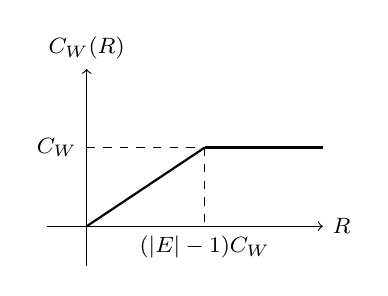
\begin{tikzpicture}
\tikzstyle{every node}=[font= \fontsize{8pt}{10pt}\selectfont]
    \draw [thin,  ->] (0,-0.5) -- (0,2)      % draw y-axis line
        node [above, black] {$\wskc(R)$};              % add label for y-axis
    
    \draw [thin,  ->] (-0.5,0) -- (3,0)      % draw x-axis line
        node [right, black] {$R$};              % add label for x-axis
    
    \draw [draw=black, thick] (0,0) -- (1.5,1);% draw the graph
    \draw [draw=black, thick] (1.5,1) -- (3,1);
    \draw [thin,  dashed] (0,1) -- (1.5,1);
    \draw [thin,  dashed] (1.5,1) -- (1.5,0);
    
    \node [left] at (0,1) {$\wskc$};                % label y-intercept
    \node [below] at (1.5,0) {$(|E|-1)\wskc$};               % label x-intercept
\end{tikzpicture}
\caption{$\wskc(R)$ curve denoting the wiretap secret key capacity at a given rate $R$ }
\label{fig:rateregion}
 \end{figure}
\begin{theorem}\label{thm:rate:irreducible}
Given an irreducible tree-PIN source $\RZ_V$ with a linear wiretapper $\RZ_w$, we have 
\begin{align*}
\wskc(R) = \min \left\{\frac{R}{|E|-1}, \wskc\right\} 
\end{align*}
where $R$ is the total discussion rate and $\wskc =\min_{e \in E}H(Y_e)$, which is the unconstrained wiretap secret key capacity.
\end{theorem}
\begin{proof}
Since the wiretapper side information can only reduce the secret key rate, $\wskc(R) \leq \skc(R)$. It follows from \cite[Theorem~4.2]{chan19} that $\skc(R) =  \min \left\{\frac{R}{|E|-1}, \skc\right\}$. Therefore, we have $\wskc(R) \leq \min \left\{\frac{R}{|E|-1}, \wskc\right\}$ because $\skc =\wskc$ for an irreducible tree-PIN source with a linear wiretapper, which was shown in Theorem~\ref{thm:cwsk:irred}.

For the achievability part, it is enough to show that the point $((|E|-1)\wskc,\wskc)$ is achievable because the rest of the curve follows from the time sharing argument between $((|E|-1)\wskc,\wskc)$ and $(0,0)$ ---  see Fig.~\ref{fig:rateregion}.

Let $s:=\wskc=\min_{e \in E}H(Y_e)=\min_{e \in E}n_e$, which is an integer. We will construct our achievable scheme on a sub-source  $\RZ'_V$ of the tree-PIN source $\RZ_V$ by ignoring some edge random variables. More precisely, $\RZ'_V$ is defined on the same tree $T$ with $\RY'_e := \left( \RX_{e,1}, \ldots, \RX_{e,s} \right)$ for each edge $e \in E$, and $\RZ'_i = \left( \RY'_e : i \in \xi (e) \right)$ for $i \in V$. Note that all the edge random vectors $\RY'_e$ have $s$ components. On the other hand, the  wiretapper side information $\RZ_{\opw}$ is the same as that of the original source. 

Let $\RX' :=(\RX_{e,k}: e\in E, 1 \leq k \leq s)$ and  $\RX'' :=(\RX_{e,k}: e\in E, s < k \leq n_e)$, which is a partition of the underlying components $\RX$ of the original source. This gives rise to a partition of the observations of the wiretapper into two parts: the first part contains observations involving only linear combinations of $\RX'$, and the second part contains linear observations with at least one component from $\RX''$. This means that $\RZ_{\opw}$, after applying some suitable invertible linear transformation, can be written as 
$$\RZ_{\opw} = \bM \RX' & \RX''\eM \bM \MA & \MB \\ \M{0} & \MC \eM ,$$ for some matrices $\MA$, $\MB$, and a full column-rank matrix $\MC$. With $\RZ'_{\opw}=\RX'\MA$ and $\RZ''_{\opw}=\RX'\MB + \RX''\MC$, $\RZ_{\opw} = \bM \RZ'_{\opw} & \RZ''_{\opw} \eM$.

For a large $n$,  users execute a linear secure omniscience communication scheme $\RF^{(n)}$ on the sub-source $\RZ'^n_V$ with respect to the wiretapper side information $\RZ^n_{\opw}$. Moreover, $\RF^{(n)}$ has the following properties: it achieves perfect omniscience at rate 
$$\frac{1}{n}H(\RF^{(n)})=H(\RZ'_V)-s=H(\RX')-s,$$ which is the minimum rate of omniscience $\rco(\RZ'_V)$, and it perfectly aligns with $\RZ'^n_{\opw}$, i.e., $H(\RZ'^n_{\opw}|\RF^{(n)})=0$. The existence of such a communication scheme is guaranteed from the proof of Theorem~\ref{thm:cwsk:irred}. After every user recovers the source $\RZ'^n_V$ using $\RF^{(n)}$, they agree on the key $\RK^{(n)}:=\RY'^n_{e_0}$ where $e_0 \in E$ is an edge incident on a leaf node. It is clear that $\RK^{(n)}$ satisfies the key recoverability condition because it is a function of the recovered source $\RZ'^n_V$. It remains to show that $\RK^{(n)}$ satisfies the secrecy condition.

Since $\RK^{(n)},\RZ'^n_{\opw}$ and $\RF^{(n)}$ are linear functions of $\RX'$, we have  $(\RK^{(n)}, \RF^{(n)}, \RZ'^n_{\opw}) - \RX'^n-\RZ''^n_{\opw}$. Note that $\RZ''^n_{\opw}$ is independent of $\RX'$ because $\MC$ is a full column-rank matrix. As a consequence, $\RZ''^n_{\opw}$ is independent of $(\RK^{(n)}, \RF^{(n)}, \RZ'^n_{\opw})$.  Furthermore, $\RY'^n_{e_0}$ is independent of $\RF^{(n)}$. This can be obtained by combining the perfect omniscience condition, which implies that $H(\RZ'^n_V|\RY'^n_{e_0},\RF^{(n)})=0$ for the leaf node, and the condition on the rate of the communication which is  $H(\RF^{(n)})=H(\RZ'^n_V)-ns=H(\RZ'^n_V)-H(\RY'^n_{e_0})$. Therefore, we have $H(\RY'^n_{e_0}|\RF^{(n)})= H(\RY'^n_{e_0},\RF^{(n)})-H(\RF^{(n)})=H(\RZ'^n_V,\RY'^n_{e_0},\RF^{(n)})-H(\RF^{(n)})=H(\RZ'^n_V)-H(\RF^{(n)})=H(\RY'^n_{e_0})$. The third equality is because $\RY'^n_{e_0}$ and $\RF^{(n)}$ are linear functions of $\RZ'^n_V$. Finally,
\begin{align*}
    H(\RK^{(n)}| \RF^{(n)}, \RZ^n_{\opw}) &=  H(\RK^{(n)}| \RF^{(n)}, \RZ'^n_{\opw},\RZ''^n_{\opw})\\
    &\utag{a}{=}  H(\RK^{(n)}| \RF^{(n)}, \RZ'^n_{\opw})\\
    &\utag{b}{=} H(\RK^{(n)}| \RF^{(n)})\\
    &= H(\RY'^n_{e_0}| \RF^{(n)})\\
    &\utag{c}{=}H(\RY'^n_{e_0})\\
    &= H(\RK^{(n)})
\end{align*}
where (a) follow from the independence of $\RZ''^n_{\opw}$ and $(\RK^{(n)}, \RF^{(n)}, \RZ'^n_{\opw})$, (b) is due that the fact that $\RF^{(n)}$ aligns perfectly with $\RZ'^n_{\opw}$, i.e., $H(\RZ'^n_{\opw}|\RF^{(n)})=0$ and (c) is because $\RY'^n_{e_0}$ is independent of $\RF^{(n)}$.

Thus we have shown that a secret key of rate $\frac{1}{n}H(\RK^{(n)})=\frac{1}{n}H(\RY'^n_{e_0})=s$ is achievable with a communication of rate $\frac{1}{n}H(\RF^{(n)})=H(\RZ'_V)-s= (|E|-1)s$. So the pair $((|E|-1)\wskc,\wskc)= ((|E|-1)s,s)$  is achievable, which is as desired.
\end{proof}

To extend this result to the general tree-PIN case, we will prove the following lemma, which allows us to carry out a reduction to an irreducible source without changing $\wskc(R)$. This lemma along with the above theorem on irreducible sources proves Theorem~\ref{thm:rateconstrained_treepin}. 

\begin{lemma}\label{lem:irred:rate} 
 If a tree-PIN source with a linear wiretapper $(\RZ_V,\RZ_{\opw})$ is not irreducible then there exists an irreducible source $(\tRZ_V, \tRZ_{\opw})$ such that 
 \begin{align*}
\wskc(\RZ_V\| \RZ_{\opw})(R) = \wskc(\tRZ_V\|\tRZ_{\opw})(R),\\ 
H(\RY_e|\op{mcf}(\RY_e\wedge\RZ_{\opw})) = H(\tRY_e)
\end{align*}
for all $e \in E$ and all discussion rates $R \geq 0$.
\end{lemma}
\begin{proof}
Since $(\RZ_V, \RZ_{\opw})$ is not irreducible, there exists an edge $e \in E$ such that $\RG_e := \op{mcf}(\RY_e\wedge \RZ_{\opw})$ is a non-constant function. Similar to the proof of Lemma~\ref{lem:irred:rate}, we linearly transform $\RY_e$ and $\RZ_{\opw}$ to  $(\RG_e, \tRY_e)$ and $(\RG_e, \tRZ_{\opw} )$, respectively where $ H(\tRY_e)=H(\RY_e|\op{mcf}(\RY_e\wedge\RZ_{\opw}))$. Let us consider a  new tree-PIN  source $\tRZ_V$, which is the same as $\RZ_V$ except that  $\tRY_e$ and $\tilde{n}_e$ are associated to the edge $e$, and the wiretapper side information is  $\tRZ_{\opw}$. Note that $(\tRZ_V, \tRZ_{\opw})$ is also a tree-PIN source with a linear wiretapper, and $\RG_e$ is independent of $(\tRZ_V, \tRZ_{\opw})$.

Since any valid scheme on reduced model $(\tRZ_V, \tRZ_{\opw})$ can be used as a valid scheme on original model $(\RZ_V, \RZ_{\opw})$, we have 
$$\wskc(\RZ_V\| \RZ_{\opw})(R) \geq \wskc(\tRZ_V\|\tRZ_{\opw})(R).$$

To prove the reverse inequality, $\wskc(R):=\wskc(\RZ_V\| \RZ_{\opw})(R) \leq \wskc(\tRZ_V\|\tRZ_{\opw})(R)$, consider capacity-optimal schemes. Fix $\delta>0$, and let $(\RF^{(n)},\RK^{(n)})$ be a WSKA scheme whose key rate and communication rate satisfy
\begin{gather}
    \wskc(R)-\delta < \liminf \frac{1}{n}\log|\mc{K}^{(n)}| < \wskc(R), \label{eq:rate_k}\\
    \limsup \frac{1}{n}\log|\mc{F}^{(n)}| < R. \nonumber
\end{gather}
Let $L:=\liminf \frac{1}{n}\log|\mc{K}^{(n)}|$. Fix an $\epsilon>0$ small enough that $(L-7\epsilon, L+7\epsilon) \subseteq (\wskc(R)-\delta, \wskc(R))$.
We restrict to a subsequence of $\left(\frac{1}{n}\log|\mc{K}^{(n)}|\right)_{n\geq 1}$ whose limit is $L$. And, with an abuse of notation, we still index this sequence\footnote{Designing a protocol on a subsequence can easily be extended to all the integers without sacrificing the asymptotic performance of the protocol.} with $n$. Therefore, for all $n$ large enough,  $L-\epsilon <\frac{1}{n}\log|\mc{K}^{(n)}| < L+\epsilon$. Again, along this subsequence, we have $\limsup \frac{1}{n}\log|\mc{F}^{(n)}| < R$ because of the properties of subsequential limits. Moreover, we have  $0 \leq \log|\mc{K}^{(n)}|-H(\RK^{(n)}|\RZ^n_{\opw},\RF^{(n)})=\left[\log|\mc{K}^{(n)}|-H(\RK^{(n)})\right] +I(\RK^{(n)} \wedge \RZ^n_{\opw},\RF^{(n)})< \epsilon$ and $\Pr\left[ \exists j\in V \text{ s.t. }  \RK_j^{(n)}\neq \RK^{(n)}\right]< \epsilon$ for all $n$ large enough.

Note that the above secrecy  condition implies that $0\leq\left[\log|\mc{K}^{(n)}|-H(\RK^{(n)})\right] < \epsilon$ and  $I(\RK^{(n)}\wedge\tRZ^n_{\opw},\RG^n_e,\RF^{(n)})=I(\RK^{(n)}\wedge\RZ^n_{\opw},\RF^{(n)})<  \epsilon$. The latter condition implies that $I(\RK^{(n)}\wedge\tRZ^n_{\opw},\RF^{(n)}|\RG^n_e)<  \epsilon$ and $I(\RK^{(n)}\wedge \RG^n_e)<  \epsilon$. From all the above conditions, we have
\begin{gather}
L-\epsilon <\frac{1}{n}\log|\mc{K}^{(n)}| < L+\epsilon,\label{eq:rate1}\\
    0\leq\left[\log|\mc{K}^{(n)}|-H(\RK^{(n)})\right] < \epsilon,\label{eq:rate2}\\
    I(\RK^{(n)}\wedge\tRZ^n_{\opw},\RF^{(n)}|\RG^n_e)<  \epsilon,\label{eq:rate3}\\ I(\RK^{(n)}\wedge \RG^n_e)<  \epsilon.\label{eq:rate4}
\end{gather}
Let $\mc{K}^{(n)}_g$ be the range of $\RK^{(n)}$ when $\RG_e^n=g$, and similarly, $\mc{F}^{(n)}_g$ denote the range of $\RF^{(n)}$ when $\RG_e^n=g$. Note that since $\mc{K}^{(n)}_g \subseteq \mc{K}^{(n)}$ and $\mc{F}^{(n)}_g \subseteq \mc{F}^{(n)}$ for any $g$, we have $\log|\mc{K}^{(n)}_g|\leq \log|\mc{K}^{(n)}|$ and $\log|\mc{F}^{(n)}_g|\leq \log|\mc{F}^{(n)}|$, hence
\begin{gather}
    \sum_{g}\Pr(\RG_e^n=g)\log|\mc{K}^{(n)}_g|\leq  \log|\mc{K}^{(n)}|.\label{eq:rate5}
\end{gather}
We will show that there exists a realization $g^{*}$ of $\RG_e^n$ for which all the desired conditions are met.

From \eqref{eq:rate2}, \eqref{eq:rate4} and \eqref{eq:rate5}, we obtain
\begin{gather*}
    H(\RK^{(n)}|\RG^n_e)\leq \sum_{g}\Pr(\RG_e^n=g) \log|\mc{K}^{(n)}_g|\leq \log|\mc{K}^{(n)}| < H(\RK^{(n)}|\RG^n_e)+2\epsilon.
\end{gather*}
We can conclude from the above chain of inequalities that 
\begin{gather*}
    0\leq \sum_{g}\Pr(\RG_e^n=g)\left[\frac{1}{n} \log|\mc{K}^{(n)}|-\frac{1}{n} \log|\mc{K}^{(n)}_g|\right]< 2\epsilon,\\
    0\leq \sum_{g}\Pr(\RG_e^n=g)\left[ \log|\mc{K}_g^{(n)}|-H(\RK^{(n)}|\RG^n_e=g)\right]< 2\epsilon.
\end{gather*}
These inequalities together with \eqref{eq:rate3} give
\begin{align*}
    0\leq &\sum_{g}\Pr(\RG_e^n=g)\left\lbrace\left[\frac{1}{n} \log|\mc{K}^{(n)}|-\frac{1}{n} \log|\mc{K}^{(n)}_g|\right]+\left[ \log|\mc{K}_g^{(n)}|-H(\RK^{(n)}|\RG^n_e=g)\right]\right. \\ &\left.+\, I(\RK^{(n)}\wedge\tRZ^n_{\opw},\RF^{(n)}|\RG^n_e=g)+\Pr\left( \exists j\in V \text{ s.t. } \RK_j^{(n)}\neq \RK^{(n)}\Bigm\vert \RG^n_e=g\right)\right\rbrace < 5\epsilon.
\end{align*}
Note that the averaged quantity (the term in the curly bracket) is non-negative; hence there exists a realization of $\RG_e^{(n)}=g^*$ such that 
\begin{align*}
    0\leq &\left[\frac{1}{n} \log|\mc{K}^{(n)}|-\frac{1}{n} \log|\mc{K}^{(n)}_{g^*}|\right]+\left[ \log|\mc{K}_{g^*}^{(n)}|-H(\RK^{(n)}|\RG^n_e={g^*})\right]\\ &+\,I(\RK^{(n)}\wedge\tRZ^n_{\opw},\RF^{(n)}|\RG^n_e={g^*})+\Pr\left( \exists j\in V \text{ s.t. } \RK_j^{(n)}\neq \RK^{(n)}\Bigm\vert \RG^n_e=g\right) < 5\epsilon.
\end{align*}
Since all the summands are non-negative, we have 
\begin{subequations}
\label{eq:rate6}
\begin{gather}
    0\leq \left[\frac{1}{n} \log|\mc{K}^{(n)}|-\frac{1}{n} \log|\mc{K}^{(n)}_{g^*}|\right]< 5\epsilon,\label{eq:rate7}\\
    0\leq \left[ \log|\mc{K}_{g^*}^{(n)}|-H(\RK^{(n)}|\RG^n_e={g^*})\right]< 5\epsilon,\label{eq:rate8}\\ 
    0\leq I(\RK^{(n)}\wedge\tRZ^n_{\opw},\RF^{(n)}|\RG^n_e={g^*}) < 5\epsilon,\label{eq:rate9}\\
    0\leq \Pr\left( \exists j\in V \text{ s.t. } \RK_j^{(n)}\neq \RK^{(n)}\Bigm\vert \RG^n_e=g^*\right) < 5\epsilon\label{eq:rate10}.
\end{gather}
\end{subequations}
Let $\RK^{(n)}_{j, g^*}$ (resp. $\RF^{(n)}_{g^*}$) be the function  $\RK^{(n)}_j$ (resp. $\RF^{(n)}$) restricted to $\RG^n_e={g^*}$. So $\RK^{(n)}_{j, g^*}$ and $\RF^{(n)}_{g^*}$ are  functions solely of $\tRZ_V^n$ and possible private randomness. For the source $(\tRZ_V, \tRZ_{\opw})$, users run the scheme $(\RF^{(n)}_{g^*},\RK^{(n)}_{1, g^*}, \ldots, \RK^{(n)}_{m, g^*})$ to generate a secret key using the source $\tRZ_V^n$ and the private randomness. It is enough to argue that this a valid WSKA scheme. To see this, let $P_{\RK^{(n)},\tRZ_V^n, \tRZ_{\opw}^n,\RS_V,\RG^n_e}$ be the joint distribution of $\RK^{(n)}$ and the source random variables, where $\RS_V$ is the local randomness generated by the users. Consider a random variable $\RK^{(n)}_{g^*}$ whose joint distribution with the other random variables is $P_{\RK^{(n)}_{g^*},\tRZ_V^n, \tRZ_{\opw}^n,\RS_V}=P_{\RK^{(n)}|\tRZ_V^n, \tRZ_{\opw}^n,\RS_V,\RG^n_e=g^*}\cdot P_{\tRZ_V^n, \tRZ_{\opw}^n,\RS_V}$. Since $\RG^n_e$ is independent of $(\tRZ_V^n, \tRZ_{\opw}^n,\RS_V)$, we have $H(\RK^{(n)}_{g^*})=H(\RK^{(n)}|\RG^n_e={g^*})$, $I(\RK^{(n)}_{g^*}\wedge\tRZ^n_{\opw},\RF^{(n)})=I(\RK^{(n)}\wedge\tRZ^n_{\opw},\RF^{(n)}|\RG^n_e={g^*})$ and $\Pr\left( \exists j\in V \text{ s.t. } \RK_{j, g^*}^{(n)}\neq \RK_{g^*}^{(n)}\right)=\Pr\left( \exists j\in V \text{ s.t. } \RK_j^{(n)}\neq \RK^{(n)}\Bigm\vert \RG^n_e=g^*\right)$. As $\epsilon>0$ is arbitrary, the conditions \eqref{eq:rate10}, \eqref{eq:rate9}, and \eqref{eq:rate8} imply that recoverability and secrecy conditions are met, proving that this is a valid WSKA scheme. Moreover, the rate of this code satisfies
$\liminf \frac{1}{n} \log|\mc{K}^{(n)}_{g^*}|> \liminf \frac{1}{n} \log|\mc{K}^{(n)}|-6 \epsilon > L-7\epsilon$. From the assumption that $(L-7\epsilon, L+7\epsilon) \subseteq (\wskc(R)-\delta, \wskc(R))$, we have $\liminf \frac{1}{n} \log|\mc{K}^{(n)}_{g^*}|>\wskc(R)-\delta$. Furthermore, the rate of the communication $\RF^{(n)}_{g^*}$ satisfies $\limsup\frac{1}{n}\log|\mc{F}^{(n)}_{g^*}|\leq \limsup\frac{1}{n}\log|\mc{F}^{(n)}| < R$.
Thus,
\begin{align*}
    \wskc(\tRZ_V\|\tRZ_{\opw})(R)>\wskc(\RZ_V\| \RZ_{\opw})(R)-\delta.
\end{align*}
As $\delta$ is arbitrary, we have $\wskc(\tRZ_V\|\tRZ_{\opw})(R)
\geq \wskc(\RZ_V\| \RZ_{\opw})(R).$
This shows that  $\wskc(\RZ_V\| \RZ_{\opw})(R)= \wskc(\tRZ_V\|\tRZ_{\opw})(R)$. Therefore, we can repeat this process until the source becomes irreducible without affecting $\wskc(\RZ_V\| \RZ_{\opw})(R)$.
\end{proof}

The result of Theorem~\ref{thm:rateconstrained_treepin} follows by putting the above lemma and theorem together.





% Similar to the unconstrained case, we first prove the result for irreducible sources and then argue that the rate region of a general source is the same as that of an irreducible source that is obtained through reduction.
% \begin{figure}[h]
% \centering
% 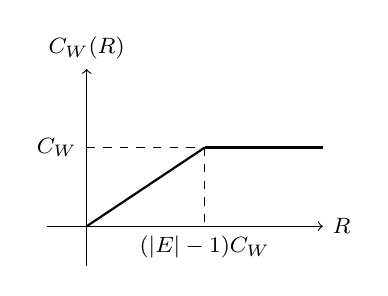
\begin{tikzpicture}
\tikzstyle{every node}=[font= \fontsize{8pt}{10pt}\selectfont]
    \draw [thin,  ->] (0,-0.5) -- (0,2)      % draw y-axis line
        node [above, black] {$\wskc(R)$};              % add label for y-axis
    
    \draw [thin,  ->] (-0.5,0) -- (3,0)      % draw x-axis line
        node [right, black] {$R$};              % add label for x-axis
    
    \draw [draw=black, thick] (0,0) -- (1.5,1);% draw the graph
    \draw [draw=black, thick] (1.5,1) -- (3,1);
    \draw [thin,  dashed] (0,1) -- (1.5,1);
    \draw [thin,  dashed] (1.5,1) -- (1.5,0);
    
    \node [left] at (0,1) {$\wskc$};                % label y-intercept
    \node [below] at (1.5,0) {$(|E|-1)\wskc$};               % label x-intercept
\end{tikzpicture}
% \caption{$\wskc(R)$ curve denoting the wiretap secret key capacity at a given rate $R$ }
% \label{fig:rateregion}
%  \end{figure}
% \begin{theorem}
% Given an irreducible tree-PIN source $\RZ_V$ with a linear wiretapper $\RZ_w$, we have 
% \begin{align*}
% \wskc(R) = \min \left\{\frac{R}{|E|-1}, \wskc\right\} 
% \end{align*}
% where $R$ is the total discussion rate and $\wskc =\min_{e \in E}H(Y_e)$, which is the unconstrained wiretap secret key capacity.
% \end{theorem}
% \begin{proof}
% Since the wiretapper side information can only reduce the secret key rate, $\wskc(R) \leq \skc(R)$. It follows from \cite[Theorem~4.2]{chan19} that $\skc(R) =  \min \left\{\frac{R}{|E|-1}, \skc\right\}$. Therefore, we have $\wskc(R) \leq \min \left\{\frac{R}{|E|-1}, \wskc\right\}$ because $\skc =\wskc$ for an irreducible tree-PIN source with linear wiretapper, which was shown in Theorem~\ref{thm:cwsk:irred}.

% For the achievability part, it is enough to show that the point $((|E|-1)\wskc,\wskc)$ is achievable because the rest of the curve follows from the time sharing argument between $((|E|-1)\wskc,\wskc)$ and $(0,0)$ ---  see Fig.~\ref{fig:rateregion}.

% Let $s:=\wskc=\min_{e \in E}H(Y_e)=\min_{e \in E}n_e$, which is an integer. We will construct our achievable scheme on a sub-source  $\RZ'_V$ of the tree-PIN source $\RZ_V$ by ignoring some edge random variables. More precisely, $\RZ'_V$ is defined on the same tree $T$ with $\RY'_e := \left( \RX_{e,1}, \ldots, \RX_{e,s} \right)$ for each edge $e \in E$, and $\RZ'_i = \left( \RY'_e : i \in \xi (e) \right)$ for $i \in V$. Note that all the edge random vectors $\RY'_e$ have $s$ components. On the other hand, the  wiretapper side information $\RZ_{\opw}$ is the same as that of the original source. 

% Let $\RX' :=(\RX_{e,k}: e\in E, 1 \leq k \leq s)$ and  $\RX'' :=(\RX_{e,k}: e\in E, s < k \leq n_e)$, which is a partition of the underlying components $\RX$ of the original source. This gives rise to a partition of the observations of the wiretapper into two parts: the first part contains observations involving only linear combinations of $\RX'$, and the second part contains linear observations with at least one component from $\RX''$. This means that $\RZ_{\opw}$, after applying some suitable invertible linear transformation, can be written as 
% $$\RZ_{\opw} = \bM \RX' & \RX''\eM \bM \MA & \MB \\ \M0 & \MC \eM ,$$ for some matrices $\MA$, $\MB$, and a full column-rank matrix $\MC$. With $\RZ'_{\opw}=\RX'\MA$ and $\RZ''_{\opw}=\RX'\MB + \RX''\MC$, $\RZ_{\opw} = \bM \RZ'_{\opw} & \RZ''_{\opw} \eM$.

% For a large $n$,  users execute a linear secure omniscience communication scheme $\RF^{(n)}$ on the sub-source $\RZ'^n_V$ with respect to the wiretapper side information $\RZ^n_{\opw}$. Moreover, $\RF^{(n)}$ has the following properties: it achieves perfect omniscience at rate 
% $$\frac{1}{n}H(\RF^{(n)})=H(\RZ'_V)-s=H(\RX')-s,$$ which is the minimum rate of omniscience $\rco(\RZ'_V)$, and it perfectly aligns with $\RZ'^n_{\opw}$, i.e., $H(\RZ'^n_{\opw}|\RF^{(n)})=0$. The existence of such a communication scheme is guaranteed from the proof of Theorem~\ref{thm:cwsk:irred}. After every user recovers the source $\RZ'^n_V$ using $\RF^{(n)}$, they agree on the key $\RK^{(n)}:=\RY'^n_{e_0}$ where $e_0 \in E$ is an edge incident on a leaf node. It is clear that $\RK^{(n)}$ satisfies the key recoverability condition because it is a function of the recovered source $\RZ'^n_V$. It remains to show that $\RK^{(n)}$ satisfies the secrecy condition.

% Since $\RK^{(n)},\RZ'^n_{\opw}$ and $\RF^{(n)}$ are linear functions of $\RX'$, we have  $(\RK^{(n)}, \RF^{(n)}, \RZ'^n_{\opw}) - \RX'^n-\RZ''^n_{\opw}$. Note that $\RZ''^n_{\opw}$ is independent of $\RX'$ because $\MC$ is a full column-rank matrix. As a consequence, $\RZ''^n_{\opw}$ is independent of $(\RK^{(n)}, \RF^{(n)}, \RZ'^n_{\opw})$.  Furthermore, $\RY'^n_{e_0}$ is independent of $\RF^{(n)}$. This can be obtained by combining the perfect omniscience condition, which implies that $H(\RZ'^n_V|\RY'^n_{e_0},\RF^{(n)})=0$ for the leaf node, and the condition on the rate of the communication which is  $H(\RF^{(n)})=H(\RZ'^n_V)-ns=H(\RZ'^n_V)-H(\RY'^n_{e_0})$. Therefore, we have $H(\RY'^n_{e_0}|\RF^{(n)})= H(\RY'^n_{e_0},\RF^{(n)})-H(\RF^{(n)})=H(\RZ'^n_V,\RY'^n_{e_0},\RF^{(n)})-H(\RF^{(n)})=H(\RZ'^n_V)-H(\RF^{(n)})=H(\RY'^n_{e_0})$. The third equality is because $\RY'^n_{e_0}$ and $\RF^{(n)}$ are linear functions of $\RZ'^n_V$. Finally,
% \begin{align*}
%     H(\RK^{(n)}| \RF^{(n)}, \RZ^n_{\opw}) &=  H(\RK^{(n)}| \RF^{(n)}, \RZ'^n_{\opw},\RZ''^n_{\opw})\\
%     &\utag{a}{=}  H(\RK^{(n)}| \RF^{(n)}, \RZ'^n_{\opw})\\
%     &\utag{b}{=} H(\RK^{(n)}| \RF^{(n)})\\
%     &= H(\RY'^n_{e_0}| \RF^{(n)})\\
%     &\utag{c}{=}H(\RY'^n_{e_0})\\
%     &= H(\RK^{(n)})
% \end{align*}
% where (a) follow from the independence of $\RZ''^n_{\opw}$ and $(\RK^{(n)}, \RF^{(n)}, \RZ'^n_{\opw})$, (b) is due that the fact that $\RF^{(n)}$ aligns perfectly with $\RZ'^n_{\opw}$, i.e., $H(\RZ'^n_{\opw}|\RF^{(n)})=0$ and (c) is because $\RY'^n_{e_0}$ is independent of $\RF^{(n)}$.

% Thus we have shown that a secret key of rate $\frac{1}{n}H(\RK^{(n)})=\frac{1}{n}H(\RY'^n_{e_0})=s$ is achievable with a communication of rate $\frac{1}{n}H(\RF^{(n)})=H(\RZ'_V)-s= (|E|-1)s$. So the pair $((|E|-1)\wskc,\wskc)= ((|E|-1)s,s)$  is achievable, which is as desired.
% \end{proof}

% To extend this result to the general tree-PIN case, we will prove the following lemma, which allows us to carry out a reduction to an irreducible source without changing $\wskc(R)$. This lemma along with the above theorem on irreducible sources proves Theorem~\ref{thm:rateconstrained_treepin}. 

% \begin{lemma}\label{lem:irred:rate} 
%  If a tree-PIN source with linear wiretapper $(\RZ_V,\RZ_{\opw})$ is not irreducible then there exists an irreducible source $(\tRZ_V, \tRZ_{\opw})$ such that 
%  \begin{align*}
% &\wskc(\RZ_V\| \RZ_{\opw})(R) = \wskc(\tRZ_V\|\tRZ_{\opw})(R),\\ 
% &H(\RY_e|\op{mcf}(\RY_e,\RZ_{\opw})) = H(\tRY_e),
% \end{align*}
% for all $e \in E$.
% \end{lemma}
% \begin{proof}
% Since $(\RZ_V, \RZ_{\opw})$ is not irreducible, there exists an edge $e \in E$ such that $\RG_e := \op{mcf}(\RY_e, \RZ_{\opw})$ is a non-constant function. Similar to the proof of Lemma~\ref{lem:irred:rate}, we linearly transform $\RY_e$ and $\RZ_{\opw}$ to  $(\RG_e, \tRY_e)$ and $(\RG_e, \tRZ_{\opw} )$, respectively where $ H(\tRY_e)=H(\RY_e|\op{mcf}(\RY_e,\RZ_{\opw}))$. Let us consider a  new tree-PIN  source $\tRZ_V$, which is the same as $\RZ_V$ except that  $\tRY_e$ and $\tilde{n}_e$ are associated to the edge $e$, and the wiretapper side information is  $\tRZ_{\opw}$. Note that $(\tRZ_V, \tRZ_{\opw})$ is also a tree-PIN source with linear wiretapper, and $\RG_e$ is independent of $(\tRZ_V, \tRZ_{\opw})$.

% Since any valid scheme on reduced model $(\tRZ_V, \tRZ_{\opw})$ can be used as a valid scheme on original model $(\RZ_V, \RZ_{\opw})$, we have 
% $$\wskc(\RZ_V\| \RZ_{\opw})(R) \geq \wskc(\tRZ_V\|\tRZ_{\opw})(R).$$

% To prove the reverse inequality, $\wskc(\RZ_V\| \RZ_{\opw})(R) \leq \wskc(\tRZ_V\|\tRZ_{\opw})(R)$, let $(\RF^{(n)},\RK^{(n)})$ be an SKA scheme achieving $\wskc(\RZ_V\| \RZ_{\opw})(R)=:\wskc(R)$. It means that for $\epsilon_n \to 0$ 
% \begin{align*}
%     & \left|\frac{1}{n}H(\RF^{(n)})-R \right|< \epsilon_n ,\quad \left|\frac{1}{n}H(\RK^{(n)})-\wskc(R)\right|< \epsilon_n, \notag\\
%     & I(\RK^{(n)}\wedge\RZ^n_{\opw},\RF^{(n)})< \epsilon_n, \text{ and }
%     \Pr\left[ \exists j\in V \text{ s.t. } \RK_j^{(n)}\neq \RK_1^{(n)}\right]< \epsilon_n. \notag
% \end{align*}
% Note that the condition $I(\RK^{(n)}\wedge\tRZ^n_{\opw},\RG^n_e,\RF^{(n)})=I(\RK^{(n)}\wedge\RZ^n_{\opw},\RF^{(n)})< \epsilon_n$ implies that $I(\RK^{(n)}\wedge\tRZ^n_{\opw},\RF^{(n)}|\RG^n_e)< \epsilon_n$ and $I(\RK^{(n)}\wedge \RG^n_e)< \epsilon_n$, which in turn imply that $H(\RK^{(n)}) -H(\RK^{(n)}|\RG^n_e)< \epsilon_n$ and $\left|\frac{1}{n}H(\RK^{(n)}|\RG^n_e)-\wskc(R)\right|<2\epsilon_n$. The last inequality follows  from the triangle inequality. Since $\frac{1}{n}H(\RF^{(n)}|\RG^n_e)\leq \frac{1}{n}H(\RF^{(n)})$ and  $\frac{1}{n}H(\RF^{(n)}) \to R$, we have  $\limsup \frac{1}{n}H(\RF^{(n)}|\RG^n_e)\leq R$. We just  restrict to the subsequence  whose limit achieves limsup and with an abuse of notation we still index this sequence with $n$. Let $\lim \frac{1}{n}H(\RF^{(n)}|\RG^n_e):=R-\gamma$ for some $\gamma\geq 0$.

% Now we will find  a best realization of $\RG_e^n$ for which the SKA scheme $(\RF^{(n)},\RK^{(n)})$ has desired properties. From all the above conditions, we have 
% \begin{align*}
%     &\left|\frac{1}{n}H(\RF^{(n)}|\RG^n_e)-(R-\gamma) \right| + \left|\frac{1}{n}H(\RK^{(n)}|\RG^n_e)-\wskc(R)\right|+I(\RK^{(n)}\wedge\tRZ^n_{\opw},\RF^{(n)}|\RG^n_e)\\&\mkern 400mu+\Pr\left[ \exists j\in V \text{ s.t. } \RK_j^{(n)}\neq \RK_1^{(n)}\right]< 5\epsilon_n.
% \end{align*}
% We can rewrite it as 
% \begin{align*}
%     &\sum \Pr(\RG^n_e=g^n_e)\left\{\left|\frac{1}{n}H(\RF^{(n)}|\RG^n_e=g^n_e)-(R-\gamma) \right| + \left|\frac{1}{n}H(\RK^{(n)}|\RG^n_e=g^n_e)-\wskc(R)\right|\right.\\&\mkern 100mu\left.+I(\RK^{(n)}\wedge\tRZ^n_{\opw},\RF^{(n)}|\RG^n_e=g^n_e)+\Pr\left[ \exists j\in V \text{ s.t. } \RK_j^{(n)}\neq \RK_1^{(n)}|\RG^n_e=g^n_e\right]\right\}< 5\epsilon_n. 
% \end{align*}
% Since the average is less than $5\epsilon_n$, there exists a realization $\RG^n_e=g^n_e$ such that 
% \begin{align}\label{eq:rate:reduction}
%     &\left|\frac{1}{n}H(\RF^{(n)}|\RG^n_e=g^n_e)-(R-\gamma) \right|\notag +\left|\frac{1}{n}H(\RK^{(n)}|\RG^n_e=g^n_e)-\wskc(R)\right|\notag +I(\RK^{(n)}\wedge\tRZ^n_{\opw},\RF^{(n)}|\RG^n_e=g^n_e)\notag \\&\mkern 400mu+\Pr\left[ \exists j\in V \text{ s.t. } \RK_j^{(n)}\neq \RK_1^{(n)}|\RG^n_e=g^n_e\right]< 5\epsilon_n.
% \end{align}
% Therefore, each term in the summation is less than $5\epsilon_n$. Now we can use the scheme $(\RF^{(n)},\RK^{(n)})$  corresponding to a fixed $\RG^n_e=g^n_e$ on the reduced model $(\tRZ_V, \tRZ_{\opw})$. From \eqref{eq:rate:reduction}, we can say that it is a valid SKA scheme on $(\tRZ_V, \tRZ_{\opw})$  with a key rate of $\wskc(R)$ and a communication rate of  $(R-\gamma)$. Thus,
% \begin{align*}
%     \wskc(\RZ_V\| \RZ_{\opw})(R)= \wskc(R) \leq \wskc(\tRZ_V\|\tRZ_{\opw})(R-\gamma)\leq \wskc(\tRZ_V\|\tRZ_{\opw})(R),
% \end{align*}
% where the first inequality is due the fact that capacity is the maximum of all the achievable rates at a communication rate of $(R-\gamma)$, and the last inequality follows form the  monotonicity of the $\wskc(R)$ curve. This shows that  $\wskc(\RZ_V\| \RZ_{\opw})(R)= \wskc(\tRZ_V\|\tRZ_{\opw})(R)$. Therefore, we can repeat this process until the source becomes irreducible without affecting $\wskc(\RZ_V\| \RZ_{\opw})(R)$.
% \end{proof}

% The result of Theorem~\ref{thm:rateconstrained_treepin} follows by putting the above lemma and theorem together.



 

% \section{Proof of Theorem~\ref{thm:multivariate_positivity}} \label{app:multivariate_positivity}
% Some of the steps in the proof are analogous to the proof for the two-user case, \cite[Theorem~4]{amin2020}.  The new component of the theorem is the identification of a connection between the positivity of $\wskc$ and the non-maximality of $\rl$ of a transformed source.
Since most of the essential ideas of the two-user setting work even in the multiuser case, we only give proof sketches for these analogous steps. However, the new arguments are described in detail.


% we only provide new key arguments  and give proof sketches for the analogous arguments.

The statement 3) implies 4) is trivial. So it is enough to show that 1) implies 2), 2) implies 3), and 4) implies 1).

\textit{1) implies 2):} We prove this by following an approach that is similar to that of the two-user case. First, using the sets given in 1), we construct a new source $(\tRZ_V,\tRZ_{\opw})$ by applying some functions to the user random variables of the source $(\RZ^r_V,\RZ^r_{\opw})$. Then, we show that $\wskc(\tRZ_V||\tRZ_{\opw})>0$ which in turn implies that $\wskc(\RZ_V||\RZ_{\opw})>0$ because any SKA scheme on the source $(\tRZ_V,\tRZ_{\opw})$ is an SKA scheme on $(\RZ_V,\RZ_{\opw})$. To prove $\wskc(\tRZ_V||\tRZ_{\opw})>0$ using condition 1), we use the lower bound of Theorem~\ref{thm:RL:lb} and Lemma~\ref{lem:hatsource} for the new source.


Let $(\tRZ_1,\ldots,\tRZ_m,\tRZ_{\opw})$ be a function of $(\RZ^r_1,\ldots,\RZ^r_m,\RZ^r_{\opw})$ obtained by setting $\tRZ_i = 1$ if $\RZ_i^r \in \mc{A}_{i1}$, $\tRZ_i = 2$ if $\RZ_i^r \in \mc{A}_{i2}$ and  $\tRZ_i = 3$ if $\RZ_i^r \not\in \mc{A}_{i1}\cup \mc{A}_{i2}$ for $1\leq i\leq m$, and $\tRZ_{\opw} = \RZ_{\opw}^r$. Let $p_{j_1\ldots j_m} :=\Pr(\tRZ_1=j_1, \ldots, \tRZ_m=j_m)= \Pr(\RZ^r_1 \in \mcA_{1j_1}, \ldots, \tRZ_m\in \mcA_{mj_m})$ for all $(j_1, \ldots, j_m) \in \{1,2\}^m$. The condition in 1) is equivalent  to the condition 
\begin{align*}
       &D_{\frac{1}{2}} \left(P_{\tRZ_{\opw}}(.|\tRZ_1=1, \ldots, \tRZ_m=1)  
       %\right. \\& \mkern 100mu \left.
       ||P_{\tRZ_{\opw}}(.|\tRZ_1=2, \ldots, \tRZ_m=2) \right)
       < \log \left(\frac{p_{1,1,\ldots,1}p_{2,2,\ldots,2}}{\sum \limits_{\substack{(j_1,\ldots,j_m)\\ \not\in \{(1,\ldots,1),\\\mkern 30mu (2,\ldots,2)\}}}\dfrac{p_{j_1, \ldots, j_m}p_{3-j_1,\ldots, 3-j_m}}{2}}\right).
 \end{align*}
 
 
 We will show that the above condition implies 
  \begin{align} \label{eq:rco_nonmaximal}
     &H(\tRZ^n_V|\tRZ^n_{\opw},\tRZ^n_V\in \mc{A}_{1}\times\cdots\times\mc{A}_{m})
    %\notag \\& \mkern 100mu  
     > \rco(\tRZ^n_V|\tRZ^n_V\in \mc{A}_{1}\times\cdots\times\mc{A}_{m})
 \end{align}
 for some integer $n$, and a non-empty set $\mc{A}_{1}\times\cdots\times\mc{A}_{m}$, where $\mc{A}_{i} \subset \{1,2\}^n$ for all $i \in V$. Because of the following argument, inequality \eqref{eq:rco_nonmaximal} implies that $\wskc(\tRZ_V||\tRZ_{\opw})>0$ which further implies that $\wskc(\RZ_V||\RZ_{\opw})>0$. Suppose that there is an integer $n$, and a non-empty set $\mc{A}_{1}\times\cdots\times\mc{A}_{m}\subset \{1,2\}^n\times\cdots\times \{1,2\}^n$ such that \eqref{eq:rco_nonmaximal} holds. Let $(\widehat{\tRZ_V^n},\tRZ^n_{\opw})$ be the source as defined in \eqref{eq:hatsource} using the source $(\tRZ_V^n,\tRZ^n_{\opw})$ and the set $\mc{A}_{1}\times\cdots\times\mc{A}_{m}$.  Condition \eqref{eq:rco_nonmaximal} can be written as $H(\widehat{\tRZ_V^n}|\tRZ^n_{\opw})> \rco(\widehat{\tRZ_V^n})$. For the new source, it follows from \eqref{eq:rl_rco} that 
 \begin{align*}
     \rl(\widehat{\tRZ_V^n}||\tRZ^n_{\opw}) \leq \rco(\widehat{\tRZ_V^n}).
 \end{align*}
Therefore, we have  $H(\widehat{\tRZ_V^n}|\tRZ^n_{\opw})-\rl(\widehat{\tRZ_V^n}||\tRZ^n_{\opw}) \geq H(\widehat{\tRZ_V^n}|\tRZ^n_{\opw})- \rco(\widehat{\tRZ_V^n})>0$. By combining this with Lemma~\ref{lem:hatsource}, we get 
$H(\tRZ_V^n|\tRZ^n_{\opw})-\rl(\tRZ_V^n||\tRZ^n_{\opw}) \geq \Pr(\mcE) [H(\widehat{\tRZ_V^n}|\tRZ^n_{\opw})-\rl(\widehat{\tRZ_V^n}||\tRZ^n_{\opw})]>0$. So we conclude that $H(\tRZ_V|\tRZ_{\opw})-\rl(\RZ_V||\tRZ_{\opw})=\dfrac{1}{n}[H(\tRZ_V^n|\tRZ^n_{\opw})-\rl(\tRZ_V^n||\tRZ^n_{\opw})]>0$. Hence, it follows from the lower bound of Theorem~\ref{thm:RL:lb} that if $\rl(\tRZ_V||\tRZ_{\opw})< H(\tRZ_V|\tRZ_{\opw})$ then $\wskc(\tRZ_V||\tRZ_{\opw})>0$. Since the source $(\tRZ_V, \tRZ_{\opw})$ is obtained by processing (deterministically) each user observations of the source $(\RZ^r_V, \RZ^r_{\opw})$, any positive rate secret key on $(\tRZ_V, \tRZ_{\opw})$ is also a positive rate secret key on $(\RZ^r_V, \RZ^r_{\opw})$. Thus $\wskc(\tRZ_V||\tRZ_{\opw})>0$ implies that $\wskc(\RZ_V||\RZ_{\opw})= \frac{1}{r}\wskc(\RZ^r_V|| \RZ^r_{\opw})>0$.\\


Now we will show  that condition 1) implies \eqref{eq:rco_nonmaximal}.
Consider the following repetition coding with block swapping: for an even integer $n$, let
 \begin{align*}
  \mathbf{1}&:=\underbrace{1\ldots 1}_{n/2}\underbrace{ 2\ldots 2}_{n/2}\\
  \mathbf{2}&:=2\ldots 2 1\ldots 1
 \end{align*}
 and $\mc{A}_{i}:=\{\mathbf{1},\mathbf{2}\}$, for $1\leq i\leq m$. Let us define $\mc{A}_{V}:=\mc{A}_{1}\times\cdots\times\mc{A}_{m}$. It is enough to show that for large enough $n$, 
\begin{align}\label{eq:non_maximal_1}
     H(\tRZ^n_V|\tRZ^n_{\opw},\tRZ^n_V\in \mc{A}_{V}) > \rco(\tRZ^n_V|\tRZ^n_V\in \mc{A}_{V}).
 \end{align}
 Let $\mc{B}:=2^V \backslash \{\emptyset, V\}$, $\lambda^{(n)}$ be a fractional partition of $\mc{B}$, i.e., $\lambda^{(n)}:\mc{B} \to \mathbb{R}^+$ is such that $\sum_{i\in B}\lambda^{(n)}(B)=1$ for every $i \in V$; and let $\Lambda^{(n)}$ be the set of all fractional partitions. The minimum rate of communication for omniscience \cite[Sec. V]{csiszar04} is given by
 \begin{align*} 
     &\rco(\tRZ^n_V|\tRZ^n_V\in \mc{A}_{V})%\\ & \mkern 70mu
     = \max \limits_{\lambda^{(n)} \in \Lambda^{(n)}} \sum \limits_{B \in \mc{B}} \lambda^{(n)}_B H(\tRZ^n_B|\tRZ^n_{B^c},\tRZ^n_V\in \mc{A}_{V}).
 \end{align*}
Though the optimal fractional partition seems to depend on $n$, because of the repetitive structure of the coding this dependence disappears. We can upper bound $\rco$ as 
 \begin{align}\label{eq:non_maximal_2}
  \rco(\tRZ^n_V|\tRZ^n_V\in \mc{A}_{V})\notag%\\&\mkern 70mu
  &= \max \limits_{\lambda^{(n)} \in \Lambda^{(n)}} \sum \limits_{B \in \mc{B}} \lambda^{(n)}_B H(\tRZ^n_B|\tRZ^n_{B^c},\tRZ^n_V\in \mc{A}_{V})\notag\\
  &= \sum \limits_{B \in \mc{B}} \lambda^{*(n)}_B H(\tRZ^n_B|\tRZ^n_{B^c},\tRZ^n_V\in \mc{A}_{V})\notag\\
  &\leq \sum \limits_{B \in \mc{B}}H(\tRZ^n_B|\tRZ^n_{B^c},\tRZ^n_V\in \mc{A}_{V})\notag\\
  &\leq (2^{m}-2)\max \limits_{i \in V} H(\tRZ^n_{V \backslash i}|\tRZ^n_{i},\tRZ^n_V\in \mc{A}_{V}),
 \end{align}
 where we used in the first inequality that the optimal fractional partition $\lambda^{*(n)}_B$ is bounded above by $1$ for all $B \in \mc{B}$, and in the last inequality that  $H(\tRZ^n_B|\tRZ^n_{B^c},\tRZ^n_V\in \mc{A}_{V}) \leq \max \limits_{i \in V} H(\tRZ^n_{V \backslash i}|\tRZ^n_{i},\tRZ^n_V\in \mc{A}_{V})$ for all $B \in \mc{B}$.\\
 
 
% Since $\rco(\tRZ^n_V|\tRZ^n_V\in \mc{A}_{V})$ is upper bounded by $(2^{m}-2)\max \limits_{i \in V} H(\tRZ^n_{V \backslash i}|\tRZ^n_{i},\tRZ^n_V\in \mc{A}_{V})$,  it suffices to prove \begin{align*}
%     &H(\tRZ^n_V|\tRZ^n_{\opw},\tRZ^n_V\in \mc{A}_{V})
%     \\& \mkern 70mu > (2^{m}-2)\max \limits_{i \in V} H(\tRZ^n_{V \backslash i}|\tRZ^n_{i},\tRZ^n_V\in \mc{A}_{V}).
% \end{align*}
Let us further upper bound $(2^{m}-2)\max \limits_{i \in V} H(\tRZ^n_{V \backslash i}|\tRZ^n_{i},\tRZ^n_V\in \mc{A}_{V})$ as follows. Consider the term $H(\tRZ^n_{V \backslash i_0}|\tRZ^n_{i_0},\tRZ^n_V\in \mc{A}_{V})$ for some $i_0 \in V$. We know that 
 \begin{align*}
  \Pr[\tRZ^n_1= \mathbf{k}_1,\ldots,\tRZ^n_m=\mathbf{k}_m]= p_{k_1\ldots k_m}^{n/2}p_{3-k_1\ldots 3-k_m}^{n/2}
 \end{align*}
for all $(\mathbf{k}_1, \ldots, \mathbf{k}_m) \in \{\mathbf{1},\mathbf{2}\}^m$, and for $i \in V$, $k_i$ denotes the first symbol in the sequence $\mathbf{k}_i$. Therefore, we get
\begin{align*}
  \Pr[\tRZ^n_1=\mathbf{k}_1,\ldots,\tRZ^n_m=\mathbf{k}_m|\tRZ^n_V\in \mc{A}_{V}]%\\&\mkern 70mu
  = \dfrac{p_{k_1\ldots k_m}^{n/2}p_{3-k_1\ldots 3-k_m}^{n/2}}{\sum \limits_{\substack{(j_1,\ldots,j_m)\in \{1,2\}^m}}p_{j_1\ldots j_m}^{n/2}p_{3-j_1\ldots 3-j_m}^{n/2}}.
 \end{align*}
For $i_0 \in V$ and $(\mathbf{k}_1, \ldots, \mathbf{k}_m) \in \{\mathbf{1},\mathbf{2}\}^m$, we have 
 \begin{align*}
  \Pr[\tRZ^n_{V \backslash i_0}=\mathbf{k}_{V \backslash i_0} |\tRZ^n_{i_0}=\mathbf{k}_{i_0}, \tRZ^n_V\in \mc{A}_{V}]
  %& = \dfrac{p_{k_1\ldots k_{i_0}\ldots k_m}^{n/2}p_{3-k_1\ldots 3-k_{j_0}\ldots 3-k_m}^{n/2}}{\sum \limits_{\substack{(j_1,\ldots,k_{i_0},\ldots,j_m)\in \{1,2\}^m}}p_{j_1\ldots k_{i_0}\ldots j_m}^{n/2}p_{3-j_1\ldots 3-k_{i_0}\ldots 3-j_m}^{n/2}}\\
  %\\&\mkern 70mu 
  = \dfrac{p_{k_1\ldots k_{i_0}\ldots k_m}^{n/2}p_{3-k_1\ldots 3-k_{j_0}\ldots 3-k_m}^{n/2}}{\dfrac{1}{2}\sum \limits_{\substack{(j_1,\ldots,j_m)\in \{1,2\}^m}}p_{j_1\ldots j_m}^{n/2}p_{3-j_1\ldots 3-j_m}^{n/2}}
 \end{align*}
 where the equality follows from the symmetry in the probabilities of the sequences $(j_1,\ldots,k_{i_0},\ldots,j_m)$ and $(3-j_1,\ldots,3-k_{i_0},\ldots,3-j_m)$. To compute the entropies, we make use of the grouping property of the entropy: For a probability vector $(q_1, q_2, \ldots, q_s)$, $H(q_1, q_2,.....,q_s)= H\left(q_1, q_2+ \cdots+q_s\right)+ (q_2+ \cdots+q_s)H \Big(\dfrac{q_2}{q_2+ \cdots+q_s},\ldots,\linebreak \dfrac{q_s}{q_2+ \cdots+q_s}\Big)$. If $q_1 \in [0.5, 1]$, then $h(q_1)\leq - 2(1-q_1)\log_2 (1-q_1)$ which implies $H(q_1, q_2,.....,q_s)\leq h(q_1)+(1-q_1)\log_2 (s-1) \leq (1-q_1)\log_2 (s-1) - 2(1-q_1)\log_2 (1-q_1)$. Note that because R\'enyi divergence is non-negative, the inequality in 1) implies that
\begin{align*}
    p_{1\ldots 1}p_{2\ldots 2}& >  \dfrac{1}{2}\sum \limits_{\substack{(j_1,\ldots,j_m)\\ \not\in \{(1,\ldots,1),(2,\ldots,2)\}}}p_{j_1, \ldots, j_m}p_{3-j_1,\ldots, 3-j_m}. %\\ & \geq \dfrac{1}{2}p_{j_1, \ldots, j_m}p_{3-j_1,\ldots, 3-j_m}.
\end{align*}
So, by setting 
 \begin{align*}
     q^{(n)}_1 &:= \dfrac{p_{1\ldots 1}^{n/2}p_{2\ldots 2}^{n/2}}{\dfrac{1}{2}\sum \limits_{\substack{(j_1,\ldots,j_m)\in \{1,2\}^m}}p_{j_1\ldots j_m}^{n/2}p_{3-j_1\ldots 3-j_m}^{n/2}}= \dfrac{p_{1\ldots 1}^{n/2}p_{2\ldots 2}^{n/2}}{p_{1\ldots 1}^{n/2}p_{2\ldots 2}^{n/2}+\dfrac{1}{2}\sum \limits_{\substack{(j_1,\ldots,j_m)\\ \not\in \{(1,\ldots,1),(2,\ldots,2)\}}}p_{j_1\ldots j_m}^{n/2}p_{3-j_1\ldots 3-j_m}^{n/2}},
 \end{align*} 
 which is greater than $1/2$, we have for any $i_0 \in V$, 
 \begin{align}\label{eq:non_maximal_3}
    &H(\tRZ^n_{V \backslash i_0}|\tRZ^n_{i_0},\tRZ^n_V\in \mc{A}_{V})%\notag \\& \mkern 30mu 
    \leq (1-q^{(n)}_1)(\log_2 (2^{m-1}-1) - 2\log_2 (1-q^{(n)}_1)).
\end{align}
where we replaced $s$ by $2^{m-1}$. Notice that the bound is independent of $i_0$. Therefore, from \eqref{eq:non_maximal_2} and \eqref{eq:non_maximal_3}, we have 
\begin{align*}
 &\rco(\tRZ^n_V|\tRZ^n_V\in \mc{A}_{V})%\\& 
 \leq (2^{m}-2)[(1-q^{(n)}_1)(\log_2 (2^{m-1}-1) - 2\log_2 (1-q^{(n)}_1))].\notag
\end{align*}
Because of the above inequality, it is enough prove that condition 1) implies 
\begin{align}\label{eq:final}
 &H(\tRZ^n_V|\tRZ^n_{\opw},\tRZ^n_V\in \mc{A}_{V})%\\& 
 > (2^{m}-2)[(1-q^{(n)}_1)(\log_2 (2^{m-1}-1) - 2\log_2 (1-q^{(n)}_1))].%\notag
\end{align}

Now let us argue that condition 1) implies \eqref{eq:final}. Since 
\begin{align*}
 q^{(n)}_1&= \dfrac{p_{1\ldots 1}^{n/2}p_{2\ldots 2}^{n/2}}{p_{1\ldots 1}^{n/2}p_{2\ldots 2}^{n/2}+\dfrac{1}{2}\sum \limits_{\substack{(k_1,\ldots,k_m) \not\in\\  \{(1,\ldots,1),(2,\ldots,2)\}}}p_{k_1\ldots k_m}^{n/2}p_{3-k_1\ldots 3-k_m}^{n/2}}\\ &\geq \dfrac{p_{1\ldots 1}^{n/2}p_{2\ldots 2}^{n/2}}{p_{1\ldots 1}^{n/2}p_{2\ldots 2}^{n/2}+\left(\dfrac{1}{2} \sum \limits_{\substack{(k_1,\ldots,k_m)\not\in \\  \{(1,\ldots,1),(2,\ldots,2)\}}}p_{k_1\ldots k_m}p_{3-k_1\ldots 3-k_m}\right)^{\frac{n}{2}}},
\end{align*}
 we have
$$\lim \limits_{n \to \infty}(1-q^{(n)}_1)^{\frac{1}{n}} \leq \sqrt{\dfrac{\dfrac{1}{2} \sum \limits_{\substack{(k_1,\ldots,k_m)\\ \not\in \{(1,\ldots,1),(2,\ldots,2)\}}}p_{k_1\ldots k_m}p_{3-k_1\ldots 3-k_m}}{p_{1\ldots 1}p_{2\ldots 2}}} $$
and 
% \begin{align}\label{eq:left_limit}
%     &\lim \limits_{n \to \infty} (2^{m}-2)^{1/n}[(1-q^{(n)}_1)(\log_2 (2^{m-1}-1)  \nonumber \\ & \mkern 150mu - 2\log_2 (1-q^{(n)}_1))]^{1/n} \nonumber \\&\leq \sqrt{\dfrac{\dfrac{1}{2} \sum \limits_{\substack{(k_1,\ldots,k_m)  \\ \not\in \{(1,\ldots,1),(2,\ldots,2)\}}}p_{k_1\ldots k_m}p_{3-k_1\ldots 3-k_m}}{p_{1\ldots 1}p_{2\ldots 2}}}.
% \end{align}
\begin{align}\label{eq:left_limit}
   & \lim \limits_{n \to \infty} (2^{m}-2)^{1/n}[(1-q^{(n)}_1)(\log_2 (2^{m-1}-1) - 2\log_2 (1-q^{(n)}_1))]^{1/n} \nonumber \\ &\mkern 300mu\leq \sqrt{\dfrac{\dfrac{1}{2} \sum \limits_{\substack{(k_1,\ldots,k_m)  \\ \not\in \{(1,\ldots,1),(2,\ldots,2)\}}}p_{k_1\ldots k_m}p_{3-k_1\ldots 3-k_m}}{p_{1\ldots 1}p_{2\ldots 2}}}.
\end{align}
For the asymptotics of the conditional entropy term, we can use the same idea of hypothesis testing at the wiretapper side with $u_1=(\mathbf{1}, \ldots, \mathbf{1})$ and $u_2=(\mathbf{2}, \ldots, \mathbf{2})$ used in \cite[Lemma~2]{amin2020} to get
%  \begin{align}\label{eq:right_limit}
%  &\liminf_{n \to \infty} H(\tRZ^n_V|\tRZ^n_{\opw},\tRZ^n_V\in \mc{A}_{V})^{\frac{1}{n}} \nonumber\\ &\geq  \exp \Big(-\frac{1}{2}D_{\frac{1}{2}} \big(P_{\tRZ_{\opw}}(.|\tRZ_1=1, \ldots, \tRZ_m=1)\nonumber \\& \mkern 150mu  ||P_{\tRZ_{\opw}}(.|\tRZ_1=2, \ldots, \tRZ_m=2) \big)\Big).
%  \end{align}
 \begin{align}\label{eq:right_limit}
 &\liminf_{n \to \infty} H(\tRZ^n_V|\tRZ^n_{\opw},\tRZ^n_V\in \mc{A}_{V})^{\frac{1}{n}} \geq  \exp \Big(-\frac{1}{2}D_{\frac{1}{2}} \big(P_{\tRZ_{\opw}}(.|\tRZ_1=1, \ldots, \tRZ_m=1)  ||P_{\tRZ_{\opw}}(.|\tRZ_1=2, \ldots, \tRZ_m=2) \big)\Big).
 \end{align}


 

Since 
\begin{align*}
       &D_{\frac{1}{2}} \left(P_{\tRZ_{\opw}}(.|\tRZ_1=1, \ldots, \tRZ_m=1)  
       %\right. \\& \mkern 100mu \left.
       ||P_{\tRZ_{\opw}}(.|\tRZ_1=2, \ldots, \tRZ_m=2) \right)
       < \log \left(\frac{p_{1,1,\ldots,1}p_{2,2,\ldots,2}}{\sum \limits_{\substack{(j_1,\ldots,j_m)\\ \not\in \{(1,\ldots,1),\\\mkern 30mu (2,\ldots,2)\}}}\dfrac{p_{j_1, \ldots, j_m}p_{3-j_1,\ldots, 3-j_m}}{2}}\right),
 \end{align*}
 we can conclude from \eqref{eq:left_limit} and \eqref{eq:right_limit} that 
for large enough $n$, \eqref{eq:final} holds. This completes the proof of 1) implies 2).
 
\textit{2) implies 3):} Since the proof follows the same argument as in two user case, we omit most of the details and give only those steps that involve different constants. Following are the multivariate analogues of \cite[eq.~(118) and eq.~(124)]{amin2020}: 
\begin{align*}
    I(\RK_1,\ldots,\RK_m \wedge \RZ^n_{\opw}, \RF^{(n)}) \leq (m+1)\delta+h(\delta)
\end{align*}
and 
\begin{align*}
    &||P_{\RK_1,\ldots, \RK_m,\RF^{(n)},\RZ^n_{\opw}}-P_{\RK_1,\ldots, \RK_m}.P_{\RF^{(n)},\RZ^n_{\opw}}||_{TV}  \leq \sqrt{\frac{(m+1)\delta + h(\delta)}{2}}.
\end{align*}
Using the above inequalities, we get 
\begin{align*}
    &||P_{\RK_1,\ldots, \RK_m,\RF^{(n)},\RZ^n_{\opw}}-\dfrac{1}{2}\mathbf{1}_{\RK_1=\ldots=\RK_m}.P_{\RF^{(n)},\RZ^n_{\opw}}||_{TV}  \leq
    \sqrt{\frac{(m+1)\delta + h(\delta)}{2}}+2\delta
\end{align*}
As $\delta$ can be made arbitrarily close to 0, the condition 3) follows.

\textit{4) implies 1):} To prove this, we need the multivariate analogue of \cite[Lemma~3]{amin2020}. It says that for some sets  $\mc{A}_{11},\mc{A}_{12} \subset \mc{Z}_1^r$, $\mc{A}_{21},\mc{A}_{22} \subset \mc{Z}_2^r$, $\ldots, \mc{A}_{m1},\mc{A}_{m2} \subset \mc{Z}_m^r$,

\begin{align*}
       &\frac{1}{2}D_{\frac{1}{2}} \left(P_{\RZ_{\opw}^r}(.|\mc{E}_{1, 1, \ldots, 1})  
       %\right. \\& \mkern 100mu \left.
       ||P_{\RZ_{\opw}^r}(.|\mc{E}_{2, 2, \ldots, 2}) \right) \leq -\log(1-4\delta),
 \end{align*}
 
\begin{align*} 
& \frac{1}{2}\log \left(\frac{\Pr(\mc{E}_{1, \ldots, 1})\Pr(\mc{E}_{2, \ldots, 2})}{\sum \limits_{\substack{(j_1,\ldots,j_m)\\ \not\in \{(1,\ldots,1),(2,\ldots,2)\}}}\dfrac{\Pr(\mc{E}_{j_1, \ldots, j_m})\Pr(\mc{E}_{3-j_1,\ldots, 3-j_m})}{2}}\right)>\log\left(\dfrac{(\frac{1}{2}-2\delta)}{2\delta\sqrt{2^{m-1}-1}}\right)
 \end{align*}
 where  $\mc{E}_{j_1, \ldots, j_m}$ denotes the event $\RZ_1^r \in \mc{A}_{1j_1}, \ldots, \RZ_m^r \in \mc{A}_{mj_m}$ for $(j_1,\ldots,j_m) \in \{1, 2\}^m$ and $\delta:=||P_{\RK_1,\ldots, \RK_m,\RF^{(r)},\RZ^r_{\opw}}-\dfrac{1}{2}\mathbf{1}_{\RK_1=\dots=\RK_m}.P_{\RF^{(r)},\RZ^r_{\opw}}||_{TV}$. The proof is similar to the two-user case with the following sets $\mc{A}_{ij}=\{z^r_i:\RK_i(z^r_i,f)=j\}$ for all $1\leq i\leq m$ and $j\in\{1,2\}$ where $F^{(r)}=f$ is a realization of the public discussion such that $\delta>||P_{\RK_1,\ldots, \RK_m,\RZ^r_{\opw}|\RF^{(r)}=f}-\dfrac{1}{2}\mathbf{1}_{\RK_1=\ldots=\RK_m}.P_{\RZ^r_{\opw}|\RF^{(r)}=f}||_{TV}$.
 
 Since the condition in 4) implies that any $\delta \leq \delta_1$ satisfies 
\begin{align*}
    -\log(1-4\delta) < \log\left(\dfrac{(\frac{1}{2}-2\delta)}{2\delta\sqrt{2^{m-1}-1}}\right),
\end{align*}
the condition 1) follows. 




\bibliographystyle{IEEEtran}
\bibliography{IEEEabrv,ref}


\end{document}
